% !TEX root = LF-IMAPol.tex

\chapter{Syntagmatic lexical functions}\label{chap:syntLFs}

Syntagmatic LFs\index[notion]{syntagmatic!\tld\ lexical function}\index[notion]{lexical function!syntagmatic \tld}\index[notion]{syntagmatic!\tld\ lexical function} are grouped into four major classes according to their part of speech\index[notion]{lexical function!part of speech of a \tld}\index[notion]{part of speech [PoS]!\tld\ of an LF} [PoS] -- i.e., the PoS of the collocate\index[notion]{collocation!collocate of a \tld} they encode. They are presented below in the same order\index[notion]{lexical function!ordering of \tlds}\index[notion]{ordering of LFs} as in the cooccurrence zone\index[notion]{lexical entry!cooccurence zone of a \tld}\index[notion]{zone of a lexical entry!cooccurrence \tld} of a lexical entry\index[notion]{lexicography} (where they appear after paradigmatic LFs):

\begin{itemize}

\item \nameref*{sec:collocNominauxEtatsL} (\sectref{sec:collocNominauxEtatsL})

\item \nameref*{sec:collocatifsModif} (\sectref{sec:collocatifsModif})

\item \nameref*{sec:collocatifsPrepositionnels} (\sectref{sec:collocatifsPrepositionnels})

\item \nameref*{sec:verbalCollocates}, distributed into seven subclasses corresponding to their increasing semantic load -- i.e., the richness of their meaning \sigmaF\ (\sectref{sec:verbalCollocates})

\begin{itemize}\vspace{-5pt}

\item[--] \nameref*{sec:verbeCopule} (\sectref{sec:verbeCopule})

\item[--] \nameref*{sec:verbeSupport} (\sectref{sec:verbeSupport})

\item[--] \nameref*{sec:verbeReal} (\sectref{sec:verbeReal})

\item \nameref*{sec:phasicVerbs} (\sectref{sec:phasicVerbs})

%\item[--] \nameref*{sec:collocatifsVerbesPhasiques} (\ref{sec:collocatifsVerbesPhasiques})

\item[--] \nameref*{sec:collocCausatif} (\sectref{sec:collocCausatif})

\item[--] \nameref*{sec:FLmodeFonct} (\sectref{sec:FLmodeFonct})

\item[--] \nameref*{sec:autresCollocatifsVerbaux} (\sectref{sec:autresCollocatifsVerbaux})

\end{itemize}

\end{itemize}

We conclude this chapter with a summary of alternative approaches to the description of collocations\index[notion]{collocation}, with a focus on lexicographic models -- dictionaries\index[notion]{dictionary} and lexical databases\index[notion]{lexical database} (\sectref{sec:Non-LFApproachesCollocations}).

\section{Nominal collocates} \label{sec:collocNominauxEtatsL}

The two nominal collocates -- \lf{Germ} and \lf{Culm} -- are syntactic governors of L.

\refstepcounter{LFlist}
\subsubsection*{{\small [\arabic{LFlist}]} \lf{Germ} \lfgp{{\scriptsize Latin} \textit{germen} `embryo'}: origin}\label{lf:Germ}
\addcontentsline{toc}{subsection}{{\footnotesize [\arabic{LFlist}]} \lf{Germ}: origin}\index[lf]{Germ@\lf{Germ}|emph}

\lfappl{Germ}{L} is a nominal lexical unit that denotes L's initial state, that is, something that will become L.

\begin{quote}
\begingroup
\small
\begin{tabular}{ l c }
   \midrule
   \multicolumn{2}{l}{\lf{Germ}: nominal} \\
   \midrule
   \textbf{L} & N \\
   \midrule
   \textbf{\lfappl{Germ}{L}} & N \\
   \midrule
\end{tabular}
\endgroup
\end{quote}

\begin{longtable*}[l]{ l l >{\raggedright\arraybackslash}p{7cm} }

\multicolumn{3}{l}{\textbf{English}} \\*

\lfappl{Germ}{\textit{flower}\tsub{(N)}} & = & \lfgp{\tld} \textit{bud} \\
\lfappl{Germ}{\lfgp{\textit{a}} \textit{painting}} & = & \textit{sketch} \lfgp{\textit{of} \textsc{art} \tld} \\
\lfappl{Germ}{\textit{idea}} & = & \textit{germ} \lfgp{\textit{of} (\textsc{art}) \tld} \\[6pt]

\multicolumn{3}{l}{\textbf{French}} \\*

\lfappl{Germ}{\textit{fleur}} & = & \textit{bouton} \lfgp{\textit{de} (\textsc{art}) \tld} \\
\lfappl{Germ}{\lfgp{\textit{une}} \textit{peinture}} & = & \textit{esquisse} \lfgp{\textit{de} \textsc{art} \tld} \\
\lfappl{Germ}{\textit{idée}} & = & \textit{embryon}\textbf{,} \textit{germe} \lfgp{\textit{de} (\textsc{art}) \tld} \\[6pt]

\multicolumn{3}{l}{\textbf{Russian}} \\*

\lfappl{Germ}{\textit{cvet\suffixsplit{}ok}} & = & \textit{buton} \lfgp{\tld\textit{ka}} \\
\lfappl{Germ}{\textit{kartin\suffixsplit{}a}} & = & \textit{nabrosok} \lfgp{\tld\textit{y}} \\
\lfappl{Germ}{\textit{ide\suffixsplit{}ja}} & = & \textit{zarody\v{s}} \lfgp{\tld\textit{i}} \\

\end{longtable*}

\refstepcounter{LFlist}
\subsubsection*{{\small [\arabic{LFlist}]} \lf{Culm} \lfgp{{\scriptsize Latin} \textit{culmen} `highest point'}: culmination}\label{lf:Culm}
\addcontentsline{toc}{subsection}{{\footnotesize [\arabic{LFlist}]} \lf{Culm}: culmination}\index[lf]{Culm@\lf{Culm}|emph}

\lfappl{Culm}{L} is a nominal lexical unit that denotes L's culminating\slashs{}central point. 

\begin{quote}
\begingroup
\small
\begin{tabular}{ l c }
   \midrule
   \multicolumn{2}{l}{\lf{Culm}: nominal} \\
   \midrule
   \textbf{L} & N \\
   \midrule
   \textbf{\lfappl{Culm}{L}} & N \\
   \midrule
\end{tabular}
\endgroup
\end{quote}

\begin{longtable*}[l]{ l l >{\raggedright\arraybackslash}p{7cm} }

\multicolumn{3}{l}{\textbf{English}} \\*

\lfappl{Culm}{\textit{anger}\tsub{(N)}} & = & \textit{paroxysm} \lfgp{\textit{of} (\textsc{art}) \tld} \\
\lfappl{Culm}{\textit{crisis}} & = & \textit{apogee}\textbf{,} \textit{peak} \lfgp{\textit{of} \textsc{art} \tld} \\
\lfappl{Culm}{\textit{problem}} & = & \textit{crux}\textbf{,} \textit{heart}  \lfgp{\textit{of} \textsc{art} \tld} \\
\lfappl{Culm}{\textit{night}} & = & \textit{dead} \lfgp{\textit{of} (\textit{the}) \tld} \\
\lfappl{Culm}{\textit{earthquake}} & = & \uslabel{specialized} \textit{focus}\textbf{,} \uslabel{specialized} \textit{hypocenter} \lfgp{\textit{of} \textsc{art}~\tld}\textbf{;} \uslabel{(specialized)}
~\textit{epicenter} \lfgp{\textit{of} \textsc{art}~\tld} \\
\lfappl{Culm}{\textit{cyclone}} & = & \textit{center}\textbf{,} \textit{eye} \lfgp{\textit{of} \textsc{art}~\tld} \\[1pt]
\multicolumn{3}{ >{\raggedright\arraybackslash}p{11.5cm} }{\leftskip=0.5cm{\small\remark{Notes.}The usage label \uslabel{(specialized)} indicates that \textit{epicenter} is a ``runaway term,''\index[notion]{runaway term}\index[notion]{terminology} i.e., a full-fledged term that nonetheless tends to be used in non-specialized discourse by speakers
who do not necessarily master the corresponding terminological notion \parencite[10]{GotkovaEtAl2024}. The phrases \textit{center}\slashs\textit{eye} \lfgp{\textit{of a cyclone}} -- cf. \lfappl{Culm}{\textit{cyclone}} -- denote the central part of a cyclone where the intensity of the wind is minimal, but which is seen as the most dangerous place to be in.
}} \\[6pt]

\multicolumn{3}{l}{\textbf{French}} \\*

\lfappl{Culm}{\textit{colère}} & = & \textit{paroxysme} \lfgp{\textit{de} \textsc{art} \tld} \\
\lfappl{Culm}{\textit{joie}} & = & \textit{comble} \lfgp{\textit{de} \textsc{art} \tld} \\
\lfappl{Culm}{\textit{problème}} & = & \textit{cœur}\textbf{,} \textit{noyau}  \lfgp{\textit{de} \textsc{art} \tld} \\
\lfappl{Culm}{\textit{nuit}} & = & \textit{cœur} \lfgp{\textit{de} \textsc{art} \tld} \\
\lfappl{Culm}{\idiom{\textit{tremblement de terre}}} & = & \textit{foyer}\textbf{,} \uslabel{specialized} \textit{hypocentre} \lfgp{\textit{de} \textsc{art} \tld}\textbf{;} \uslabel{(specialized)}~\textit{épicentre} \lfgp{\textit{de} \textsc{art}~\tld} \\
\lfappl{Culm}{\textit{cyclone}} & = & \textit{œil} \lfgp{\textit{de} \textsc{art} \tld} \\[6pt]

\multicolumn{3}{l}{\textbf{Russian}} \\*

\lfappl{Culm}{\textit{ciklon}} & = & \textit{glaz}\textbf{,} \textit{oko} \lfgp{\tld\textit{a}} \\
\lfappl{Culm}{\textit{zemletrjaseni\suffixsplit{}e}} & = & \textit{èpicentr}\textbf{,} \textit{o\v{c}ag} \lfgp{\tld\textit{ja}}\textbf{;} \uslabel{specialized} \textit{gipocentr} \lfgp{\tld\textit{ja}} \\
\lfappl{Culm}{\textit{problem\suffixsplit{}a}} & = & \textit{sut\palati} \lfgp{\tld\textit{y}} \\

\end{longtable*}

\lf{Culm} often appears in combination with the syntagmatic LF \lf{Loc\tsub{in}}\index[lf]{Locin@\lf{Loc\tsub{in}}} (\sectref{sec:collocatifsPrepositionnels}, [\ref{lf:Loc-in}], p.\thinspace\pageref{lf:Loc-in}), forming a complex LF\index[notion]{lexical function!complex \tld}:

\phantomsection\label{txt:inDeadOfNight}\begin{longtable*}[l]{ l l >{\raggedright\arraybackslash}p{6cm} }

\multicolumn{3}{l}{\textbf{English}} \\*

\lfappl{Loc\tsub{in}Culm}{\textit{night}} & = & \textit{in the dead} \lfgp{\textit{of} (\textit{the}) \tld} \\
\lfappl{Loc\tsub{in}Culm}{\textit{storm}} & = & \textit{at the heart} \lfgp{\textit{of} \textsc{art} \tld} \\[6pt]

\multicolumn{3}{l}{\textbf{French}} \\*

\lfappl{Loc\tsub{in}Culm}{\textit{nuit}} & = & \idiom{\textit{en pleine}} \lfgp{\tld}\textbf{,} \idiom{\textit{au plus noir}} \lfgp{\textit{de la} \tld}\\
\lfappl{Loc\tsub{in}Culm}{\textit{saison} \lfgp{\textit{touristique}}} & = & \idiom{\textit{au plus gros}} \lfgp{\textit{de la} \tld} \\[6pt]

\multicolumn{3}{l}{\textbf{Russian}} \\*

\lfappl{Loc\tsub{in}Culm}{\textit{sezon}} & = & \textit{v} (\textit{samyj}) \textit{razgar} \lfgp{\tld\textit{a}} \\
\lfappl{Loc\tsub{in}Culm}{\textit{slav\suffixsplit{}a}} & = & \textit{na ver\v{s}ine} \lfgp{\tld\textit{y}} \\

\end{longtable*}

\largerpage
Note that the expressions of \lf{Loc\tsub{in}Culm} for English and Russian in the above examples are themselves collocations -- on collocates being collocations and so-called double-shot collocations\index[notion]{collocation!double-shot \tld}, see \chapref{chap:NotionLF}, \sectref{sec:classeFLSyntagmatiques}, footnote~\ref{fn:NatureCollocates} (p.\thinspace\pageref{fn:NatureCollocates}).

\begin{historicalremark}
The LF \lf{Culm} covers the former pair of LFs \lf{Culm} and \lf{Centr}\index[lf]{Centr@\lf{Centr} \lfgp{no longer used}} ({\smaller Latin}~\textit{centrum} `center') -- the latter LF having been dropped. Note that the values of \lfappl{Culm}{L} do not denote constitutive parts of L. The top of a tree is its extreme top part rather than its ``culmination,'' and the same can be said for the bow of a ship or the nose of a plane. The pairs \textit{top} $\sim$ \textit{tree}, \textit{bow} $\sim$ \textit{ship}, \textit{nose} $\sim$ \textit{plane}, ... must be described as cases of \notion{meronymy}\index[notion]{meronymy|emph} (i.e., part\slashs{}whole) relations. Such relations are encoded in the French Lexical Network \mbox{[fr-LN]}\index[notion]{French Lexical Network [fr-LN]}\index[notion]{lexical database!French Lexical Network [fr-LN]}\index[notion]{lexical network!French \tld\ [fr-LN]} \parencite{LuxPogodallaPolguere2011} and other lexical network\index[notion]{lexical network}\index[notion]{network \lfgp{see also \textit{graph}}!lexical \tld} models\index[notion]{lexicon!\tld\ model}\index[notion]{model!lexicon \tld} by means of a formal tool called \lf{Mero}\index[lf]{Mero@\lf{Mero}|emph}\phantomsection\label{lf:Mero} -- initially proposed in \parencite[125--127]{Jousse2010}.
\end{historicalremark}

\phantomsection\label{txt:Figur-Germ-Culm}Both syntagmatic LFs \lf{Germ} and \lf{Culm} are syntactically quite similar to the paradigmatic LF\index[notion]{lexical function!paradigmatic vs. syntagmatic \tlds} \lf{Figur}\index[lf]{Figur@\lf{Figur}}; cf.~\textit{flame of passion} = \lfappl{Figur}{\textit{passion}} -- see \chapref{chap:paraLFs}, [\ref{lf:Figur}], p.\thinspace\pageref{lf:Figur}. However, \lf{Germ} and \lf{Culm}, on the one hand, and \lf{Figur}, on the other, belong to two different LF families: \lfappl{Figur}{L} is used by the Speaker\index[notion]{Speaker, the} as a substitute for L, whereas the syntagmatic \lfappl{Germ}{L} and \lfappl{Culm}{L} are used as collocates\index[notion]{collocation!collocate of a \tld} of L in order to designate something else than L.


\section{Adjectival\slashs{}adverbial collocates}\label{sec:collocatifsModif}

The first five LFs in this section -- \lf{Epit}, \lf{Redun}, \lf{Magn}, \lf{Ver} and \lf{Bon} -- are syntactic modifiers. Therefore, they are considered as deep adjectives when they modify a noun and as deep adverbs when they modify a verb, an adjective or another adverb; it allows us to speak of them as \notion{adjectivals}\slashs\notion{adverbials}\index[notion]{adjective!adjectival\slashs{}adverbial|emph}\index[notion]{adverb!adjectival\slashs{}adverbial|emph}.

This treatment corresponds to the fact that all modifiers -- be they modifiers of nouns or otherwise -- are represented in deep-syntactic structure\index[notion]{structure!deep-syntactic \tld\ [DSyntS]}\index[notion]{deep-syntactic!\tld\ structure [DSyntS]} as dependents\index[notion]{dependent, syntactic} of the same DSynt-relation, namely \syntDname{ATTR}\index[notion]{ATTR@\syntDname{ATTR}}.\footnote{On the \syntDname{ATTR} DSynt-relation, see \chapref{chap:preliminaryNotions}, \sectref{sec:syntacticNotions}, p.\thinspace\pageref{txt:ATTRDSyntR}.}

\refstepcounter{LFlist}
\subsubsection*{{\small [\arabic{LFlist}]} \lf{Epit} \lfgp{{\scriptsize Latin} \textit{epitheton}}: clichéd modifier used for stylistic effects}\label{lf:Epit}
\addcontentsline{toc}{subsection}{{\footnotesize [\arabic{LFlist}]} \lf{Epit}: clichéd modifier used for stylistic effects}\index[lf]{Epit@\lf{Epit}|emph}

\lfappl{Epit}{L} is an adjectival\slashs{}adverbial lexical unit used by the Speaker as a modifier of L in order to ``fit in'' by using a widely accepted cliché. For instance, in the collocation \textit{chaotic jumble}, the adjective \textit{chaotic} is semantically redundant -- therefore, unnecessary (since \textit{jumble} itself includes the semanteme `chaotic'); but it is used by the Speaker to abide by conventions of the corresponding genre, in this case, the journalese. Note that values of \lfappl{Epit}{L} are not necessarily pleonastic in the strict sense and can encapsulate meanings such as that of (\lf{Anti})\lf{Magn}\index[lf]{Magn@\lf{Magn}}, (\lf{Anti})\lf{Ver}\index[lf]{Ver@\lf{Ver}} or (\lf{Anti})\lf{Bon}\index[lf]{Bon@\lf{Bon}}. In such cases, they may be ideologically motivated in the context of a given genre -- see, for instance, the Russian journalistic collocation of the Soviet era \textit{svetloe budu\v{s}\v{c}ee} lit. `full.of.light future' below.

\begin{quote}
\begingroup
\small
\begin{tabular}{ l c c c c c }
   \midrule
   \multicolumn{6}{l}{\lf{Epit}: adjectival\slashs{}adverbial} \\
   \midrule
   \textbf{L} & V & N & Adj & Adv & Claus \\
   \midrule
   \textbf{\lfappl{Epit}{L}} & Adv & Adj & Adv & Adv & Adj\slashs{}Adv\lfgp{?} \\
   \midrule
\end{tabular}
\endgroup
\end{quote}

\begin{longtable*}[l]{ l l >{\raggedright\arraybackslash}p{4.5cm} }

\multicolumn{3}{l}{\textbf{English}} \\*

\lfappl{Epit}{\textit{chat}\tsub{(V)}} & = & \textit{casually} \\
\lfappl{Epit}{\textit{mane}\tsub{(N)}} & = & \textit{unruly} \\
\lfappl{Magn+Epit}{\textit{chasm}} & = & \textit{deep} \textbf{<} \textit{bottomless}\textbf{,} \textit{yawning} \\
\lfappl{AntiBon+Epit}{\textit{crime}} & = & \textit{heinous} \\
\lfappl{Epit}{\textit{winner} \lfgp{lottery announcement}} & = & \textit{lucky} \\
\lfappl{Bon+Epit}{\textit{speaker} \lfgp{academic conference}} & = & \textit{distinguished} \\[6pt]

\multicolumn{3}{l}{\textbf{French}} \\*

\lfappl{Epit}{\textit{insinuer}} & = & \idiom{\textit{en douce}} \\
\lfappl{Bon+Epit}{\textit{deviser}} & = & \textit{gaiement} \\
\lfappl{Magn+Epit}{\textit{abîme}} & = & \textit{profond} \textbf{<} \idiom{\textit{sans fond}} \\
\lfappl{Bon+Epit}{\textit{chevalier} \lfgp{romance of chivalry}} & = & \uslabel{archaic} \textit{preux} \lfconstr{anteposed} \\
\lfappl{Bon+Epit}{\textit{princesse} \lfgp{children's tale}} & = & \textit{belle}\textbf{,} \textit{jolie} \lfconstr{anteposed} \\*
\lfappl{Epit}{\textit{gagnant} \lfgp{lottery announcement}} & = & \textit{heureux} \lfconstr{anteposed} \\[6pt]

\multicolumn{3}{l}{\textbf{Russian}} \\*

\lfappl{Epit}{\textit{idti}} & = & \textit{pe\v{s}kom} \\
\lfappl{Epit}{\textit{pocelovat\palati{}sja}} & = & \idiom{\textit{drug s drugom}} \\
\lfappl{Epit}{\textit{zabit\palati}} & = & \textit{nasmert\palati} \\
\lfappl{Magn+Epit}{\textit{bezdna}} & = & \textit{bezdonnaja}\textbf{,} \textit{zijaju\v{s}\v{c}aja} \\
\lfappl{Ver+Epit}{\idiom{\textit{na vysote}}} & = & \textit{dol\v{z}naja} \lfgp{\textit{na dol\v{z}noj vysote}} \\
\lfappl{Bon+Epit}{\textit{budu\v{s}\v{c}ee} \lfgp{Soviet era journalism}} & = & \textit{svetloe} \\
\lfappl{Magn+Epit}{\textit{sver\v{s}enija} \lfgp{Soviet era journalism}} & = & \textit{velikie} \\
\lfappl{Bon+Epit}{\textit{dévica} \lfgp{folklore}} & = & \uslabel{archaic} \textit{krasna} \\
\lfappl{Bon+Epit}{\uslabel{archaic} \textit{mólodec} \lfgp{folklore}} & = & \textit{dobryj} \\

\end{longtable*}

\refstepcounter{LFlist}
\subsubsection*{{\small [\arabic{LFlist}]} \lf{Redun} \lfgp{{\scriptsize Latin} \textit{redund\={a}re} `be in excess'}: pleonastic modifier used for word sense identification}\label{lf:Redun}
\addcontentsline{toc}{subsection}{{\footnotesize [\arabic{LFlist}]} \lf{Redun}: pleonastic modifier used for word sense identification}\index[lf]{Redun@\lf{Redun}|emph}

\lfappl{Redun}{L} is an adjectival\slashs{}adverbial lexical unit used to help the Addressee\index[notion]{Addressee} identify the meaning of a lexical unit L used by the Speaker\index[notion]{Speaker, the} if L belongs to a polysemous\index[notion]{polysemy} vocable. Values of \lfappl{Redun}{L} are lexical units that express explicitly a semantic component of L.

\lf{Redun} is overwhelmingly used in terminologies\index[notion]{terminology} \parencite{Polguere2023c}, in the construction of an important subclass of so-called \notion{complex terms}\index[notion]{complex term} such as \textit{chemical reaction}, \textit{computer disk}, \textit{money transfer}, ...

\begin{quote}
\begingroup
\small
\begin{tabular}{ l c c c c c }
   \midrule
   \multicolumn{6}{l}{\lf{Redun}: adjectival\slashs{}adverbial} \\
   \midrule
   \textbf{L} & V & N & Adj & Adv & Claus \\
   \midrule
   \textbf{\lfappl{Redun}{L}} & Adv & Adj & Adv & Adv & Adj\slashs{}Adv\lfgp{?} \\
   \midrule
\end{tabular}
\endgroup
\end{quote}

\begin{longtable*}[l]{ l l >{\raggedright\arraybackslash}p{6cm} }

\multicolumn{3}{l}{\textbf{English}} \\*

\lfappl{Redun}{\textit{desire}\tsub{(V)}} & = & \textit{sexually} \\
\lfappl{Redun}{\textit{desire}\tsub{(N)}} & = & \textit{sexual} \\
\lfappl{Redun}{\textit{call}\tsub{(N)}} & = & \textit{phone}\tsub{(N)} \lfgp{\tld} \\
\lfappl{Redun}{\textit{operation}} & = & \textit{surgical} \\[6pt]

\multicolumn{3}{l}{\textbf{French}} \\*

\lfappl{Redun}{\textit{désirer}} & = & \textit{sexuellement} \\
\lfappl{Redun}{\textit{appel}} & = & \textit{téléphonique} \lfconstr{postposed} \\
\lfappl{Redun}{\textit{ébats}} & = & \textit{amoureux} \lfconstr{postposed} \\*
\lfappl{Redun}{\textit{opération}} & = & \textit{chirurgicale} \lfconstr{postposed} \\[6pt]

\multicolumn{3}{l}{\textbf{Russian}} \\*

\lfappl{Redun}{\textit{\v{z}elat\palati}} & = & \uslabel{formal} \textit{plotski} \\
\lfappl{Redun}{\textit{zvonok}} & = & \textit{telefonnyj} \\
\lfappl{Redun}{\textit{ob\palati\hspace{-1pt}\palati{}jat\palati{}ja}} & = & \textit{ljubovnye} \\*
\lfappl{Redun}{\textit{operacija}} & = & \textit{xirurgi\v{c}eskaja} \\

\end{longtable*}

\begin{historicalremark}
The distinction between \lf{Epit} and \lf{Redun} was introduced in the process of constructing the \notion{DiCo}\index[notion]{DiCo}\index[notion]{lexical database!DiCo} lexical database \parencite{Polguere2000b} and that of compiling the \textit{Lexique actif du français} [LAF]\index[notion]{Lexique actif du francais@\textit{Lexique actif du fran\c{c}ais} [LAF]}\index[notion]{dictionary!Lexique actif du francais@\textit{Lexique actif du fran\c{c}ais} [LAF]} \parencite{MelcukPolguere2007-e}, where \lf{Redun} was encoded with the ``\lf{=}'' symbol. The LF name \lf{Redun} was later systematically used in the French Lexical Network [fr-LN]\index[notion]{French Lexical Network [fr-LN]}\index[notion]{lexical database!French Lexical Network [fr-LN]}\index[notion]{lexical network!French \tld\ [fr-LN]}\index[notion]{network \lfgp{see also \textit{graph}}!lexical \tld} project \parencite{LuxPogodallaPolguere2011}. A different convention is used in \textcite{Melcuk2015a-e} in order to underscore the functional proximity of both LFs: \lf{Epit\tsup{qual}}\index[lf]{Epit@\lf{Epit}!\lf{Epit\tsup{qual}}} for \lf{Epit} and \lf{Epit\tsup{restr}}\index[lf]{Epit@\lf{Epit}!\lf{Epit\tsup{restr}}} for \mbox{\lf{Redun}}.
\end{historicalremark}

\refstepcounter{LFlist}
\subsubsection*{{\small [\arabic{LFlist}]} \lf{Magn} \lfgp{{\scriptsize Latin} \textit{magnus} `big, great'}: intensifier}\label{lf:Magn}
\addcontentsline{toc}{subsection}{{\footnotesize [\arabic{LFlist}]} \lf{Magn}: intensifier}\index[lf]{Magn@\lf{Magn}|emph}

\lfappl{Magn}{L} is an adjectival\slashs{}adverbial lexical unit used by the Speaker as a modifier of L to express a meaning of the type `very', `a~lot', `intense(ly)', etc.

\begin{quote}
\begingroup
\small
\begin{tabular}{ l c c c c c }
   \midrule
   \multicolumn{6}{l}{\lf{Magn}: adjectival\slashs{}adverbial} \\
   \midrule
   \textbf{L} & V & N & Adj & Adv & Claus \\
   \midrule
   \textbf{\lfappl{Magn}{L}} & Adv & Adj & Adv & Adv & Adj\slashs{}Adv \\
   \midrule
\end{tabular}
\endgroup
\end{quote}

\begin{longtable*}[l]{ l l >{\raggedright\arraybackslash}p{6.5cm} }

\multicolumn{3}{l}{\textbf{English}} \\*

\lfappl{Magn}{\textit{sing}\tsub{(V)}} & = & \idiom{\textit{at the top of} N\tsub{X}\textit{'s lungs}\slashs\textit{voice}} \\
\lfappl{Magn}{\textit{drink}\tsub{(V)} \lfgp{alcohol}} & = & \textit{heavily}\textbf{,} \idiom{\textit{like a fish}}\textbf{,} \idiom{\textit{like a sponge}} \\
\lfappl{Magn}{\textit{win}\tsub{(V)}} & = & \idiom{\textit{with flying colors}} \\
\lfappl{Magn}{\textit{love}\tsub{(N)}} & = & \textit{mad} \\
\lfappl{Magn}{\textit{fear}\tsub{(N)}} & = & \textit{mortal} \\
\lfappl{Magn}{\textit{dead}\tsub{(Adj)}} & = & \idiom{\textit{as a doornail}}\textbf{,} \textit{stone} \lfgp{\tld} \\
\lfappl{Magn}{\textit{pregnant}} & = & \textit{heavily}\textbf{,} \textit{very} \\
\lfappl{Magn}{\textit{Thanks!}} & = & \lfgp{\tld} \textit{a\onewdf{}lot} \\[6pt]

\multicolumn{3}{l}{\textbf{French}} \\*

\lfappl{Magn}{\textit{chanter}} & = & \idiom{\textit{à tue-tête}} \\
\lfappl{Magn}{\textit{boire} \lfgp{alcohol}} & = & \idiom{\textit{comme un trou}} \\
\lfappl{Magn}{\textit{gagner}} & = & \idiom{\textit{haut la main}} \\
\lfappl{Magn}{\textit{amour}} & = & \textit{fou} \lfconstr{postposed} \\
\lfappl{Magn}{\textit{peur}} & = & \textit{bleue} \lfconstr{postposed} \\
\lfappl{Magn}{\textit{mort}\tsub{(Adj)}} & = & \textit{raide} \lfconstr{anteposed} \\
\lfappl{Magn}{\textit{enceinte}} & = & \uslabel{informal} \idiom{\textit{jusqu'aux yeux}} \\
\lfappl{Magn}{\textit{connu}} & = & \idiom{\textit{comme le loup blanc}} \\
\lfappl{Magn}{\textit{Merci !}} & = & \textit{bien} \textbf{<} \textit{beaucoup} \textbf{<} \textit{infiniment}  \lfconstr{postposed} \\[6pt]

\multicolumn{3}{l}{\textbf{Russian}} \\*

\lfappl{Magn}{\textit{pet\palati}} & = & \idiom{\textit{vo ves\palati\ golos}} \textbf{<} \idiom{\textit{vo vsë gorlo}} \\
\lfappl{Magn}{\textit{pit\palati} \lfgp{alcohol}} & = & \idiom{\textit{kak sapo\v{z}nik}} \\
\lfappl{Magn}{\textit{pobeda}} & = & \textit{blestja\v{s}\v{c}aja} \textbf{<} \textit{polnaja} \\
\lfappl{Magn}{\textit{ljubov\palati}} & = & \textit{bezumnaja}, \textit{strastnaja} \\
\lfappl{Magn}{\textit{ranenyj}\tsub{(N)}} & = & \fused\textit{tja\v{z}elo}\tld \\
\lfappl{Magn}{\textit{beremennaja}} & = & \uslabel{colloquial} \textit{sil\palati{}no}\textbf{,} \fused\uslabel{colloquial} \textit{na\onewdf{}snosjax} \\
\lfappl{Magn}{\textit{izvestnyj}} & = & \textit{\v{s}iroko} \lfconstr{anteposed} \\
\lfappl{Magn}{\textit{spasibo}} & = & \textit{bol\palati\v{s}oe} \textbf{<} \textit{ogromnoe} \\

\end{longtable*}

Five remarks concerning this LF follow. Note that remarks 1 to 4 also apply to the two other adjectival\slashs{}adverbial LFs \lf{Ver}\index[lf]{Ver@\lf{Ver}} and \lf{Bon}\index[lf]{Bon@\lf{Bon}}, presented next.

\begin{enumerate}

\item The value of \lfappl{Magn}{L} often contains fused elements, which are marked with the ``\fused'' symbol (on fusion\index[notion]{fusion}\index[notion]{value of an LF!fused \tld}, see \chapref{chap:NotionLF}, \sectref{sec:quidProQuoValues}, p.\thinspace\pageref{sec:quidProQuoValues}); for instance:

\begingroup
\small

\ex. \begingroup\setlength{\tabcolsep}{2pt}
\begin{tabular}[t]{ l l >{\raggedright\arraybackslash}p{7cm} }
\lfappl{Magn}{\textit{defeat}\tsub{(N)}}
& =
& \textit{crushing}\textbf{,} \textit{heavy}\textbf{,} \textit{major}\textbf{,} \textit{massive}\textbf{,} \textit{resounding}\textbf{,} \textit{severe}\textbf{,} \textit{shattering}\textbf{,} \textit{stinging}\textbf{,} \textit{stunning}\textbf{,} \textit{thumping} \textbf{<}~\textit{complete}\textbf{,} \textit{thorough}\textbf{,} \textit{total}\textbf{,} \fused\textit{rout}\tsub{(N)} \\
\end{tabular}\endgroup

\endgroup

\item A fused \lf{Magn} of L generally is at the same time its \lf{Syn\tsub{$\supset$}}\index[lf]{Syn@\lf{Syn}!\lf{Syn\tsub{$\supset$}}}; for instance:\footnote{See also the comment on example~\ref{ex:AntiMagnRAIN} in \chapref{chap:NotionLF}, \sectref{sec:quidProQuoValues}, p.\thinspace\pageref{par:fusedValuesSyntLFs}.}

\begingroup
\small

\ex. \begingroup\setlength{\tabcolsep}{2pt}
\begin{tabular}[t]{ l l >{\raggedright\arraybackslash}p{7cm} }
\lfappl{Syn\tsub{$\supset$}}{\textit{defeat}\tsub{(N)}}
& =
& \textit{rout}\tsub{(N)} \\
\end{tabular}\endgroup

\endgroup

\item The LF \lf{Magn} has an antonymic\index[notion]{antonym} counterpart \lf{AntiMagn}\phantomsection\label{lf:AntiMagn}\index[lf]{AntiMagn@\lf{AntiMagn}|emph}\index[lf]{Magn@\lf{Magn}!AntiMagn@\lf{AntiMagn}|emph}:

\begingroup
\small

\ex. \begingroup\setlength{\tabcolsep}{2pt}
\begin{tabular}[t]{ l l >{\raggedright\arraybackslash}p{7cm} }
%\lfappl{AntiMagn}{\textit{drink}\tsub{(V)} \lfgp{alcohol}} & = & \textit{moderately} [LF Non?] \\
\lfappl{AntiMagn}{\textit{win}\tsub{(V)}} & = & \textit{narrowly} \\
\lfappl{AntiMagn}{\textit{rain}\tsub{(N)}} & = & \textit{light}\textbf{,} \fused\textit{drizzle}\tsub{(N)} \\
\lfappl{AntiMagn}{\textit{fever}} & = & \textit{low-grade}\textbf{,} \textit{slight} \\
\end{tabular}\endgroup

\endgroup

\item\phantomsection\label{txt:remarkMagnDSyntA} The meaning of \lfappl{Magn}{L} can bear on (i.e. have as target\index[notion]{lexical function!target of a \tld}\index[notion]{target of an LF} -- see comment~\ref{txt:hookingMagnDef} below) the meaning of a DSyntA of L rather than on L itself, as is in the prototypical case. This is shown by a DSyntA number\index[notion]{actant!deep-syntactic \tld\ number} in subscript\index[notion]{actantial subscript} to \lf{Magn}:

\begingroup
\small

\ex. \begingroup\setlength{\tabcolsep}{2pt}
\begin{tabular}[t]{ l l >{\raggedright\arraybackslash}p{7cm} }
\lfappl{Magn\tsub{1}}{\textit{approval}} & = & \textit{general} \lfgp{many Xs approve} \\
\lfappl{Magn\tsub{2}}{\textit{check}\tsub{(N)}} & = & \textit{fat} \lfgp{check's amount Y is significant} \\
\lfappl{Magn\tsub{3}}{\textit{accusation}} & = & \textit{serious} \textbf{<} \textit{grave} \lfgp{Z of which X is accused is very bad} \\
\end{tabular}\endgroup

\endgroup

\item \phantomsection\label{txt:hookingMagnDef}The argument L of \lf{Magn}, as well as that of \lf{Ver}\index[lf]{Ver@\lf{Ver}}, must include as LF target\index[notion]{lexical function!target of a \tld}\index[notion]{target of an LF} in its lexicographic definition\index[notion]{definition!lexicographic \tld} a semantic component\index[notion]{component of a definition} capable of accepting intensification -- for \lf{Magn} -- or evaluation of its ``correctness'' -- for \lf{Ver}. This remark does not apply to \lf{Bon}\index[lf]{Bon@\lf{Bon}}, since any fact or entity is evaluated positively (or negatively) always from a subjective viewpoint. On LF targets, see \chapref{chap:NotionLF}, \sectref{sec:classeFLSyntagmatiques}, p.\thinspace\pageref{txt:targetOfSyntLF}.

\end{enumerate}

\refstepcounter{LFlist}
\subsubsection*{{\small [\arabic{LFlist}]} \lf{Ver} \lfgp{{\scriptsize Latin} \textit{verus} `real, genuine'}: adequacy characterizer [≈~`as it should be']}\label{lf:Ver}
\addcontentsline{toc}{subsection}{{\footnotesize [\arabic{LFlist}]} \lf{Ver}: adequacy characterizer [≈~`as it should be']}\index[lf]{Ver@\lf{Ver}|emph}

\largerpage[2]
\lfappl{Ver}{L} is an adjectival\slashs{}adverbial lexical unit that the Speaker uses as a modifier of L to express the meaning `adequate\slashs{}as it should be ...'.

\begin{quote}
\begingroup
\small
\begin{tabular}{ l c c c c c }
   \midrule
   \multicolumn{6}{l}{\lf{Ver}: adjectival\slashs{}adverbial} \\
   \midrule
   \textbf{L} & V & N & Adj & Adv & Claus \\
   \midrule
   \textbf{\lfappl{Ver}{L}} & Adv & Adj & Adv & Adv & Adj\slashs{}Adv \\
   \midrule
\end{tabular}
\endgroup
\end{quote}

\begin{longtable*}[l]{ l l >{\raggedright\arraybackslash}p{6.5cm} }

\multicolumn{3}{l}{\textbf{English}} \\*

\lfappl{Ver}{\textit{sing}} & = & \idiom{\textit{in key}}\textbf{,} \idiom{\textit{in tune}} \\
\lfappl{AntiVer}{\textit{sing}} & = & \textit{off-key} \\
\lfappl{Ver}{\textit{talk}\tsub{(V)}} & = & \uslabel{informal}\thinspace\textit{turkey}  \\
\lfappl{AntiVer}{\textit{talk}\tsub{(V)}} & = & \idiom{\textit{in riddles}}\textbf{;} \uslabel{informal}\thinspace\fused{\idiom{\textit{beat around the bush}}} \\
\lfappl{Ver}{\textit{aim}\tsub{(V)}} & = & \textit{straight} \lfconstr{postposed} \\
% \idiom{\textit{blue steak}} -> More like a Magn
\lfappl{Ver}{\textit{truth}\tsub{(N)}} & = & \textit{naked} \\
\lfappl{Ver}{\textit{smile}\tsub{(N)}} & = & \textit{compelling}\textbf{,} \textit{frank} \\
\lfappl{AntiVer}{\textit{smile}\tsub{(N)}} & = & \textit{sour}\textbf{;} \textit{wry} \\
\lfappl{Ver}{\textit{success}} & = & \textit{well-deserved} \\
\lfappl{AntiVer}{\textit{success}} & = & \textit{underserved} \\
\lfappl{Ver}{\textit{choice}} & = & \textit{correct}\textbf{,} \textit{right} \\
\lfappl{AntiVer}{\textit{choice}} & = &  \textit{wrong} \\
\lfappl{Ver}{\textit{cooked}} & = & \idiom{\textit{to perfection}} \\[6pt]

\multicolumn{3}{l}{\textbf{French}} \\*

\lfappl{Ver}{\textit{chanter}} & = & \textit{juste} \lfconstr{postposed} \\
\lfappl{AntiVer}{\textit{chanter}} & = & \textit{faux} \lfconstr{postposed} \\
\lfappl{Ver}{\textit{viser}} & = & \textit{juste} \lfconstr{postposed} \\
\lfappl{AntiVer}{\textit{viser}} & = & \idiom{\textit{à côté}} \\
\lfappl{Ver}{\textit{sourire}\tsub{(N)}} & = & \textit{franc} \\
\lfappl{AntiVer}{\textit{sourire}\tsub{(N)}} & = & \textit{forcé} \\
\lfappl{Ver}{\textit{vérité}} & = & \idiom{\textit{toute nue}} \lfconstr{postposed}, \textit{vraie} \lfconstr{postposed} \\
\lfappl{Ver}{\textit{succès}} & = & \textit{mérité} \\
\lfappl{AntiVer}{\textit{succès}} & = & \textit{immérité} \\
\lfappl{Ver}{\textit{choix}} & = & \textit{approprié}\textbf{,} \textit{judicieux} \\
\lfappl{AntiVer}{\textit{choix}} & = &  \textit{erroné} \\
\lfappl{AntiVer}{\textit{cerveau}} & = & \uslabel{colloquial} \idiom{\textit{en compote}} \\
\lfappl{Ver}{\textit{cuit}} & = & \idiom{\textit{à point}} \\
\lfappl{Ver}{\textit{fait}\tsub{(Adj)}} & = & \textit{bien} \lfconstr{anteposed} \\*
\lfappl{AntiVer}{\textit{fait}\tsub{(Adj)}} & = & \textit{mal} \lfconstr{anteposed}\textbf{,} \idiom{\textit{de travers}} \textbf{<} \idiom{\textit{en dépit du bon sens}}\textbf{,} \fused\idiom{\textit{ni fait ni à faire}} \\[6pt]

\multicolumn{3}{l}{\textbf{Russian}} \\*

\lfappl{Ver}{\textit{govorit\palati} \lfgp{na ... jazyke}} & = & \textit{beglo}\textbf{,} \textit{svobodno}\textbf{,} \textit{xoro\v{s}o} \textbf{<} \textit{prekrasno}  \\
\lfappl{AntiVer}{\textit{govorit\palati} \lfgp{na ... jazyke}} & = & \textit{ploxo} \textbf{<} \textit{edva}   \\
\lfappl{Ver}{\textit{pet\palati}} & = & \textit{\v{c}isto}  \\
\lfappl{AntiVer}{\textit{pet\palati}} & = & \textit{fal\palati\v{s}ivo}  \\
\lfappl{Ver}{\textit{ulybka}} & = & \textit{otkrytaja}  \\
\lfappl{AntiVer}{\textit{ulybka}} & = & \textit{kislaja}  \\
\lfappl{Ver}{\textit{pravda}} & = & \textit{\v{c}istaja}  \\
\lfappl{Ver}{\textit{vybor}} & = & \textit{pravil\palati{}nyj} \\
\lfappl{AntiVer}{\textit{vybor}} & = & \textit{nepravil\palati{}nyj}\textbf{,} \textit{o\v{s}ibo\v{c}nyj} \\
\lfappl{Ver}{\textit{uspex}} & = & \textit{zaslu\v{z}ennyj}  \\
\lfappl{AntiVer}{\textit{uspex}} & = & \textit{nezaslu\v{z}ennyj}  \\
\lfappl{Ver}{\textit{s\v{s}ityj}} & = & \textit{xoro\v{s}o} \textbf{<} \textit{prekrasno}\textbf{,} \idiom{\textit{kak na zakaz}}  \\
\lfappl{AntiVer}{\textit{s\v{s}ityj}} & = & \textit{ploxo} \textbf{<} \textit{bezobrazno}  \\
\lfappl{PredAntiVer}{\textit{mozg}} & = & \fused\lfgp{\textit{U} N\tsub{X-\textsc{gen}}} \idiom{\textit{\v{s}ariki za roliki zaexali}} \\

\end{longtable*}

\refstepcounter{LFlist}
\subsubsection*{{\small [\arabic{LFlist}]} \lf{Bon} \lfgp{{\scriptsize Latin} \textit{bonus} `good'}: laudative characterizer [≈~`good']}\label{lf:Bon}
\addcontentsline{toc}{subsection}{{\footnotesize [\arabic{LFlist}]} \lf{Bon}: laudative characterizer [≈~`good']}\index[lf]{Bon@\lf{Bon}|emph}

\lfappl{Bon}{L} is an adjectival\slashs{}adverbial lexical unit that the Speaker uses as modifier of L to express the meaning `good', which constitutes the Speaker's positive evaluation of L's referent.

\begin{quote}
\begingroup
\small
\begin{tabular}{ l c c c c c }
   \midrule
   \multicolumn{6}{l}{\lf{Bon}: adjectival\slashs{}adverbial} \\
   \midrule
   \textbf{L} & V & N & Adj & Adv & Claus \\
   \midrule
   \textbf{\lfappl{Bon}{L}} & Adv & Adj & Adv & Adv & Adj\slashs{}Adv \\
   \midrule
\end{tabular}
\endgroup
\end{quote}

\begin{longtable*}[l]{ l l >{\raggedright\arraybackslash}p{7cm} }

\multicolumn{3}{l}{\textbf{English}} \\*

\lfappl{Bon}{\textit{sing}} & = & \textit{well} \textbf{<} \textit{beautifully}\textbf{,} \textit{delighfully}\textbf{,} \idiom{\textit{like an angel}}\textbf{,} \idiom{\textit{like a bird}\slashs\textit{nightingale}} \\
\lfappl{AntiBon}{\textit{sing}} & = & \textit{poorly} \\
\lfappl{Bon}{\textit{choice}} & = & \textit{fortunate} \\
\lfappl{AntiBon}{\textit{choice}} & = &  \textit{unfortunate} \\
\lfappl{Bon}{\textit{weather}} & = & \textit{good}\textbf{,} \textit{fine} \textbf{<} \textit{beautiful} \\
\lfappl{AntiBon}{\textit{weather}} & = &  \textit{bad} \textbf{<} \textit{filthy}\textbf{,} \textit{foul} \\[6pt]

\multicolumn{3}{l}{\textbf{French}} \\*

\lfappl{Bon}{\textit{chanter}} & = & \textit{bien} \textbf{<} \idiom{\textit{comme un rossignol}}\textbf{,} \textit{divinement} \\
\lfappl{AntiBon}{\textit{chanter}} & = & \textit{mal} \textbf{<} \idiom{\textit{comme une casserole}} \\
\lfappl{Magn+AntiBon}{\textit{chanter}} & = & \fused\uslabel{colloquial} \textit{gueuler} \\
\lfappl{Bon}{\textit{choix}} & = & \textit{heureux} \\
\lfappl{AntiBon}{\textit{choix}} & = & \textit{malheureux} \\
\lfappl{Bon}{\textit{temps} \lfgp{weather}} & = & \textit{beau} \lfconstr{anteposed} \textbf{<} \textit{magnifique} \\*
\lfappl{AntiBon}{\textit{temps} \lfgp{weather}} & = & \textit{mauvais} \lfconstr{anteposed} \textbf{<} $\ulcorner$\textit{à ne pas mettre un chat dehors}$\urcorner$\textbf{,} \uslabel{colloquial}~\idiom{\textit{de chien}} \\[6pt]

\multicolumn{3}{l}{\textbf{Russian}} \\*

\lfappl{Bon}{\textit{pet\palati}} & = & \textit{xoro\v{s}o} \textbf{<} \textit{prekrasno}\textbf{,} \idiom{\textit{kak solovej}} \textbf{<}~\textit{bo\v{z}estvenno} \\
\lfappl{AntiBon}{\textit{pet\palati}} & = & \textit{ploxo} \textbf{<} \textit{otvratitel\palati{}no} \\
\lfappl{Magn+AntiBon}{\textit{pet\palati}} & = & \fused\uslabel{colloquial}\thinspace\textit{orat\palati} \\
\lfappl{Bon}{\textit{vybor}} & = & \textit{uda\v{c}nyj} \\
\lfappl{AntiBon}{\textit{vybor}} & = & \textit{neuda\v{c}nyj} \\
%\lfappl{Bon$+$Ver}{\textit{vybor}} & = & \textit{xoro\v{s}ij}\textbf{,} \textit{razumnyj} \\
%\lfappl{AntiBon$+$AntiVer}{\textit{vybor}} & = & \textit{ploxoj}\textbf{,} \textit{nerazumnyj} \\
\lfappl{Bon}{\textit{pogoda}} & = & \textit{xoro\v{s}aja} \textbf{<} \textit{prekrasnaja} \textbf{<} \textit{\v{c}udesnaja} \\
\lfappl{AntiBon}{\textit{pogoda}} & = & \textit{ploxaja} \textbf{<} \textit{merzkaja}\textbf{,} \textit{u\v{z}asnaja} \\
\lfappl{PredAntiBon}{\textit{pogoda}} & = & \fused$\ulcorner$\textit{V takuju pogodu xoro\v{s}ij xozjain sobaku na ulicu ne vygonit}$\urcorner$ \\

\end{longtable*}

\phantomsection\label{lf:Pos}\begin{historicalremark}
A particular case of \lf{Bon} was previously encoded in the literature as \lf{Pos}\index[lf]{Pos@\lf{Pos} \lfgp{no longer used}} (now abandoned): \lfappl{Pos}{L} is an adjectival\slashs{}adverbial modifier of L that expresses the positive evaluation of L's Patient\index[notion]{Patient (semantic role)}\index[notion]{semantic!\tld\ role} by L's Agent\index[notion]{Agent (semantic role)} -- that is, the evaluator. Since this LF is applicable only to lexical units denoting evaluations, it was decided to replace it with \lf{Bon\tsub{2}}\index[lf]{Bon@\lf{Bon}!Bon2@\lf{Bon\tsub{2}}} (for the use of actantial subscripts\index[notion]{actantial subscript} with \lf{Magn}, \lf{Ver} and \lf{Bon}, see Remark~\ref{txt:remarkMagnDSyntA}, p.\thinspace\pageref{txt:remarkMagnDSyntA}):

\begingroup
\small

\vspace{6pt}\ex. \begingroup\setlength{\tabcolsep}{2pt}
\begin{tabular}[t]{ l l >{\raggedright\arraybackslash}p{7cm} }
\lfappl{Bon\tsub{2}}{\textit{review}\tsub{(N)}} & = & \textit{positive} \textbf{<} \textit{glowing}\textbf{,} \textit{rave} \\
\multicolumn{3}{l}{{\footnotesize [The Speaker says that X, reviewer of Y, finds Y good.]}} \\[2pt]
\lfappl{AntiBon\tsub{2}}{\textit{review}\tsub{(N)}} & = & \textit{lukewarm}\textbf{,} \textit{mixed} \textbf{<} \textit{negative} \textbf{<} \textit{devastating} \\
\multicolumn{3}{l}{{\footnotesize [The Speaker says that X, reviewer of Y, finds Y not very good or outright bad.]}} \\
\end{tabular}\endgroup

\endgroup\index[notion]{Speaker, the}

In \Last, with L denoting an evaluation, there is a slight semantic shift: contrary to ``regular'' \lf{Bon\tsub{2}}, the evaluation is done here by L's Agent\index[notion]{Agent (semantic role)}, and not by the Speaker\index[notion]{Speaker, the}.
\end{historicalremark}

\paragraph*{\lf{Magn}, \lf{Ver} and \lf{Bon}: differences and similarities.}\label{par:tripletMagnVerBon}\index[lf]{Magn@\lf{Magn}!~ vs. Ver and Bon@\tld\ vs. \lf{Ver} and \lf{Bon}|emph}\index[lf]{Ver@\lf{Ver}!~ vs. Magn and Bon@\tld\ vs. \lf{Magn} and \lf{Bon}|emph}\index[lf]{Bon@\lf{Bon}!~ vs. Magn and Ver@\tld\ vs. \lf{Magn} and \lf{Ver}|emph}

The adjectival\slashs{}adverbial LFs \lf{Magn}\index[lf]{Magn@\lf{Magn}}, \lf{Ver}\index[lf]{Ver@\lf{Ver}} and \lf{Bon}\index[lf]{Bon@\lf{Bon}} form a triplet according to their semantic-pragmatic nature, in the sense that quite often two (or even three) of them can be expressed simultaneously by a single lexical unit; see \ref{ex:VerplusMagn}--\ref{ex:BonplusMagnplusVer} below.

\begingroup
\small

\ex.\label{ex:VerplusMagn} \begingroup\setlength{\tabcolsep}{2pt}
\begin{tabular}[t]{ l l >{\raggedright\arraybackslash}p{8cm}}
\lfappl{Ver+Magn}{\textit{sleep}\tsub{(V)}} & = & \textit{soundly} \\
\lfappl{Ver+Magn}{\textit{evidence}} & = & \fused \idiom{\textit{smoking gun}} \\*
\multicolumn{3}{>{\raggedright\arraybackslash}p{10.5cm}}{{\footnotesize [L at a high degree (\lf{Magn}) can fairly often be perceived as being as it should (\lf{Ver}).]}} \\
\end{tabular}\endgroup

\ex. \begingroup\setlength{\tabcolsep}{2pt}
\begin{tabular}[t]{ l l >{\raggedright\arraybackslash}p{8cm}}
\lfappl{Bon+Magn}{\textit{agree}} & = & \textit{wholeheartedly} \\*
\lfappl{Magn+Bon}{\textit{smile}\tsub{(N)}} & = & \textit{infectious} \\*
\multicolumn{3}{>{\raggedright\arraybackslash}p{10cm}}{{\footnotesize [An inherently positive L at a high degree (\lf{Magn}) is often perceived as being good (\lf{Bon}).]}} \\
\end{tabular}\endgroup

\endgroup

The order of constituent LFs in the second example of \Last above is inverted with respect to the first one because the positive nature of the smile (\lf{Bon}) dominates its ``size'' (\lf{Magn}). For the order of components in configurational LFs\index[notion]{lexical function!configurational \tld}\index[notion]{configurational LF}, see \chapref{chap:NotionLF}, \sectref{sec:FLConfigurationnelles}, p.\thinspace\pageref{para:orderComponents}.

\begingroup
\small

\ex.\label{ex:BonplusMagnplusVer} \begingroup\setlength{\tabcolsep}{2pt}
\begin{tabular}[t]{ l l >{\raggedright\arraybackslash}p{5.5cm}}
\lfappl{Bon+Magn+Ver}{\textit{health}} & = & \textit{good} \\
\lfappl{Bon+Magn+Ver}{\textit{sleep}\tsub{(V)}} & = & \textit{well}\textbf{,} \idiom{\textit{like a baby}} \\*
\lfappl{Bon+Magn+Ver}{\textit{lover} \lfgp{sexual performance}} & = & \textit{good}\textbf{,} \textit{great} \textbf{<} \textit{fantastic} \\
\end{tabular}\endgroup

\endgroup

This notwithstanding, the three LFs \lf{Magn}, \lf{Ver} and \lf{Bon} remain distinct and are often contrasted for the same L, as shown in our English illustrations with the verb \textsc{sing} -- repeated below in \Next.

\begingroup
\small

\ex. \begingroup\setlength{\tabcolsep}{2pt}
\begin{tabular}[t]{ l l >{\raggedright\arraybackslash}p{9cm} }
\lfappl{Magn}{\textit{sing}} & = & \idiom{\textit{at the top of} N\tsub{X}\textit{'s voice}} \\
\lfappl{Ver}{\textit{sing}} & = & \idiom{\textit{in key}}\textbf{,} \idiom{\textit{in tune}} \\
\lfappl{Bon}{\textit{sing}} & = & \textit{well} \textbf{<} \textit{beautifully}\textbf{,} \textit{delighfully}\textbf{,} \idiom{\textit{like an angel}}\textbf{,} \idiom{\textit{like a bird}} \\
\end{tabular}\endgroup

\endgroup

\paragraph*{A formal shortcut: \lf{Degrad} \lfgp{{\scriptsize Latin} \textit{degrad\={a}re} `lower, degrade'}.}\index[lf]{Degrad@\lf{Degrad}|emph}

The verbal complex LF \lf{IncepPredAntiBon}\index[lf]{IncepPredAntiBon@\lf{IncepPredAntiBon} \lfgp{=~\lf{Degrad}}}, which applies to nouns, is very much present in natural language lexicons\index[notion]{lexicon}: that is, it has many arguments and many possible values. Therefore, we use for this LF a shortcut notation: \lf{Degrad}\phantomsection\label{lf:Degrad} `undergo degradation'.

\begin{quote}
\begingroup
\small
\begin{tabular}{ l c }
   \midrule
   \multicolumn{2}{l}{\lf{Degrad}: verbal} \\
   \midrule
   \textbf{L} & N \\
   \midrule
   \textbf{\lfappl{Degrad}{L}} & V \\
   \midrule
\end{tabular}
\endgroup
\end{quote}

\begin{longtable*}[l]{ l l >{\raggedright\arraybackslash}p{6cm} }

\multicolumn{3}{l}{\textbf{English}} \\*

\lfappl{Degrad}{\textit{milk}\tsub{(N)}} & = & \idiom{\textit{turn}\slashs\textit{go sour}}\sensenum{I}\textbf{,} \textit{spoil}\tsub{(V)} \\
\lfappl{Degrad}{\textit{marriage}} & = & \idiom{\textit{turn}\slashs\textit{go sour}}\sensenum{II} \\
\lfappl{Degrad}{\textit{flower}\tsub{(N)}} & = & \textit{wither} \\
\lfappl{Degrad}{\textit{health}} & = & \textit{decline}\tsub{(V)}\textbf{,} \textit{deteriorate} \\
\lfappl{Degrad}{\textit{discipline}} & = & \textit{crumble}\tsub{(V)} \\*
\lfappl{Degrad}{\textit{patience}} & = & \idiom{\textit{wear thin}} \\[6pt]

\multicolumn{3}{l}{\textbf{French}} \\*

\lfappl{Degrad}{\textit{lait}} & = & \textit{tourner} \\
\lfappl{Degrad}{\textit{vin}} & = & \idiom{\textit{tourner au vinaigre}}\sensenum{I} \\
\lfappl{Degrad}{\textit{situation}} & = & \idiom{\textit{tourner au vinaigre}}\sensenum{II} \\
\lfappl{Degrad}{\textit{mariage}} & = & \idiom{\textit{battre de l'aile}} \\
\lfappl{Degrad}{\textit{fleur}} & = & \textit{se faner} \\
\lfappl{Degrad}{\textit{santé}} & = & \textit{se dégrader}\textbf{,} \textit{s'étioler} \\
\lfappl{Degrad}{\textit{discipline}} & = & \idiom{\textit{foutre le camp}} \\
\lfappl{Degrad}{\textit{patience}} & = & \textit{s'épuiser} \vspace{6pt} \\

\multicolumn{3}{l}{\textbf{Russian}} \\*

\lfappl{Degrad}{\textit{moloko}} & = & \textit{skisat\palati} \\
\lfappl{Degrad}{\textit{vino}} & = & \textit{prokisat\palati} \\
\lfappl{Degrad}{\textit{situacija}} & = & \textit{uxud\v{s}at\palati{}sja} \\
\lfappl{Degrad}{\textit{cvetok}} & = & \textit{vjanut\palati} \\
\lfappl{Degrad}{\textit{zdorov\palati{}e}} & = & \textit{po\v{s}atnut\palati{}sja} \\
\lfappl{Degrad}{\textit{disciplina}} & = & \textit{ras\v{s}atyvat\palati{}sja} \\
\lfappl{Degrad}{\textit{terpenie}} & = & \textit{isto\v{s}\v{c}at\palati{}sja} \\

\end{longtable*}

\refstepcounter{LFlist}
\subsubsection*{{\small [\arabic{LFlist}]} \lf{Plus} \lfgp{{\scriptsize Latin} \textit{plus} `more'}: positive comparative}\label{lf:Plus}
\addcontentsline{toc}{subsection}{{\footnotesize [\arabic{LFlist}]} \lf{Plus}: positive comparative}\index[lf]{Plus@\lf{Plus}|emph}

The \lf{Plus} LF means `more'; it is used non-autonomously -- generally in combination with the above three adjectival\slashs{}adverbial LFs \lf{Magn}\index[lf]{Magn@\lf{Magn}}, \lf{Ver}\index[lf]{Ver@\lf{Ver}} and \lf{Bon}\index[lf]{Bon@\lf{Bon}} -- to build the three complex LFs \lf{PlusMagn}, \lf{\mbox{PlusVer}} and \lf{PlusBon}. \lf{Plus} being non-autonomous, its PoS is irrelevant (inherently, it is an adverbial -- a modifier of adjectival LFs). Similar to paradigmatic LFs \lf{Sing}\index[lf]{Sing@\lf{Sing}}, \lf{Mult}\index[lf]{Mult@\lf{Mult}}, \lf{Imper}\index[lf]{Imper@\lf{Imper}}, \lf{Perf}\index[lf]{Perf@\lf{Perf}}, \lf{Imperf}\index[lf]{Imperf@\lf{Imperf}} and \lf{Result\tsub{i}}\index[lf]{Resulti@\lf{Result\tsub{i}}} (\chapref{chap:paraLFs}, \sectref{sec:flFlexion}), the LF \lf{Plus} expresses a meaning of inflectional\index[notion]{inflection} type: the positive comparative.

\lf{PlusMagn}, \lf{PlusVer} and \lf{PlusBon} are typically found in combination with the complex LF \lf{IncepPred} `begin to be' = `become': \lf{IncepPredPlusMagn}\index[lf]{IncepPredPusMagn@\lf{IncepPredPlusMagn}}\phantomsection\label{lf:IncepPredPlusMagn}, \lf{IncepPredPlusVer}\label{lf:IncepPredPlusVer}\index[lf]{IncepPredPusVer@\lf{IncepPredPlusVer}} and \lf{IncepPredPlusBon}\label{lf:IncepPredPlusBon}\index[lf]{IncepPredPusBon@\lf{IncepPredPlusBon}}. These three LFs take L as DSyntA\thinspace\syntDname{I}, as seen in the illustrations below. As for the LF \lf{Plus}, it functions as modifier of  \lf{Magn}\slashs\lf{Ver}\slashs\lf{Bon} and thus does not impact the syntactic structure of the whole LF formula. Among these LFs, it is \lf{IncepPredPlusMagn}\index[lf]{IncepPredPusMagn@\lf{IncepPredPlusMagn}} that is more present in lexicons\index[notion]{lexicon}.

\begin{longtable*}[l]{ l l >{\raggedright\arraybackslash}p{4.5cm} }

\multicolumn{3}{l}{\textbf{English}} \\*

\lfappl{IncepPredPlusMagn}{\textit{rain}\tsub{(N)}} & = & \idiom{\textit{pick up}} \\
\lfappl{IncepPredPlusMagn}{\textit{battle}\tsub{(N)}} & = & \idiom{\textit{heat up}} \\
\lfappl{IncepPredPlusMagn}{\textit{tension}} & = & \textit{escalate} \\
\lfappl{IncepPredPlusMagn}{\textit{traffic}\tsub{(N)}} & = & \idiom{\textit{build up}}\textbf{,} \textit{increase}\tsub{(V)} \\
\lfappl{IncepPredPlusVer}{\textit{traffic}\tsub{(N)}} & = & \idiom{\textit{ease up}} \\
\lfappl{IncepPredPlusVer}{\textit{sky}\tsub{(N)}} & = & \idiom{\textit{clear up}} \\
\lfappl{IncepPredPlusBon}{\textit{situation}} & = & \textit{improve} \\[6pt]

\multicolumn{3}{l}{\textbf{French}} \\*

\lfappl{IncepPredPlusMagn}{\textit{averse}} & = & \textit{redoubler} \\
\lfappl{IncepPredPlusMagn}{\textit{bataille}} & = & \textit{s'intensifier} \\
\lfappl{IncepPredPlusMagn}{\textit{tension}} & = & \textit{monter} \\
\lfappl{IncepPredPlusMagn}{\textit{circulation} \lfgp{\textit{automobile}}} & = & \textit{s'intensifier} \\
\lfappl{IncepPredPlusVer}{\textit{circulation} \lfgp{\textit{automobile}}} & = & \textit{se fluidifier} \\
\lfappl{IncepPredPlusVer}{\textit{ciel}} & = & \textit{se dégager} \\
\lfappl{IncepPredPlusVer}{\textit{vin}} & = & \textit{se bonifier} \\
\lfappl{CausPredPlusVer}{\textit{vin}} & = & \uslabel{specialized} \textit{garder} \lfgp{\textsc{art} \tld} \\
\lfappl{IncepPredPlusBon}{\textit{situation}} & = & \textit{s'améliorer} \\[6pt]

\multicolumn{3}{l}{\textbf{Russian}} \\*

\lfappl{IncepPredPlusMagn}{\textit{liven\palati}} & = & \textit{usilivat\palati{}sja} \\
\lfappl{IncepPredPlusMagn}{\textit{naprja\v{z}ënnost\palati}} & = & \textit{rasti}\textbf{,} \textit{vozrastat\palati} \\
\lfappl{IncepPredPlusMagn}{\textit{dvi\v{z}enie} \lfgp{\textit{na ulicax}}} & = & \textit{usilivat\palati{}sja} \\
\lfappl{IncepPredPlusVer}{\textit{nebo}} & = & \textit{o\v{c}i\v{s}\v{c}at\palati{}sja} \\
\lfappl{CausPredPlusVer}{\textit{vin\suffixsplit{}o}} & = & \textit{vyder\v{z}ivat\palati} \lfgp{\tld\textit{o}} \\
\lfappl{IncepPredPlusBon}{\textit{situacija}} & = & \textit{ulu\v{c}\v{s}at\palati{}sja}\ \\

\end{longtable*}

\lf{Plus} can also be involved in configurational LFs\index[notion]{lexical function!configurational \tld}\index[notion]{configurational LF}:

\begin{longtable*}[l]{ l l >{\raggedright\arraybackslash}p{5.5cm} }

\multicolumn{3}{l}{\textbf{English}} \\*

\lfappl{PlusMagn+IncepOper\tsub{1}}{\textit{weight}\tsub{(N)}} & = & \textit{gain}\tsub{(V)}\textbf{,} \idiom{\textit{put on}} \lfgp{\tld} \\
\lfappl{PlusMagn+IncepOper\tsub{1}}{\textit{speed}\tsub{(N)}} & = & \idiom{\textit{pick up}} \lfgp{\tld} \\
\lfappl{PlusMagn+IncepOper\tsub{1}}{\textit{popularity}} & = & \textit{grow} \lfgp{\textit{in} \tld} \\[6pt]

\multicolumn{3}{l}{\textbf{French}} \\*

\lfappl{PlusMagn+IncepOper\tsub{1}}{\textit{poids}} & = & \textit{gagner}\textbf{,} \textit{prendre} \lfgp{\textit{du} \tld} \\
\lfappl{PlusMagn+IncepOper\tsub{1}}{\textit{prudence}} & = & \textit{redoubler} \lfgp{\textit{de} \tld} \\
\lfappl{PlusBon+Caus\tsub{1}Func\tsub{0}}{\textit{technique}} & = & \textit{affiner}\textbf{,} \textit{améliorer} \lfgp{\textsc{art} \tld} \\[6pt]

\multicolumn{3}{l}{\textbf{Russian}} \\*

\lfappl{PlusMagn+IncepOper\tsub{1}}{\textit{skorost\palati}} & = & \textit{nabirat\palati} \lfgp{\tld} \\
\lfappl{PlusMagn+IncepOper\tsub{1}}{\textit{usilija}} & = & \textit{udvaivat\palati}\textbf{,} \textit{\textit{uveli\v{c}ivat\palati}} \lfgp{\tld} \\*
\lfappl{PlusMagn+IncepOper\tsub{1}}{\textit{potencial}} & = & \textit{\textit{nara\v{s}\v{c}ivat\palati}} \lfgp{\tld} \\

\end{longtable*}

Note that between complex and configurational LFs\index[notion]{lexical function!configurational \tld}\index[notion]{configurational LF}\index[notion]{lexical function!complex \tld}\index[notion]{complex LF} there exist, as a function of L, semantic equivalences of the following type:

\begingroup
\small

\ex. \begingroup\setlength{\tabcolsep}{2pt}
\begin{tabular}[t]{ l l >{\raggedright\arraybackslash}p{5cm} }
\lfappl{IncepPredPlusMagn}{\textit{rain}\tsub{(N)}} & = & \idiom{\textit{pick up}} \\*
\lfgp{`rain begins to.be more.heavy'} & & \\*
$\equiv$ & & \\*
\lfappl{PlusMagn+IncepFunc\tsub{0}}{\textit{rain}\tsub{(N)}} & = & \idiom{\textit{pick up}} \\*
\lfgp{`more.heavy rain begins taking.place'} & & \\
\end{tabular}\endgroup

\endgroup

Equivalence \Last illustrates the following deep-syntactic paraphrasing rule:

\begin{center}
\phantomsection\label{txt:RParaphIncepPredPlusMagn}\APolbox{0.935\linewidth}{%
\textbf{R\tsub{\lf{IncepPredPlusMagn}}:} \\*
L\thinspace\syntRelLeft{\textsc{I}}\thinspace\lfappl{IncepPredPlusMagn}{L}\enskip{\small$\equiv$}\enskip\lfappl{IncepFunc\tsub{0}}{L}\thinspace\syntRel{\textsc{I}}\thinspace{}L\thinspace\syntRel{\textsc{ATTR}}\thinspace\lfappl{PlusMagn}{L}
}
\end{center}\index[notion]{paraphrase!deep-syntactic paraphrasing rule!\textbf{R\tsub{\lf{IncepPredPlusMagn}}}|emph}

\paragraph*{Remark on \lf{PlusMagn}.}\label{par:PlusMagn}

The LF \lf{PlusMagn}\index[lf]{PlusMagn@\lf{PlusMagn}} -- in isolation or as a part of a complex LF formula -- can be abbreviated as \lf{Plus} for simplicity's sake. This may create a formal ambiguity, which is effectively resolved by the PoS of the entity to which \lf{Plus} thus applies. Two cases have to be considered.

\begin{enumerate}

\item When \lf{Plus} takes as argument an adjective, it is to be interpreted as \lf{Plus}, such as in \Next below:

\begingroup
\small

\ex. \begingroup\setlength{\tabcolsep}{2pt}
\begin{tabular}[t]{ l l >{\raggedright\arraybackslash}p{6cm} }
\lfappl{IncepPredPlus}{\textit{weak}\tsub{(Adj)}} & = & \fused\textit{weaken} \\*
\lfappl{IncepPredPlus}{\textit{solid}\tsub{(Adj)}} & = & \fused\textit{solidify} \\
%\lfappl{IncepPredPlus}{\textit{strong} \lfgp{phenomenon}} & = & \idiom{\textit{gather steam}} \\
\end{tabular}\endgroup

\endgroup

\item When \lf{Plus} takes as argument anything other than an adjective, it is interpreted as \lf{PlusMagn}, such as in \Next below:

\begingroup
\small

\ex. \begingroup\setlength{\tabcolsep}{2pt}
\begin{tabular}[t]{ l l >{\raggedright\arraybackslash}p{6cm} }
\lfappl{IncepPredPlus}{\textit{confidence}} & = & \textit{grow} \\*
\lfappl{IncepPredPlus}{\textit{cost}\tsub{(N)}} & = & \textit{rise}\tsub{(V)}\textbf{,} \idiom{\textit{go up}} \textbf{<} \textit{skyrocket} \\
%\lfappl{IncepPredPlus}{\textit{strong} \lfgp{phenomenon}} & = & \idiom{\textit{gather steam}} \\
\end{tabular}\endgroup

\endgroup

\end{enumerate}

This remark applies equally to \lf{MinusMagn}\index[lf]{MinusMagn@\lf{MinusMagn}}, which can be abbreviated as \lf{Minus} -- see immediately below.

\refstepcounter{LFlist}
\subsubsection*{{\small [\arabic{LFlist}]} \lf{Minus} \lfgp{{\scriptsize Latin} \textit{minus} `less'}: negative comparative}\label{lf:Minus}
\addcontentsline{toc}{subsection}{{\footnotesize [\arabic{LFlist}]} \lf{Minus}: negative comparative}\index[lf]{Minus@\lf{Minus}|emph}

\lf{Minus} `less' is the antonym\index[notion]{antonym} of \lf{Plus}: \lf{Minus} $=$ \lf{AntiPlus}; as a result, \lf{Minus} features the same properties as \lf{Plus}.\index[lf]{IncepPredMinusMagn@\lf{IncepPredMinusMagn}}

\begin{longtable*}[l]{ l l >{\raggedright\arraybackslash}p{5.5cm} }

\multicolumn{3}{l}{\textbf{English}} \\*

\lfappl{IncepPredMinusMagn}{\textit{rain}\tsub{(N)}} & = & \textit{subside} \\
\lfappl{IncepPredMinusMagn}{\textit{muscle}\tsub{(N)}} & = & \idiom{\textit{waste away}} \\
\lfappl{IncepPredMinusMagn}{\textit{fever}} & = & \idiom{\textit{go down}} \\
\lfappl{IncepPredMinusVer}{\textit{sky}\tsub{(N)}} & = & \idiom{\textit{cloud over}} \\
\lfappl{MinusMagn+IncepOper\tsub{1}}{\textit{weight}\tsub{(N)}} & = & \textit{lose} \lfgp{\tld} \\[6pt]

\multicolumn{3}{l}{\textbf{French}} \\*

\lfappl{IncepPredMinusMagn}{\textit{muscle}} & = & \textit{s'atrophier}\textbf{,} \textit{fondre} \\
\lfappl{IncepPredMinusMagn}{\textit{averse}} & = & \textit{se calmer}\textbf{,} \textit{faiblir} \\
\lfappl{IncepPredMinusMagn}{\textit{fièvre}} & = & \textit{tomber} \\
\lfappl{IncepPredMinusVer}{\textit{ciel}} & = & \textit{se couvrir} \\
\lfappl{MinusMagn+IncepOper\tsub{1}}{\textit{poids}} & = & \textit{perdre} \lfgp{\textit{du} \tld} \\[6pt]

\multicolumn{3}{l}{\textbf{Russian}} \\*

\lfappl{IncepPredMinusMagn}{\textit{do\v{z}d\palati}} & = & \textit{stixat\palati} \\
\lfappl{IncepPredMinusMagn}{\textit{muskul}} & = & \textit{atrofirovat\palati{}sja} \\
\lfappl{IncepPredMinusMagn}{\textit{temperatura}} & = & \textit{padat\palati}\textbf{,} \textit{sni\v{z}at\palati{}sja} \\
\lfappl{IncepPredMinusVer}{\textit{nebo}} & = & \textit{pokryvat\palati{}sja}\slashs\textit{zavolakivat\palati{}sja} \textit{oblakami} \\
\lfappl{MinusMagn+IncepOper\tsub{1}}{\textit{ves}} & = & \textit{terjat\palati} \lfgp{\tld} \vspace{6pt} \\

\end{longtable*}

\section{Prepositional collocates}\label{sec:collocatifsPrepositionnels}\index[notion]{preposition}

\refstepcounter{LFlist}
\subsubsection*{{\small [\arabic{LFlist}]} \lf{Loc\tsub{in}} \lfgp{{\scriptsize Latin} \textit{locus} `place'}: position locative preposition}\label{lf:Loc-in}
\addcontentsline{toc}{subsection}{{\footnotesize [\arabic{LFlist}]} \lf{Loc\tsub{in}}: position locative preposition}\index[lf]{Locin@\lf{Loc\tsub{in}}|emph}
\refstepcounter{LFlist}\vspace{-6pt}
\subsubsection*{{\small [\arabic{LFlist}]} \lf{Loc\tsub{ad}}: destination locative preposition}\label{lf:Loc-ad}
\addcontentsline{toc}{subsection}{{\footnotesize [\arabic{LFlist}]} \lf{Loc\tsub{ad}}: destination locative preposition}\index[lf]{Locad@\lf{Loc\tsub{ad}}|emph}
\refstepcounter{LFlist}\vspace{-6pt}
\subsubsection*{{\small [\arabic{LFlist}]} \lf{Loc\tsub{ab}}: origin locative preposition}\label{lf:Loc-ab}
\addcontentsline{toc}{subsection}{{\footnotesize [\arabic{LFlist}]} \lf{Loc\tsub{ab}}: origin locative preposition}\index[lf]{Locab@\lf{Loc\tsub{ab}}|emph}

\lfappl{Loc\tsub{in}}{L}, \lfappl{Loc\tsub{ad}}{L} and \lfappl{Loc\tsub{ab}}{L} are prepositions that take the noun L as complement and mean:

\begin{itemize}

\item \lfappl{Loc\tsub{in}}{L} `in L': `having L as location';
\item \lfappl{Loc\tsub{ad}}{L} `into L': `having L as destination';
\item \lfappl{Loc\tsub{ab}}{L} `out\onewdf{}of L': `having L as origin'.

\end{itemize}

In these glosses the notion of location is to be understood in the vaguest, often metaphorical way. Hence, the LFs \lf{Loc\tsub{in\slashs{}ad\slashs{}ab}} describe both spatial and metaphorical (temporal and abstract) localizations.

The three LFs semantically correspond to three grammatical cases, which are found, for instance, in Hungarian and Finnish: locative\index[notion]{case (grammatical)!locative \tld} for \lf{Loc\tsub{in}}, allative\index[notion]{case (grammatical)!allative \tld} for \lf{Loc\tsub{ad}} and ablative\index[notion]{case (grammatical)!ablative \tld} for \lf{Loc\tsub{ab}}.

\begin{quote}
\begingroup
\small
\begin{tabular}{ l c }
   \midrule
   \multicolumn{2}{l}{\lf{Loc\tsub{in\slashs{}ad\slashs{}ab}}: adverbial} \\
   \midrule
   \textbf{L} & N \\
   \midrule
   \textbf{\lfappl{Loc\tsub{in\slashs{}ad\slashs{}ab}}{L}} & Adv \\
   \midrule
\end{tabular}
\endgroup
\end{quote}

The value of \lfappl{Loc\tsub{in\slashs{}ad\slashs{}ab}}{L}, which is a preposition\index[notion]{preposition}, is described at the deep-syntactic level as a particular type of Adverb~[Adv]\index[notion]{adverb!Adverb [Adv]}\index[notion]{part of speech [PoS]!Adv(erb)} (cf. \chapref{chap:NotionLF}, \sectref{sec:notionPdD}).

\begin{longtable*}[l]{ l l >{\raggedright\arraybackslash}p{7cm} }

\multicolumn{3}{l}{\textbf{English}} \\*

\lfappl{Loc\tsub{in}}{\textit{France}} & = & \textit{in} \lfgp{\tld} \\
\lfappl{Loc\tsub{ad}}{\textit{France}} & = & \textit{to} \lfgp{\tld} \\
\lfappl{Loc\tsub{in}}{\textit{London}} & = & \textit{in} \lfgp{\tld} \\
\lfappl{Loc\tsub{ad}}{\textit{London}} & = & \textit{to} \lfgp{\tld} \\
\lfappl{Loc\tsub{in}}{\textit{face}\tsub{(N)}} & = & \textit{on} \lfgp{\textsc{art} \tld} \\
\lfappl{Loc\tsub{ad}}{\textit{face}\tsub{(N)}} & = & \textit{in} \lfgp{\textsc{art} \tld} \\
\lfappl{Loc\tsub{in\slashs{}ad}}{\textit{imagination}} & = & \textit{in} \lfgp{\textsc{art} \tld} \\[6pt]

\multicolumn{3}{l}{\textbf{French}} \\*

\lfappl{Loc\tsub{in\slashs{}ad}}{\textit{France}} & = & \textit{en} \lfgp{\tld} \\
\lfappl{Loc\tsub{in\slashs{}ad}}{\textit{Canada}} & = & \textit{à} \lfgp{\textit{le} \tld} \lfgp{$\Rightarrow$ \textit{au Canada}} \\
\lfappl{Loc\tsub{in\slashs{}ad}}{\textit{Avignon}} & = & \textit{à}\textbf{,} \textit{en} \lfgp{\tld} \\
\lfappl{Loc\tsub{in}}{\textit{visage}} & = & \textit{sur} \lfgp{\textsc{art} \tld} \\
\lfappl{Loc\tsub{ad}}{\textit{visage}} & = & \textit{dans} \lfgp{\textsc{art} \tld} \textbf{<} \idiom{\textit{en plein}} \lfgp{\tld} \\
\lfappl{Loc\tsub{in\slashs{}ad}}{\textit{travail}} & = & \textit{à} \lfgp{\textit{le} \tld} \lfgp{$\Rightarrow$ \textit{au travail}} \textbf{<} \idiom{\textit{en plein}} \lfgp{\tld} \\
\lfappl{Loc\tsub{in\slashs{}ad}}{\textit{imagination}} & = & \textit{dans} \lfgp{\textsc{art} \tld}\textbf{,} \textit{en} \lfgp{\tld} \\
\lfappl{Loc\tsub{in\slashs{}ad}}{\textit{rue}} & = & Ø\tsub{(Prep, loc)}\sensenum{1} \lfgp{$\sim\thinspace\rightarrow\thinspace$N\tsub{`street name'}} \lfgp{Ex.: \textit{se trouver rue Balzac}\slashs\textit{rue du Bac}}\textbf{;} \textit{dans}\textbf{,} \textit{sur} \lfgp{\textsc{art} \tld} \vspace{1pt} \\
\multicolumn{3}{p{12cm}}{\leftskip=0.5cm{\small\remark{Note.}Ø\tsub{(Prep, loc)}\sensenum{1} is a locative zero preposition\index[notion]{zero preposition}\index[notion]{preposition!zero \tld} -- see \textcite{Melcuk2018c}.}} \\[6pt]

\multicolumn{3}{l}{\textbf{Russian}} \\*

\lfappl{Loc\tsub{in}}{\textit{Franci\suffixsplit{}ja}} & = & \textit{vo}\sensenum{1} \lfgp{\tld\textit{i}} \\
\lfappl{Loc\tsub{ad}}{\textit{Franci\suffixsplit{}ja}} & = & \textit{vo}\sensenum{2} \lfgp{\tld\textit{ju}} \\
\lfappl{Loc\tsub{in}}{\textit{London}} & = & \textit{v}\sensenum{1} \lfgp{\tld\textit{e}} \\
\lfappl{Loc\tsub{ad}}{\textit{London}} & = & \textit{v}\sensenum{2} \lfgp{\tld} \\
\lfappl{Loc\tsub{in}}{\textit{lic\suffixsplit{}o}} & = & \textit{na}\sensenum{1} \lfgp{\tld\textit{e}} \\
\lfappl{Loc\tsub{ad}}{\textit{lic\suffixsplit{}o}} & = & \textit{v}\sensenum{2} \lfgp{\tld\textit{o}} \\
\lfappl{Loc\tsub{in}}{\textit{ulic\suffixsplit{}a}} & = & \textit{na}\sensenum{1} \lfgp{\tld\textit{e}} \\
\lfappl{Loc\tsub{ad}}{\textit{ulic\suffixsplit{}a}} & = & \textit{na}\sensenum{2} \lfgp{\tld\textit{u}} \\
\lfappl{Loc\tsub{in}}{\textit{vokzal}} & = & \textit{na}\sensenum{1} \lfgp{\tld\textit{e}} \\
\lfappl{Loc\tsub{ad}}{\textit{vokzal}} & = & \textit{na}\sensenum{2} \lfgp{\tld} \vspace{1pt} \\*
\multicolumn{3}{>{\raggedright\arraybackslash}p{12cm}}{\leftskip=0.5cm{\small\remark{Note.}The prepositions \textsc{na}\sensenum{1}\slashs\textsc{na}\sensenum{2} and \textsc{v(o)}\sensenum{1}\slashs\textsc{v(o)}\sensenum{2} are different lexemes of the vocables \textsc{na} and \textsc{v(o)}. \textsc{na}\sensenum{1} and \textsc{v(o)}\sensenum{1} govern the locative case and indicate a location; \textsc{na}\sensenum{2} and \textsc{v(o)}\sensenum{2} govern the accusative case and indicate a destination.}}\\

\end{longtable*}\index[notion]{case (grammatical)!locative \tld}\index[notion]{case (grammatical)!accusative \tld}

As one can see from the above illustrations, French systematically does not distinguish values for \lf{Loc\tsub{in}} and \lf{Loc\tsub{ad}}. (This is a common feature of Romance languages.) The distinction is, however, quite relevant in other languages -- in the first place, in those that have grammatical cases\index[notion]{case (grammatical)}.

Temporal localization, as mentioned earlier, is covered by \lf{Loc\tsub{in}}, just like physical localization:

\begin{longtable*}[l]{ l l >{\raggedright\arraybackslash}p{7cm} }

\multicolumn{3}{l}{\textbf{English}} \\*

\lfappl{Loc\tsub{in}}{\textit{weather}\tsub{(N)}} & = & \textit{in} \lfgp{\tld\ \lfconstr{with a modifier}} \\
\lfappl{Loc\tsub{in}}{\textit{reign}\tsub{(N)}} & = & \textit{under} \lfgp{\textsc{art} \tld} \\
\lfappl{Loc\tsub{in}}{\textit{antiquity}} & = & \textit{in} \lfgp{\textit{the} \tld} \\
\lfappl{Loc\tsub{in}}{\idiom{\textit{Middle Ages}}} & = & \textit{in} \lfgp{\textit{the} \tld} \\
\lfappl{Loc\tsub{in}}{\textit{epoch}} & = & \textit{in} \lfgp{\textsc{art} \tld} \\
\lfappl{Loc\tsub{in}}{\textit{September}} & = & \textit{in} \lfgp{\tld} \\
\lfappl{Loc\tsub{in}}{\textit{Monday}} & = & Ø\tsub{(Prep, temp)}\textbf{,} \textit{on} \lfgp{\tld} \\[6pt]

\multicolumn{3}{l}{\textbf{French}} \\*

\lfappl{Loc\tsub{in}}{\textit{temps}} & = & \textit{par} \lfgp{\textsc{art} \tld\ \lfconstr{with a modifier}} \\
\lfappl{Loc\tsub{in}}{\textit{règne}} & = & \textit{pendant}\textbf{,} \textit{sous} \lfgp{\textsc{art} \tld} \\
\lfappl{Loc\tsub{in}}{\textit{Antiquité}} & = & \textit{dans} \lfgp{\textit{l'}\tld} \\
\lfappl{Loc\tsub{in}}{\textit{Moyen-Âge}} & = & \textit{à} \lfgp{\textit{le} \tld} \lfgp{$\Rightarrow$ \textit{au Moyen-Âge}} \\
\lfappl{Loc\tsub{in}}{\textit{époque}} & = & \textit{à} \lfgp{\textsc{art} \tld} \\
\lfappl{Loc\tsub{in}}{\textit{septembre}} & = & \textit{en} \lfgp{\tld} \\
\lfappl{Loc\tsub{in}}{\textit{lundi}} & = & Ø\tsub{(Prep, temp)}\sensenum{2} \lfgp{(\textsc{art}) \tld} \lfgp{Ex.: \textit{arriver} (\textsc{art}) \textit{lundi}} \vspace{1pt} \\
\multicolumn{3}{>{\raggedright\arraybackslash}p{11.5cm}}{\leftskip=0.5cm{\small\remark{Note.}Ø\tsub{(Prep, temp)}\sensenum{2} is the temporal counterpart of the locative zero preposition\index[notion]{zero preposition}\index[notion]{preposition!zero \tld} Ø\tsub{(Prep, loc)}\sensenum{1}, which was commented upon in the preceding illustration table.}} \\[6pt]

\multicolumn{3}{l}{\textbf{Russian}} \\*

\lfappl{Loc\tsub{in}}{\textit{pogod\suffixsplit{}a}} & = & \textit{v}\sensenum{2} \lfgp{\tld\textit{u} \lfconstr{with a modifier}} \\
\lfappl{Loc\tsub{in}}{\textit{carstvovani\suffixsplit{}e}} & = & \textit{v}\sensenum{2} \lfgp{\tld\textit{e}} \\
\lfappl{Loc\tsub{in}}{\textit{anti\v{c}nost\suffixsplit{}\palati}} & = & \textit{v}\sensenum{1} \lfgp{\tld\textit{i}} \\
\lfappl{Loc\tsub{in}}{\idiom{\textit{Sredni\suffixsplit{}e Vek\suffixsplit{}a}}} & = & \textit{v}\sensenum{2} \lfgp{\idiom{\tld\textit{e}\thinspace\ \tld\textit{a}}} \\
\lfappl{Loc\tsub{in}}{\textit{èpox\suffixsplit{}a}} & = & \textit{v}\sensenum{2} \lfgp{\tld\textit{u}} \\
\lfappl{Loc\tsub{in}}{\textit{sentjabr\suffixsplit\palati}} & = & \textit{v}\sensenum{1} \lfgp{\tld\textit{e}} \\*
\lfappl{Loc\tsub{in}}{\textit{ponedel\palati{}nik}} & = & \textit{v}\sensenum{2} \lfgp{\tld} \\

\end{longtable*}

\begin{historicalremark}
\lf{Loc\tsub{in}} expressing temporal localization was previously encoded as \lf{Loc$_\text{in}^\text{temp}$}\index[lf]{Locin@\lf{Loc\tsub{in}}!\lf{Loc$_\text{in}^\text{temp}$} \lfgp{no longer used}}.
\end{historicalremark}

\refstepcounter{LFlist}
\subsubsection*{{\small [\arabic{LFlist}]} \lf{Instr} \lfgp{{\scriptsize Latin} \textit{instr\={u}mentum} `instrument'}: instrumental preposition}\label{lf:Instr}\index[lf]{Instr@\lf{Instr}|emph}
\addcontentsline{toc}{subsection}{{\footnotesize [\arabic{LFlist}]} \lf{Instr}: instrumental preposition}\index[lf]{Instr@\lf{Instr}|emph}

\lfappl{Instr}{L} is a preposition that means `\lfgp{do~something} by means of L' and takes the noun L as DSyntA\thinspace\syntDname{II}.

\begin{quote}
\begingroup
\small
\begin{tabular}{ l c }
   \midrule
   \multicolumn{2}{l}{\lf{Instr}: adverbial} \\
   \midrule
   \textbf{L} & N \\
   \midrule
   \textbf{\lfappl{Instr}{L}} & Adv \\
   \midrule
\end{tabular}
\endgroup
\end{quote}

\begin{longtable*}[l]{ l l >{\raggedright\arraybackslash}p{8.5cm} }

\multicolumn{3}{l}{\textbf{English}} \\*

\lfappl{Instr}{\textit{knife}\tsub{(N)}} & = & \textit{with} \lfgp{\textsc{art} \tld} \\
\lfappl{Instr}{\textit{car}} & = & \textit{by} \lfgp{\tld}\textbf{,} \fused\textit{driving} \\
\lfappl{Instr}{\textit{plane}\tsub{(N)}} & = & \textit{aboard} \lfgp{\textsc{art} \tld}\textbf{,} \textit{by} \lfgp{\tld}\textbf{,} \fused \textit{flying} \\
\lfappl{Instr}{\textit{horse}\tsub{(N)}} & = & \fused\idiom{\textit{on horseback}}\textbf{,} \fused\textit{riding} \\
\lfappl{Instr}{\textit{mule}} & = & \textit{on} \lfgp{\textsc{art} \tld} \\*
\lfappl{Instr}{\textit{mail}\tsub{(N)}} & = & \textit{by} \lfgp{\tld} \vspace{6pt} \\

\multicolumn{3}{l}{\textbf{French}} \\*

\lfappl{Instr}{\textit{couteau}} & = & \textit{à} \lfgp{\textit{le} \tld} \lfgp{$\Rightarrow$ \textit{au couteau}}\textbf{,} \textit{avec} \lfgp{\textsc{art} \tld} \\
%\lfappl{Instr}{\idiom{\textit{brosse à dents}}} & = & \textit{avec} \lfgp{\textsc{art} \tld} \\
\lfappl{Instr}{\textit{voiture}} & = & \textit{en} \lfgp{\tld} \\
\lfappl{Instr}{\textit{avion}} & = & \textit{en}\textbf{,} \textit{par} \lfgp{\tld} \\
\lfappl{Instr}{\textit{cheval}} & = & \idiom{\textit{à dos}} \lfgp{\textit{de} \tld} \lfconstr{syntactic governor\index[notion]{governor, syntactic} means `transport \lfgp{something}'}\textbf{;} \textit{à}~\lfgp{\tld}~\lfconstr{syntactic governor means `go \lfgp{somewhere}'} \\
\lfappl{Instr}{\textit{mulet}} & = & \idiom{\textit{à dos}} \lfgp{\textit{de} \tld} \\
\lfappl{Instr}{\textit{courrier}} & = & \textit{par} \lfgp{\tld} \vspace{6pt} \\

\multicolumn{3}{l}{\textbf{Russian}} \\*

\lfappl{Instr}{\textit{no\v{z}}} & = & \fused\tld\textit{om} \\
\lfappl{Instr}{\textit{ma\v{s}in\suffixsplit{}a}} & = & \textit{na}\sensenum{1} \lfgp{\tld\textit{e}}\textbf{,} \fused\tld\textit{oj} \\
\lfappl{Instr}{\textit{samolët}} & = & \textit{na}\sensenum{1} \lfgp{\tld\textit{e}}\textbf{,} \fused\tld\textit{om} \\ 
\lfappl{Instr}{\textit{lo\v{s}ad\suffixsplit{}\palati}} & = & (\textit{verxom}) \textit{na}\sensenum{1} \lfgp{\tld\textit{i}}\textbf{,} \fused\textit{verxom} \\
\lfappl{Instr}{\textit{mul}} & = & (\textit{verxom}) \textit{na}\sensenum{1} \lfgp{\tld\textit{e}} \\*
\lfappl{Instr}{\textit{po\v{c}t\suffixsplit{}a}} & = & \textit{po} \lfgp{\tld\textit{e}} \\

\end{longtable*}

The syntagmatic LF \lf{Instr} is semantically equivalent to the complex paradigmatic\index[notion]{lexical function!paradigmatic vs. syntagmatic \tlds} LF \lf{Adv\tsub{1}Real\tsub{i}}\index[lf]{Advi@\lf{Adv\tsub{i}}!\lf{Adv\tsub{1}}}\index[lf]{Reali@\lf{Real\tsub{i}}}: \lfappl{Instr}{L} = \lfappl{Adv\tsub{1}Real\tsub{i}}{L}.\footnote{For \lf{Adv\tsub{1}}, see \chapref{chap:paraLFs}, [\ref{lf:Adv-i}], p.\thinspace\pageref{lf:Adv-i}; for \lf{Real\tsub{i}}, see [\ref{lf:Real-i}] below, p.\thinspace\pageref{lf:Real-i}.} This equality is exemplified in \Next, using one of the English illustrations for \lf{Instr} above: the value of \lfappl{Instr}{\textit{car}} combined with \textit{car} is semantically equivalent to \lfappl{Adv\tsub{1}Real\tsub{1}}{\textit{car}} semantic derivative\index[notion]{derivative!semantic \tld}\index[notion]{semantic!\tld\ derivative}.

\begingroup
\small

\ex. \begingroup\setlength{\tabcolsep}{2pt}
\begin{tabular}[t]{ l l >{\raggedright\arraybackslash}p{7cm} }
\lfappl{Instr}{\textit{car}} & = & \textit{by} \lfgp{\tld}\textbf{,} \fused\textit{driving} \\*
\lfappl{Adv\tsub{1}Real\tsub{1}}{\textit{car}} & = & \textit{by} \tld\textbf{,} \textit{driving} \\
\end{tabular}\endgroup

\endgroup

\refstepcounter{LFlist}
\subsubsection*{{\small [\arabic{LFlist}]} \lf{Propt\tsub{i}} \lfgp{{\scriptsize Latin} \textit{propter} `because of'}: causal preposition}\label{lf:Propt-i}
\addcontentsline{toc}{subsection}{{\footnotesize [\arabic{LFlist}]} \lf{Propt\tsub{i}}: causal preposition}\index[lf]{Propti@\lf{Propt\tsub{i}}|emph}

\lfappl{Propt\tsub{i}}{L} is a preposition that means `\lfgp{P takes place} being caused by L'. Its position in the syntactic structure of the sentence is as follows:

\begin{itemize}

\item \lfappl{Propt\tsub{i}}{L} takes the noun L as DSyntA\thinspace\syntDname{II};
\item it is itself an \syntDname{ATTR}\index[notion]{ATTR@\syntDname{ATTR}} syntactic dependent of a predicative\index[notion]{predicate, semantic} lexical unit P;
\item P takes as DSyntA\thinspace\syntDname{I} L's DSyntA\thinspace\syntDname{i}.

\end{itemize}

\figref{fig:Propt-i-illustr} illustrates the participation of \lf{Propt\tsub{i}} in the Sem-structure\thinspace$\Leftrightarrow$\thinspace{}DSynt-structure\index[notion]{structure!semantic \tld\ [SemS]}\index[notion]{semantic!\tld\ structure [SemS]}\index[notion]{structure!deep-syntactic \tld\ [DSyntS]}\index[notion]{deep-syntactic!\tld\ structure [DSyntS]} correspondence\index[notion]{correspondence between representation levels} with the case of \lfappl{Propt\tsub{1}}{\textit{boredom}} used in sentence \Next:

\begingroup
\small

\ex. \textit{Rachel dated Joey out}\onewdf\textit{of}\tsub{\lfappl{Propt$_\text{1}$}{\textit{boredom}}} \textit{boredom.}

\endgroup

\begin{figure}

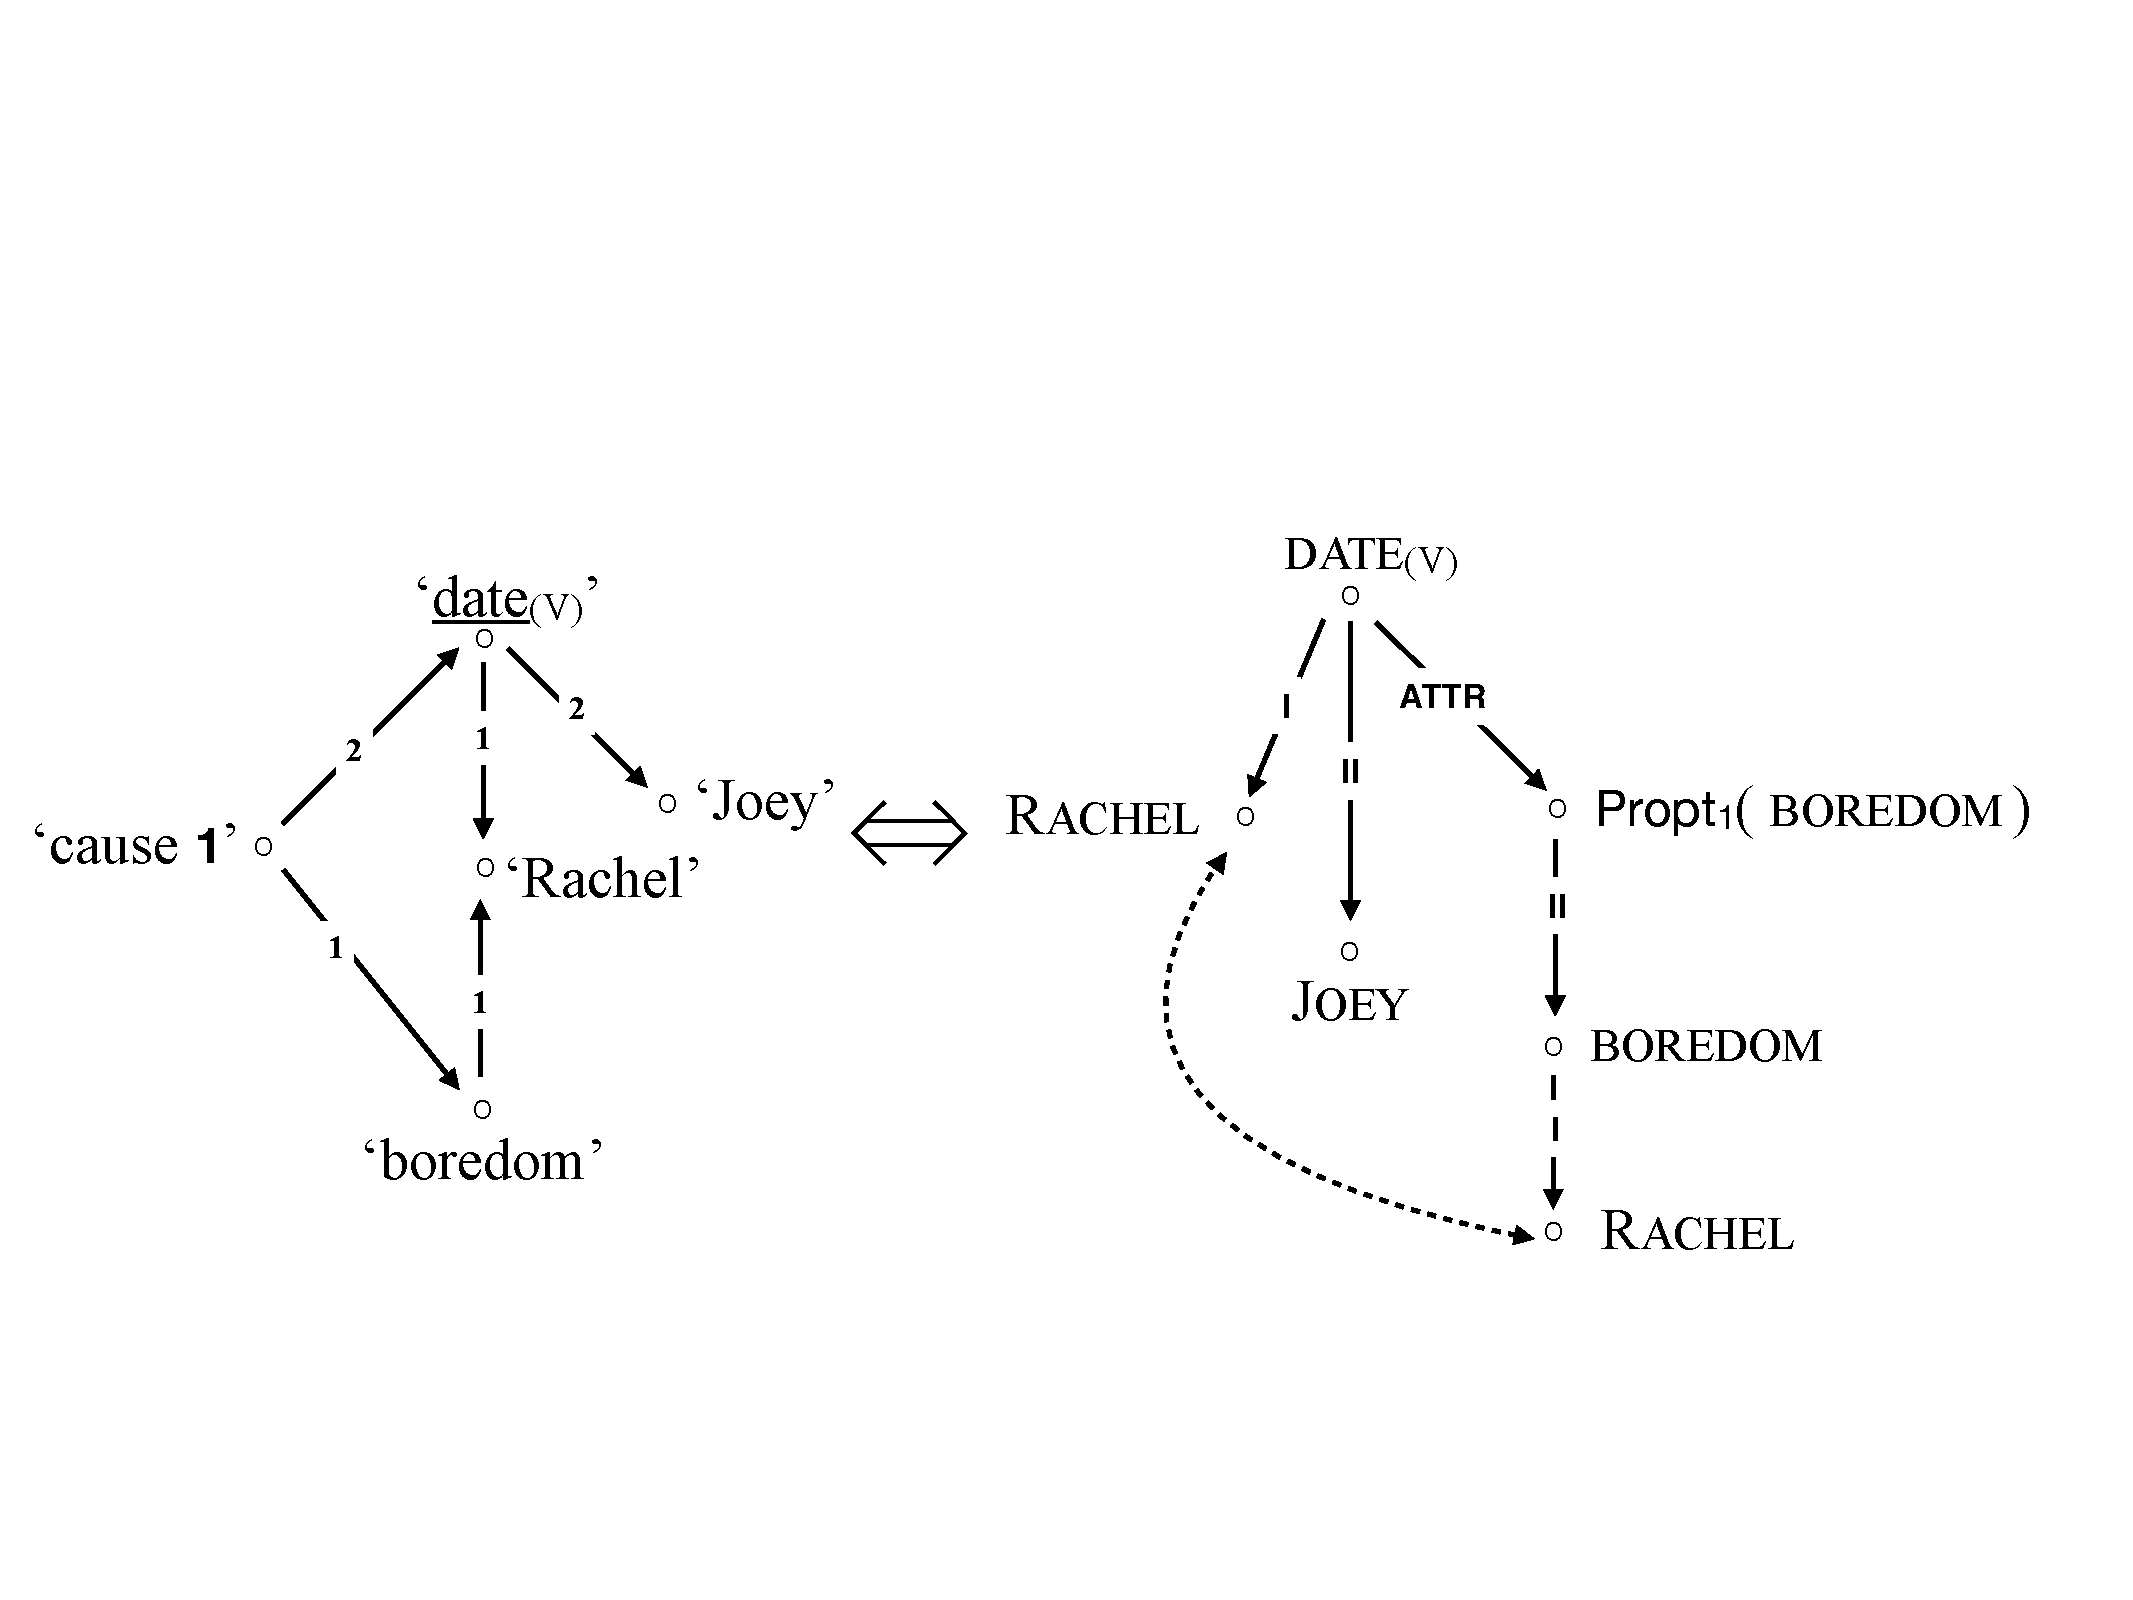
\includegraphics[width=11.5cm]{Fig/SyntLF/SemSyntPropt-i-illustr.pdf}
\caption[Illustration of \lf{Propt\tsub{1}} in the Sem\thinspace$\Leftrightarrow$\thinspace{}DSynt correspondence]{Illustration of \lf{Propt\tsub{1}} in the Sem\thinspace$\Leftrightarrow$\thinspace{}DSynt correspondence\footnotemark}\label{fig:Propt-i-illustr}
\end{figure}\footnotetext{On the non-agentive `cause\sensenum{1}' vs. the agentive `cause\sensenum{2}', see ``\nameref*{par:Cause1Cause2},'' p.\thinspace\pageref{par:Cause1Cause2}.}

Because of its meaning, \lf{Propt\tsub{i}} is naturally related to the LF \lf{Caus}\index[lf]{Caus@\lf{Caus}} (\sectref{sec:collocCausatif}, [\ref{lf:Caus}], p.\thinspace\pageref{lf:Caus}), such that it is possible to write the following deep-syntactic paraphrasing rule for \lf{Propt\tsub{1}}\index[lf]{Propti@\lf{Propt\tsub{i}}!\lf{Propt\tsub{1}}}:

\begin{center}
\phantomsection\label{txt:RParaphPropt1}\APolbox{11.6cm}{%
\textbf{R\tsub{\lf{Propt$_\text{1}$}}:} \\*
{L\tsub{(V)}\thinspace\syntRel{ATTR}\thinspace\lfappl{Propt\tsub{i}}{L}\syntRel{II}L\enskip{\small$\equiv$}\enskip{}L\thinspace\syntRelLeft{I}\thinspace\lfappl{CausFunc\tsub{0}}{\lfappl{S\tsub{0}}{L\tsub{(V)}}}\thinspace\syntRel{II}\thinspace\lfappl{S\tsub{0}}{L\tsub{(V)}}} \\*[3pt] 
\small
\begin{tabular}{p{10.8cm}}
\leftskip=0.5cm\textit{The bar closed for}\tsub{\lfappl{Propt$_\text{1}$}{\textit{lack}\tsub{(N)}}} \textit{lack of customers.} \\
\leftskip=0.5cm$\equiv$ \\
\leftskip=0.5cm\textit{The lack of customers lead}\tsub{\lfappl{CausFunc$_\text{0}$}{\lfappl{S$_\text{0}$}{\textit{close}\tsub{(V)}}}} \textit{to the closure}\tsub{\lfappl{S$_\text{0}$}{\textit{close}\tsub{(V)}}} \textit{of the bar.}
\end{tabular}
}
\end{center}\index[notion]{paraphrase!deep-syntactic paraphrasing rule!\textbf{R\tsub{\lf{Propt$_\text{1}$}}}|emph}

\begin{quote}
\begingroup
\small
\begin{tabular}{ l c }
   \midrule
   \multicolumn{2}{l}{\lf{Propt\tsub{i}}: adverbial} \\
   \midrule
   \textbf{L} & N \\
   \midrule
   \textbf{\lfappl{Propt\tsub{i}}{L}} & Adv \\
   \midrule
\end{tabular}
\endgroup
\end{quote}

\phantomsection\label{txt:Propt1UnderTheEffectOfAlcohol}\begin{longtable*}[l]{ l l >{\raggedright\arraybackslash}p{7cm} }

\multicolumn{3}{l}{\textbf{English}} \\*

\lfappl{Propt\tsub{1}}{\textit{interest}\tsub{(N)}} & = & \textit{out}\onewdf\textit{of} \lfgp{\textsc{art} \tld} \\
\lfappl{Propt\tsub{1}}{\textit{alcohol}} & = & \textit{under the effect} \lfgp{\textit{of} \tld}\textbf{;} \fused\idiom{\textit{under the influence}} \\
\lfappl{Propt\tsub{1}}{\textit{combat}\tsub{(N)}} & = & \textit{in} \lfgp{\tld} \\
\lfappl{Propt\tsub{1}}{\textit{\idiom{heart attack}}} & = & \textit{of} \lfgp{\textsc{(art)} \tld} \\
\lfappl{Propt\tsub{1}}{\textit{lack}\tsub{(N)}} & = & \textit{for} \lfgp{\tld} \\
\multicolumn{3}{l}{\quad\lfgp{N\tsub{X}\textit{'s lack of} N\tsub{Y}}} \\
\lfappl{Propt\tsub{2}}{\textit{attack}} & = & \textit{in} \lfgp{\textsc{art} \tld} \\[6pt]

\multicolumn{3}{l}{\textbf{French}} \\*

\lfappl{Propt\tsub{1}}{\textit{intérêt}} & = & \textit{par} \lfgp{\tld} \\
\lfappl{Propt\tsub{1}}{\textit{alcool}} & = & \textit{sous l'emprise} \lfgp{\textit{de} \textsc{art} \tld} \\
\lfappl{Propt\tsub{1}}{\textit{combat}} & = & \textit{à} \lfgp{\textit{le} \tld} \lfgp{$\Rightarrow$ \textit{au combat}} \\
\lfappl{Propt\tsub{1}}{\textit{\idiom{crise cardiaque}}} & = & \textit{de} \lfgp{\textsc{(art)} \tld} \\
\lfappl{Propt\tsub{2}}{\textit{manque}} & = & \textit{par} \lfgp{\tld} \\
\multicolumn{3}{l}{\quad\lfgp{\textit{manque de} N\tsub{X} \textit{pour} N\tsub{Y}}} \\
\lfappl{Propt\tsub{2}}{\textit{attentat}} & = & \textit{dans} \lfgp{\textsc{art} \tld} \\[6pt]

\multicolumn{3}{l}{\textbf{Russian}} \\*

\lfappl{Propt\tsub{1}}{\textit{interes}} & = & \textit{iz} \lfgp{\tld\textit{a}} \\
\lfappl{Propt\tsub{1}}{\textit{alkogol\suffixsplit{}\palati}} & = & \textit{pod vozdejstviem} \lfgp{\tld\textit{ja}} \\
\lfappl{Propt\tsub{1}}{\textit{boj}} & = & \textit{v}\sensenum{1} \lfgp{\tld\textit{u}} \\
\lfappl{Propt\tsub{1}}{\textit{infarkt}} & = & \textit{ot} \lfgp{\tld\textit{a}} \\
\lfappl{Propt\tsub{2}}{\textit{otsutstvi\suffixsplit{}e}} & = & \textit{iz-za} \lfgp{\tld\textit{ja}} \\
\multicolumn{3}{l}{\quad\lfgp{\textit{otsutstvie} N\tsub{X-GEN} \textit{u} N\tsub{Y-GEN}}} \\
\lfappl{Propt\tsub{2}}{\textit{pokušeni\suffixsplit{}e}} & = & \textit{v rezul\palati{}tate} \lfgp{\tld\textit{ja}} \\

\end{longtable*}

The syntagmatic LF \lf{Propt\tsub{1}}, which includes causation\index[notion]{causation}, should not be mistaken for the non-causative paradigmatic LF\index[notion]{lexical function!paradigmatic vs. syntagmatic \tlds} \lf{Adv\tsub{1}}\index[lf]{Advi@\lf{Adv\tsub{i}}};  cf. the following contrast:

\begingroup
\small

\ex. \begingroup\setlength{\tabcolsep}{2pt}
\begin{tabular}[t]{ l l >{\raggedright\arraybackslash}p{7cm} }
\lfappl{Adv\tsub{1}}{\textit{affection}} & = & \textit{affectionately}\textbf{,} \textit{with} \tld \\*
\multicolumn{3}{l}{vs.} \\*
\lfappl{Propt\tsub{1}}{\textit{affection}} & = & \textit{out}\onewdf\textit{of} \lfgp{\tld} \\
\end{tabular}\endgroup

\endgroup

See also, on \lf{Adv\tsub{i}}, \chapref{chap:paraLFs}, \sectref{sec:derivAdvAct}, [\ref{lf:Adv-i}], p.\thinspace\pageref{lf:Adv-i}. For a detailed study of \lf{Propt\tsub{i}}, see \textcite[503--617]{IordanskajaMelcuk2007}.\phantomsection\label{txt:endPropt-i}

\section{Verbal collocates}\label{sec:verbalCollocates}

\subsection{Copula verb}\label{sec:verbeCopule}\index[notion]{copula verb}\index[notion]{verb!copula \tld}

\refstepcounter{LFlist}
\subsubsection*{{\small [\arabic{LFlist}]} \lf{Copul} \lfgp{{\scriptsize Latin} \textit{copula}}: verb that means `be'}\label{lf:Copul}
\addcontentsline{toc}{subsection}{{\footnotesize [\arabic{LFlist}]} \lf{Copul}: verb that means `be'}\index[lf]{Copul@\lf{Copul}|emph}

\lfappl{Copul}{L} is a verb that means `be\tsub{(copula)}' and applies to a nominal or adjectival\slashs{}adverbial lexical unit L. It takes L as DSyntA\thinspace\syntDname{II}; its DSyntA\thinspace\syntDname{I} is the DSyntA\thinspace\syntDname{I} of L.

\begin{quote}
\begingroup
\small
\begin{tabular}{ l c c c }
   \midrule
   \multicolumn{4}{l}{\lf{Copul}: verbal} \\
   \midrule
   \textbf{L} & N & Adj & Adv \\
   \midrule
   \textbf{\lfappl{Copul}{L}} & V & V & V \\
   \midrule
\end{tabular}
\endgroup
\end{quote}

\begin{longtable*}[l]{ l l >{\raggedright\arraybackslash}p{6cm} }

\multicolumn{3}{l}{\textbf{English}} \\*

\lfappl{Copul}{\textit{example}} & = & \textit{be} \lfgp{\textsc{art} \tld}\textbf{,} \textit{serve} \lfgp{\textit{as an} \tld} \\
\lfappl{Copul}{\textit{challenge}\tsub{(N)}} & = & \textit{be}\textbf{,} \textit{constitute}\textbf{,} \textit{represent} \lfgp{\textsc{art} \tld} \\
\lfappl{Copul}{\textit{true}} & = & \textit{be}\textbf{,} \textit{hold} \lfgp{\tld} \\
\lfappl{IncepCopul}{\textit{dead}\tsub{(Adj)}} & = & \textit{drop} \lfgp{\tld} \\[6pt]

\multicolumn{3}{l}{\textbf{French}} \\*

\lfappl{Copul}{\textit{exemple}} & = & \textit{être} \lfgp{\textsc{art} \tld}\textbf{,} \textit{servir} \lfgp{\textit{d'}\tld} \\
\lfappl{Copul}{\textit{défi}} & = & \textit{être}\textbf{,} \textit{constituer}\textbf{,} \textit{représenter} \lfgp{\textsc{art} \tld} \\
\lfappl{IncepCopul}{\textit{amoureux}\tsub{(Adj)}} & = & \textit{tomber} \lfgp{\tld} \\[6pt]

\multicolumn{3}{l}{\textbf{Russian}} \\*

\lfappl{Copul}{\textit{primer}} & = & \textit{byt\palati}\textbf{,} \textit{slu\v{z}it\palati} \lfgp{\tld\textit{om}} \\
\lfappl{IncepCopul}{\textit{zamertvo}} & = & \textit{upast\palati} \lfgp{\tld} \\
\lfappl{IncepCopul}{\textit{vljublënnyj}} & = & \fused\textit{vljubit\palati{}sja} \\

\end{longtable*}

\lf{Copul} is an analytic\index[notion]{derivative!analytic semantic \tld} variant of the paradigmatic LF \lf{Pred}\index[lf]{Pred@\lf{Pred}}\index[notion]{lexical function!paradigmatic vs. syntagmatic \tlds} (\chapref{chap:paraLFs}, [\ref{lf:Pred}], p.\thinspace\pageref{lf:Pred}), so that the following equivalence holds: \lfappl{Copul}{L}\thinspace\syntRel{II}\thinspace{}L\enskip{\small$\equiv$}\enskip\lfappl{Pred}{L}. For instance:

\begingroup
\small

\ex. Her declaration was\tsub{\lfappl{Copul}{\textit{unexpected}}} unexpected.\\
     $\equiv$ \\
     Her declaration \idiom{came as a bolt from the blue}\tsub{\lfappl{Pred}{\textit{unexpected}}}.

\endgroup

\lf{Copul} does not have many values in any given natural language. It is mainly used within complex LFs, as in \lf{IncepCopul}\index[lf]{Incep@\lf{Incep}}, etc.

%\lfappl{Copul}{L} can be semantically (quasi-)equivalent to \lfappl{Oper\tsub{1}}{L} (Sec.~\ref{sec:verbeSupport} below, [\ref{lf:Oper-i}], p.\thinspace\pageref{lf:Oper-i}) if L is an Adj\slashs{}Adv or a quasi-predicative N semantically close to an Adj (\textsc{idiot}\tsub{(N)}, \textsc{genius}, etc.).

\subsection{Support [=~light] verbs}\label{sec:verbeSupport}\index[notion]{support verb|emph}\index[notion]{verb!support \tld|emph}

All LFs \lf{f} introduced in this section are ``pure'' verbalizers\index[notion]{verbalizer}. They are such that:

\begin{itemize}

\item \lf{f} applies to a non-verbal lexical unit L, and \lfappl{f}{L} takes L as DSyntA\thinspace\syntDname{I} (i.e., subject)\index[notion]{subject, syntactic} or DSyntA\thinspace\syntDname{II}\slashs\syntDname{III}\slashs... (i.e., object)\index[notion]{object, syntactic};

\item \lfappl{f}{L} is not selected by the Speaker\index[notion]{Speaker, the} to express a given meaning, but in order to construct a well-formed verbal syntactic structure with the same meaning as L.

\end{itemize}

Each \lfappl{f}{L} of this type, so to speak, ``supports'' a non-verbal L, by enabling the collocation \lfappl{f}{L}\thinspace$\rightarrow$\thinspace{}L to function as the syntactic head of the clause; hence the term \notion{support verb} \parencite{GrossM1981}. Because support verbs are semantically ``light,'' i.e. they do not semantically contribute to the sentence, they are also referred to as \notion{light verbs}\index[notion]{light verb|see{support verb}}\index[notion]{verb!light \tld|see{support verb}}, a term generally attributed to \textcite[Ch.~VII, \S\thinspace7.2{\footnotesize 1--5}]{Jespersen1946}.%\footnote{For a comparison between the notion of support verb and the closely related notion of \textit{Funktionsverb} in German studies, see \textcite{Langer2005}.}

\begin{soundboxnotitle}
A support verb is semantically empty in the collocation it forms with L in actual utterances. But this does not prevent it from having an inherent meaning in the lexicon\index[notion]{lexicon}, this meaning becoming redundant with respect  to that of L. Such is the case, for instance, of the verb \textsc{feel}\tsub{(V)} in the collocation \textit{feel pain}, the verb \textsc{face}\tsub{(V)} in \textit{face an ultimatum}, etc.
\end{soundboxnotitle}

There are three types of support verbs according to the position of the collocation base L in their DSynt-actantial structure: \lf{Oper\tsub{i}}, \lf{Func\tsub{i}} and \lf{Labor\tsub{ij}}. These three LFs have the same PoS table:

\begin{quote}
\begingroup
\phantomsection\label{tab:PdDVSup}\small
\begin{tabular}{ l c c c }
   \midrule
   \multicolumn{4}{l}{\lf{Oper\tsub{i}}, \lf{Func\tsub{i}}, \lf{Labor\tsub{ij}}: verbal} \\
   \midrule
   \textbf{L} & N & Adj & Adv \\
   \midrule
   \textbf{\lfappl{Oper\tsub{i}\slashs{}Func\tsub{i}\slashs{}Labor\tsub{ij}}{L}} &V & V & V \\
   \midrule
\end{tabular}
\endgroup
\end{quote}

A typical support verb collocation is controlled by a nominal base; almost all examples that follow present this type of collocation. However, adjectival and adverbial bases for such collocations are limitedly possible; a few illustrations are provided at the end of this section.

A support verb LF, being empty by definition, cannot be semantically characterized. We will, thus, supply for each LF described below -- \lf{Oper\tsub{i}}, \lf{Func\tsub{i}} and \lf{Labor\tsub{ij}} -- a prototypical lexical equivalent, so that the reader can have an intuitive feeling of its usage (cf. \textsc{do}\tsub{(V)} for \lf{Oper\tsub{i}}).

\refstepcounter{LFlist}
\subsubsection*{{\small [\arabic{LFlist}]} \lf{Oper\tsub{i}} \lfgp{{\scriptsize Latin} \textit{oper\={a}ri} `do, carry out'}: support verb analogous to \textsc{do}\tsub{(V)}\label{lf:Oper-i}}
\addcontentsline{toc}{subsection}{{\footnotesize [\arabic{LFlist}]} \lf{Oper\tsub{i}}: support verb analogous to \textsc{do}\tsub{(V)}}\index[lf]{Operi@\lf{Oper\tsub{i}}|emph}

\lfappl{Oper\tsub{i}}{L} is a support verb that takes L as DSyntA\thinspace\syntDname{II} and the DSyntA\thinspace\syntDname{i} of L as DSyntA\thinspace\syntDname{I}.

\lf{Oper\tsub{i}} participates in the Sem\thinspace$\Leftrightarrow$\thinspace{}DSynt\index[notion]{structure!semantic \tld\ [SemS]}\index[notion]{semantic!\tld\ structure [SemS]}\index[notion]{structure!deep-syntactic \tld\ [DSyntS]}\index[notion]{deep-syntactic!\tld\ structure [DSyntS]} correspondence\index[notion]{correspondence between representation levels} shown in \figref{fig:Oper-i}.

\begin{figure}
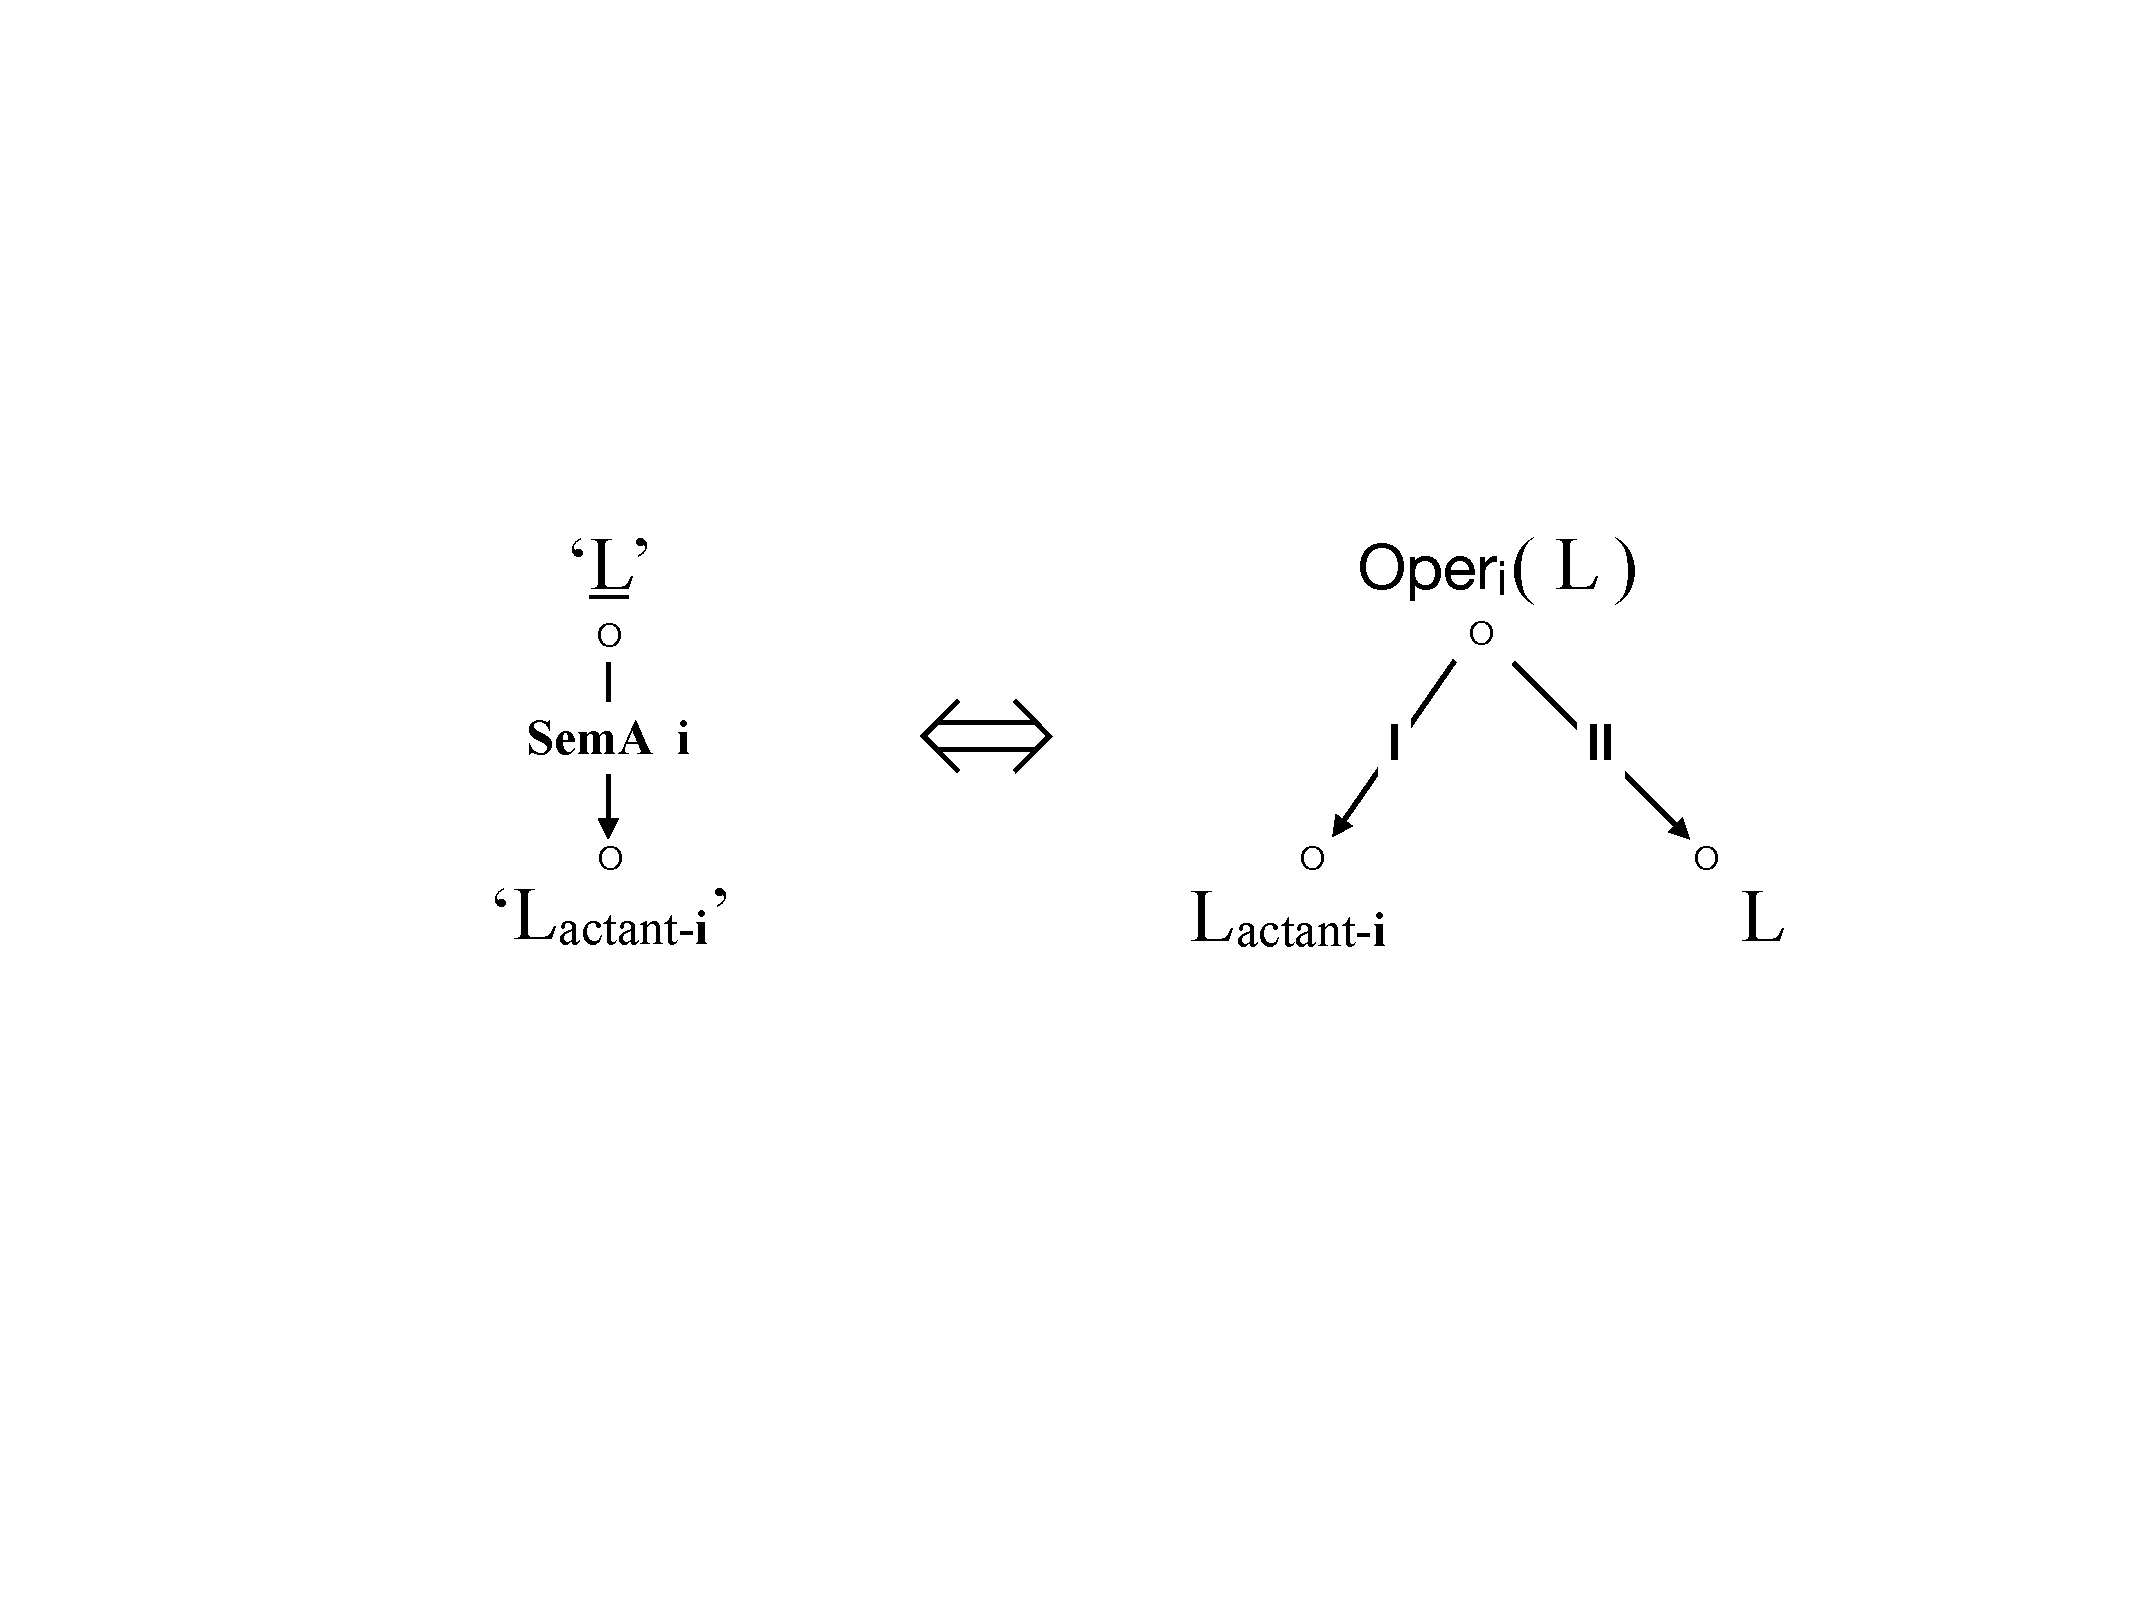
\includegraphics[height=22mm]{Fig/SyntLF/SemSyntOper-i.pdf}
\caption{\lf{Oper\tsub{i}} in the Sem\thinspace$\Leftrightarrow$\thinspace{}DSynt correspondence}\label{fig:Oper-i}
\end{figure}

\figref{fig:Oper-i-illustr} illustrates the correspondence template in \figref{fig:Oper-i} for \lf{Oper\tsub{1}}\index[lf]{Operi@\lf{Oper\tsub{i}}!\lf{Oper\tsub{1}}} with L~=~\textsc{fever}.

\begin{figure}
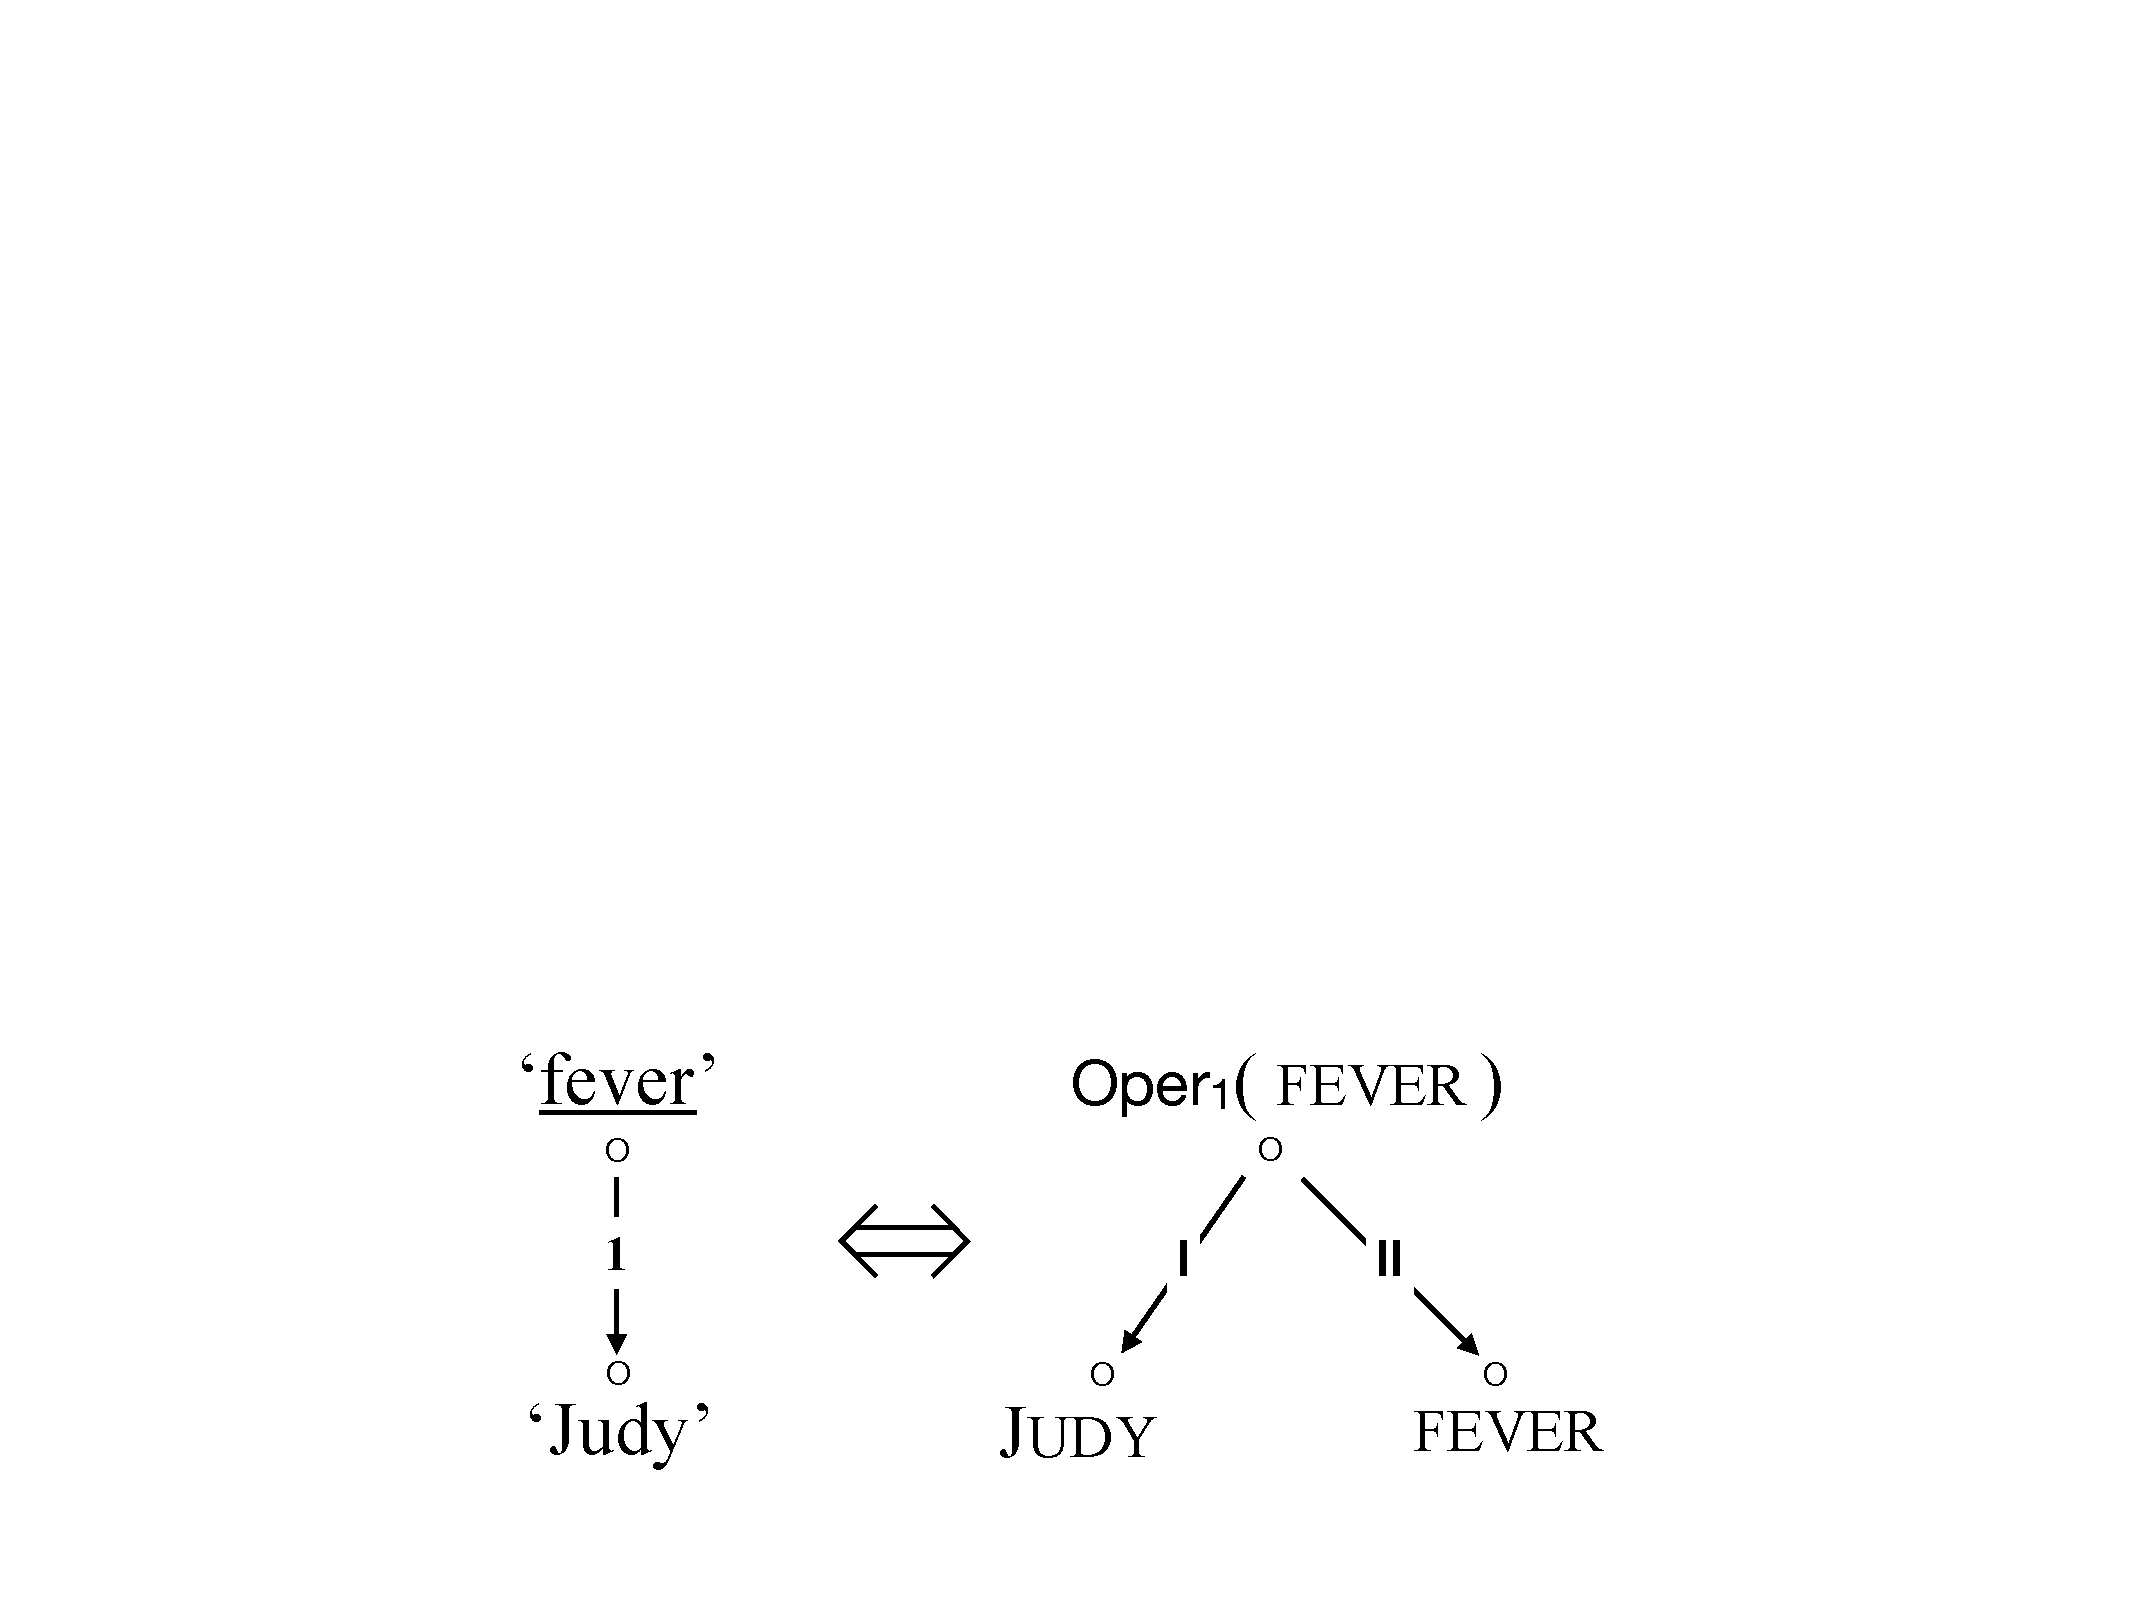
\includegraphics[height=22mm]{Fig/SyntLF/SemSyntOper-i-illustr.pdf}
\caption{\lf{Oper\tsub{1}} in the Sem\thinspace$\Leftrightarrow$\thinspace{}DSynt correspondence with L~=~\textsc{fever}}\label{fig:Oper-i-illustr}
\end{figure}

Sentences \Next[a--b] are possible implementations of the DSynt-structure given in \figref{fig:Oper-i-illustr}:

\begingroup
\small

\ex. \a. Judy \emph{has} a fever.
     \b. Judy \emph{runs} a fever.

\endgroup

\lfappl{Oper\tsub{i}}{L} can be an impersonal\index[notion]{verb!impersonal \tld}\index[notion]{impersonal verb} support verb, which has no DSyntA\thinspace\syntDname{I}. In such a case, the notation \lfappl{Oper\tsub{0}}{L}\index[lf]{Operi@\lf{Oper\tsub{i}}!\lf{Oper\tsub{0}}|emph} is used (see French and Russian illustrations below).

\begin{longtable*}[l]{ l l >{\raggedright\arraybackslash}p{6cm} }

\multicolumn{3}{l}{\textbf{English}} \\*

\lfappl{Oper\tsub{1}}{\textit{crime}} & = & \textit{commit}\textbf{,} \textit{perpetrate} \lfgp{\textsc{art} \tld} \\
\lfappl{Oper\tsub{1}}{\textit{supremacy}} & = & \textit{detain} \lfgp{\textsc{art} \tld} \\
\lfappl{Oper\tsub{2}}{\textit{bullying}} & = & \textit{undergo} \lfgp{\tld} \\
\lfappl{Oper\tsub{2}}{\textit{danger}} & = &  \textit{run} \lfgp{\textsc{art} \tld} \\
\lfappl{Oper\tsub{2}}{\textit{applause}} & = & \textit{draw}\textbf{,} \textit{get}\textbf{,} \textit{win} \lfgp{\tld\ \lfconstr{with a modifier}} \\
\lfappl{Oper\tsub{3}}{\textit{order}\tsub{(N)}} & = & \textit{get}\textbf{,} \textit{receive} \lfgp{\textsc{art} \tld} \\
\multicolumn{3}{l}{\quad\lfgp{N\tsub{X}\textit{'s order to} V\tsub{Y} \textit{to} N\tsub{Z}}} \\
\lfappl{Oper\tsub{3}}{\textit{refusal}} & = & \textit{meet} \lfgp{\textit{with} \textsc{(art)} \tld} \\
\multicolumn{3}{l}{\quad\lfgp{N\tsub{X}\textit{'s refusal to} V\tsub{Y} \textit{to} N\tsub{Z}}} \\[6pt]

\multicolumn{3}{l}{\textbf{French}} \\*

\lfappl{Oper\tsub{0}}{\textit{nuit}} & = & \lfgp{\textit{il}\tsub{(impers)}} \textit{faire} \lfgp{\tld}\\
\lfappl{Oper\tsub{0}}{\textit{soif}} & = & \uslabel{informal} \lfgp{\textit{il}\tsub{(impers)}} \textit{faire} \lfgp{\tld}\\
\lfappl{Oper\tsub{1}}{\textit{méfait}} & = & \textit{perpétrer} \lfgp{\textsc{art} \tld}\\
\lfappl{Oper\tsub{1}}{\textit{suprématie}} & = & \textit{détenir} \lfgp{\textsc{art} \tld}\\
\lfappl{Oper\tsub{2}}{\textit{calomnie}} & = & \textit{subir} \lfgp{\textsc{art} \tld}\\
\lfappl{Oper\tsub{2}}{\textit{danger}} & = & \textit{courir} \lfgp{\textsc{art} \tld}\\
\lfappl{Oper\tsub{2}}{\textit{applaudissements}} & = & \textit{recueillir} \lfgp{\textsc{art} \tld}\\
\lfappl{Oper\tsub{3}}{\textit{consensus}} & = & \textit{faire} \lfgp{\tld}\\
\multicolumn{3}{l}{\quad\lfgp{\textit{concensus entre} N\tsub{X} \textit{et} N\tsub{Y} \textit{à propos de} N\tsub{Z}}} \\
\lfappl{Oper\tsub{3}}{\textit{refus}} & = & \textit{essuyer} \lfgp{\textsc{art} \tld}\textbf{,} \textit{se heurter} \lfgp{\textit{à} \textsc{art} \tld} \\*
\multicolumn{3}{l}{\quad\lfgp{\textit{refus de} N\tsub{X} \textit{de} V\tsub{Y-\textsc{inf}} \textit{à} N\tsub{Z}}} \\[6pt]

\multicolumn{3}{l}{\textbf{Russian}} \\*

\lfappl{Oper\tsub{0}}{\textit{zapax}} & = &  \textit{tjanut\palati} \lfgp{\tld\textit{om}} \\
\lfappl{Oper\tsub{0}}{\textit{proxlad\suffixsplit{}a}} & = &  \textit{vejat\palati} \lfgp{\tld\textit{oj}}  \\
\lfappl{Oper\tsub{1}}{\textit{prestupleni\suffixsplit{}e}} & = & \textit{sover\v{s}it\palati} \lfgp{\tld\textit{e}} \\
\lfappl{Oper\tsub{1}}{\textit{prevosxodstv\suffixsplit{}o}} & = & \textit{imet\palati} \lfgp{\tld\textit{o}} \\
\lfappl{Oper\tsub{2}}{\textit{izdevatel\palati{}stv\suffixsplit{}a}} & = & \textit{podvergat\palati{}sja} \lfgp{\tld\textit{am}} \\
\lfappl{Oper\tsub{2}}{\textit{opasnost\suffixsplit{}\palati}} & = &  \textit{podvergat\palati{}sja} \lfgp{\tld\textit{i}} \\
\lfappl{Oper\tsub{2}}{\textit{aplodisment\suffixsplit{}y}} & = & \textit{byt\palati\ vstre\v{c}en} \lfgp{\tld\textit{ami}} \\
\lfappl{Oper\tsub{3}}{\textit{prikaz}} & = & \textit{polu\v{c}it\palati} \lfgp{\tld} \\
\multicolumn{3}{l}{\quad\lfgp{\textit{prikaz} N\tsub{X-\textsc{gen}} N\tsub{Z-\textsc{dat}} V\tsub{Y-\textsc{inf}}}} \\
\lfappl{Oper\tsub{3}}{\textit{otkaz}} & = & \textit{natolknut\palati{}sja} \lfgp{\textit{na}\sensenum{2} \tld}\textbf{,} \textit{polu\v{c}it\palati} \lfgp{\tld} \\*
\multicolumn{3}{l}{\quad\lfgp{\textit{otkaz} N\tsub{X-\textsc{gen}} N\tsub{Z-\textsc{dat}} V\tsub{Y-\textsc{inf}}}} \\

\end{longtable*}

\lf{Oper\tsub{i}} is the most frequent among support verbs. This is explained by the following fact: the base of an \lf{Oper\tsub{i}} collocation is in most cases the direct object\index[notion]{object, syntactic!direct \tld} of the verb, and semantic constraints are the strongest between a transitive verb\index[notion]{verb!transitive \tld} and its direct object -- stronger than between a verb and its other actants. It is for this reason that natural languages phraseologize in the first place phrases of the form V\thinspace\syntRel{DirO}\thinspace{}N.

Understandably, \lf{Oper\tsub{i}} has the pride of place in paraphrasing\index[notion]{paraphrase} systems of natural languages, as illustrated by the following two cases.

\begin{enumerate}

\item \lfappl{Oper\tsub{1}}{\lfappl{S\tsub{0}}{L\tsub{(V)}}}\thinspace\syntRel{II}\thinspace\lfappl{S\tsub{0}}{L\tsub{(V)}} is a paraphrase of L\tsub{(V)}:
            
\begingroup
\small

\ex. Joey joked.\\*
     $\equiv$ \\*
     Joey cracked a joke.

\endgroup

On such equivalence, see syntactic paraphrasing rule \textbf{R\tsub{\lf{Oper$_\text{1}$}}}\index[notion]{paraphrase!deep-syntactic paraphrasing rule!\textbf{R\tsub{\lf{Oper$_\text{1}$}}}}, introduced in \chapref{chap:NotionLF}, \sectref{sec:LFStandardParaphrasing} (p.\thinspace\pageref{txt:RParaphOper1}).

\item \lf{Oper\tsub{2}} is in the same paraphrastic relation -- i.e., syntactic conversion\index[notion]{conversive} -- with \lf{Oper\tsub{1}} as found between the passive and the active voice\index[notion]{voice, grammatical} of a verb, cf. \Next[a--b]:

\begingroup
\small

\ex. \a. Rachel gave\tsub{\lf{Oper\tsub{1}}} a kiss to Joey.\\*
         $\equiv$ \\*
         Rachel kissed\tsub{active voice} Joey.\vspace{2pt}
     \b. Joey got\tsub{\lf{Oper\tsub{2}}} a kiss from Rachel.\\*
         $\equiv$ \\*
         Joey was kissed\tsub{passive voice} by Rachel.

\endgroup

\end{enumerate}

\paragraph*{Transfer of L's actants to support verbs.}\label{par:transferOfLsActants}

In collocations \lfappl{Oper\tsub{i}}{L}\thinspace\syntRel{II}\thinspace{}L\index[notion]{object, syntactic!direct \tld}, the DSyntAs of L can migrate -- i.e., be transferred under paraphrasing -- to \lfappl{Oper\tsub{i}}{L}. In other words, \lfappl{Oper\tsub{i}}{L} can host, besides its own two obligatory DSyntAs, additional \mbox{DSyntAs} coming from L. This transfer of actants\index[notion]{actant!transfer of deep-syntactic \tld} is known as (\notion{syntactic}) \notion{raising}\index[notion]{raising, syntactic} -- see \chapref{chap:preliminaryNotions}, \sectref{sec:syntacticNotions}, p.\thinspace\pageref{def:DSyntA}. It is illustrated in \ref{ex:Oper1-CRIME} with \lfappl{Oper\tsub{1}}{\textit{crime}}.\footnote{The two utterances in \ref{ex:Oper1-CRIME} are semantically quasi-equivalent: they express the same propositional meaning, but have different communicative organizations.}\index[notion]{communicative!\tld\ structure}\index[notion]{structure!communicative \tld}

\begingroup
\small

\ex.\label{ex:Oper1-CRIME} Joey committed\tsub{\lf{Oper\tsub{1}}} a terrible crime\thinspace\syntRel{II}\thinspace{}\emph{against decency}.\\*
     $\cong$ \\*
     a terrible crime that Joey committed\thinspace\syntRel{III}\thinspace{}\emph{against decency}

\endgroup

The transfer of actants from the collocation base to the verbal collocate may be performed for all types of support verbs LFs -- \lf{Oper\tsub{i}}, \lf{Func\tsub{i}} and \lf{Labor\tsub{ij}}, as well as for corresponding complex LFs (for instance, \lf{CausFunc\tsub{0}}).

\begin{furtherreading}
On support\slashs light verbs\index[notion]{support verb}\index[notion]{verb!support \tld}, see \textcite{GrossM1981}, \textcite{Melcuk2022b} and \textcite{FleischhauerRiccio2025}; on transfer of actants from a collocation base to the collocative verb, see \textcites[253--272]{AlonsoRamos2004}{AlonsoRamos2007}.
\end{furtherreading}

\refstepcounter{LFlist}
\subsubsection*{{\small [\arabic{LFlist}]} \lf{Func\tsub{i}} \lfgp{{\scriptsize Latin} *\textit{function\={a}re} `[to] function'}: support verb analogous to\newline \idiom{\textsc{take place}}}\label{lf:Func-i}
\addcontentsline{toc}{subsection}{{\footnotesize [\arabic{LFlist}]} \lf{Func\tsub{i}}: support verb analogous to \idiom{\textsc{take place}}}\index[lf]{Funci@\lf{Func\tsub{i}}|emph}

\lfappl{Func\tsub{i}}{L} is a support verb that takes L as DSyntA\thinspace\syntDname{I} and the DSyntA\thinspace\syntDname{i} of L as DSyntA\thinspace\syntDname{II}. However, it can also have only one actantial dependent\index[notion]{dependent, syntactic}: L as DSynt\thinspace\syntDname{I}. In such a case -- an absolutely intransitive construction -- the LF is denoted as \lf{Func\tsub{0}}\index[lf]{Funci@\lf{Func\tsub{i}}!\lf{Func\tsub{0}}|emph}.

\lf{Func\tsub{i}} participates in the Sem\thinspace$\Leftrightarrow$\thinspace{}DSynt\index[notion]{structure!semantic \tld\ [SemS]}\index[notion]{semantic!\tld\ structure [SemS]}\index[notion]{structure!deep-syntactic \tld\ [DSyntS]}\index[notion]{deep-syntactic!\tld\ structure [DSyntS]} correspondence\index[notion]{correspondence between representation levels} shown in \figref{fig:Func-i}; it is to be compared to the \lfappl{Oper\tsub{i}}{L}\index[lf]{Operi@\lf{Oper\tsub{i}}} correspondence in \figref{fig:Oper-i} (p.\thinspace\pageref{fig:Oper-i}).

\begin{figure}
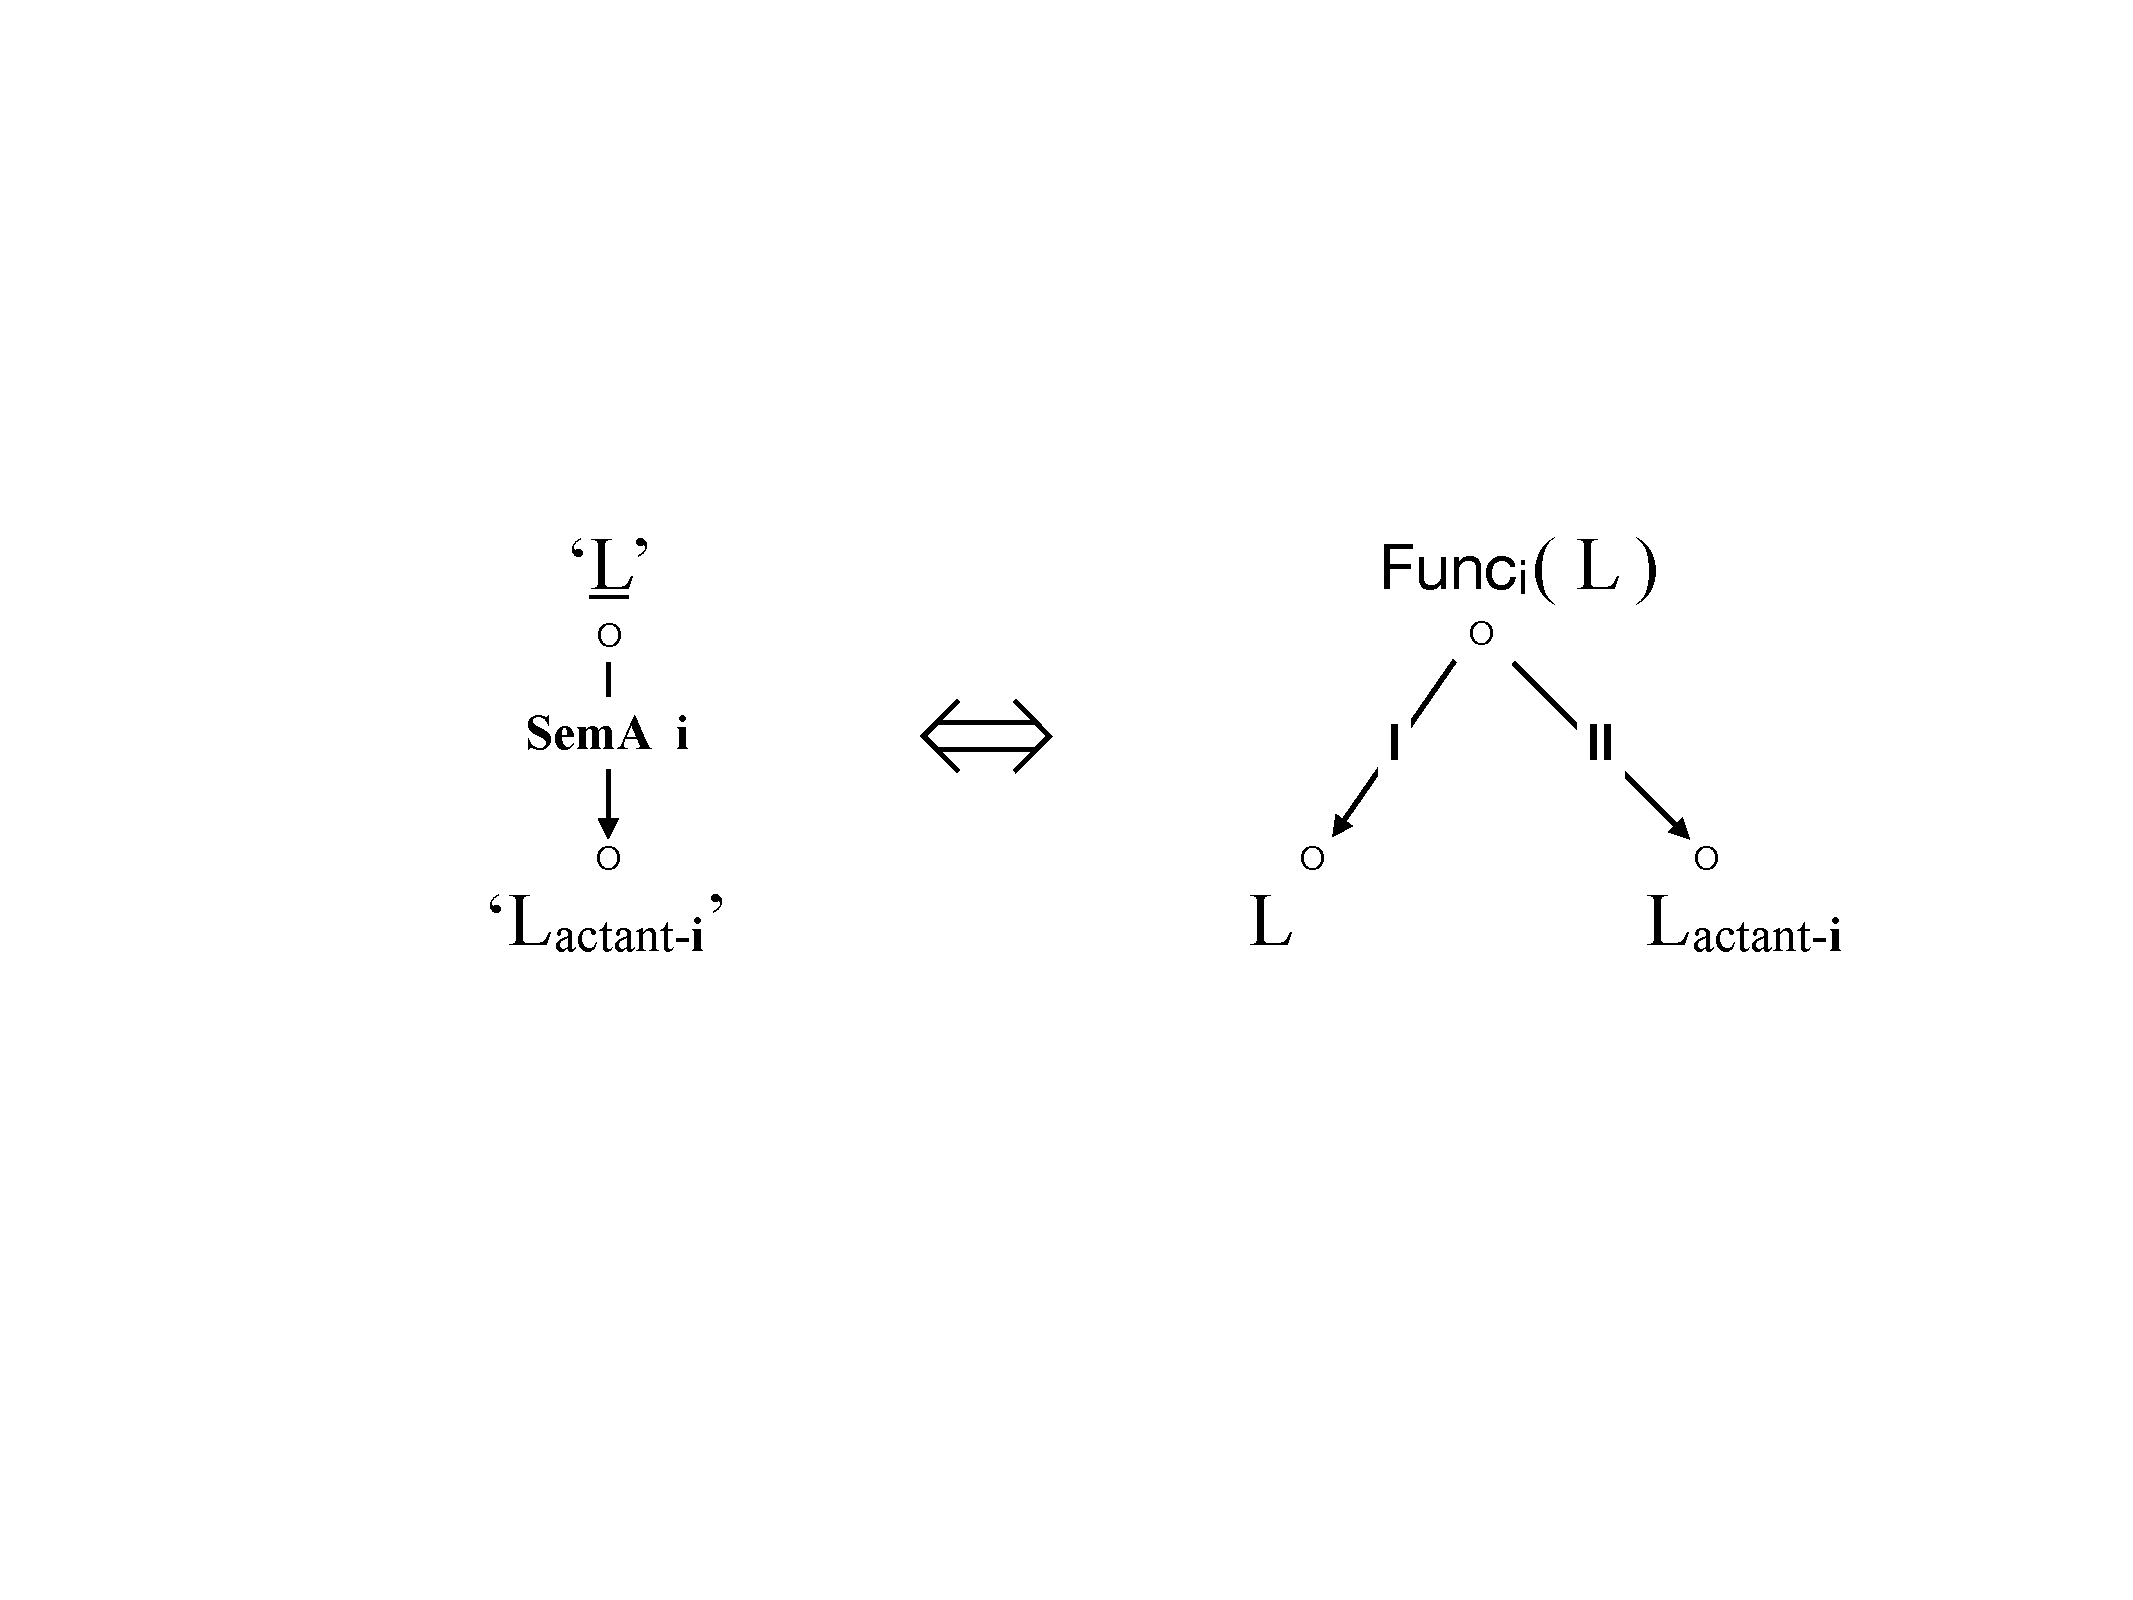
\includegraphics[height=22mm]{Fig/SyntLF/SemSyntFunc-i.pdf}
\caption{\lf{Func\tsub{i}} in the Sem\thinspace$\Leftrightarrow$\thinspace{}DSynt correspondence}\label{fig:Func-i}
\end{figure}

\figref{fig:Func-i-illustr} illustrates the correspondence template in \figref{fig:Func-i} for \lf{Func\tsub{1}} with L~= \textsc{responsibility}.

\begin{figure}
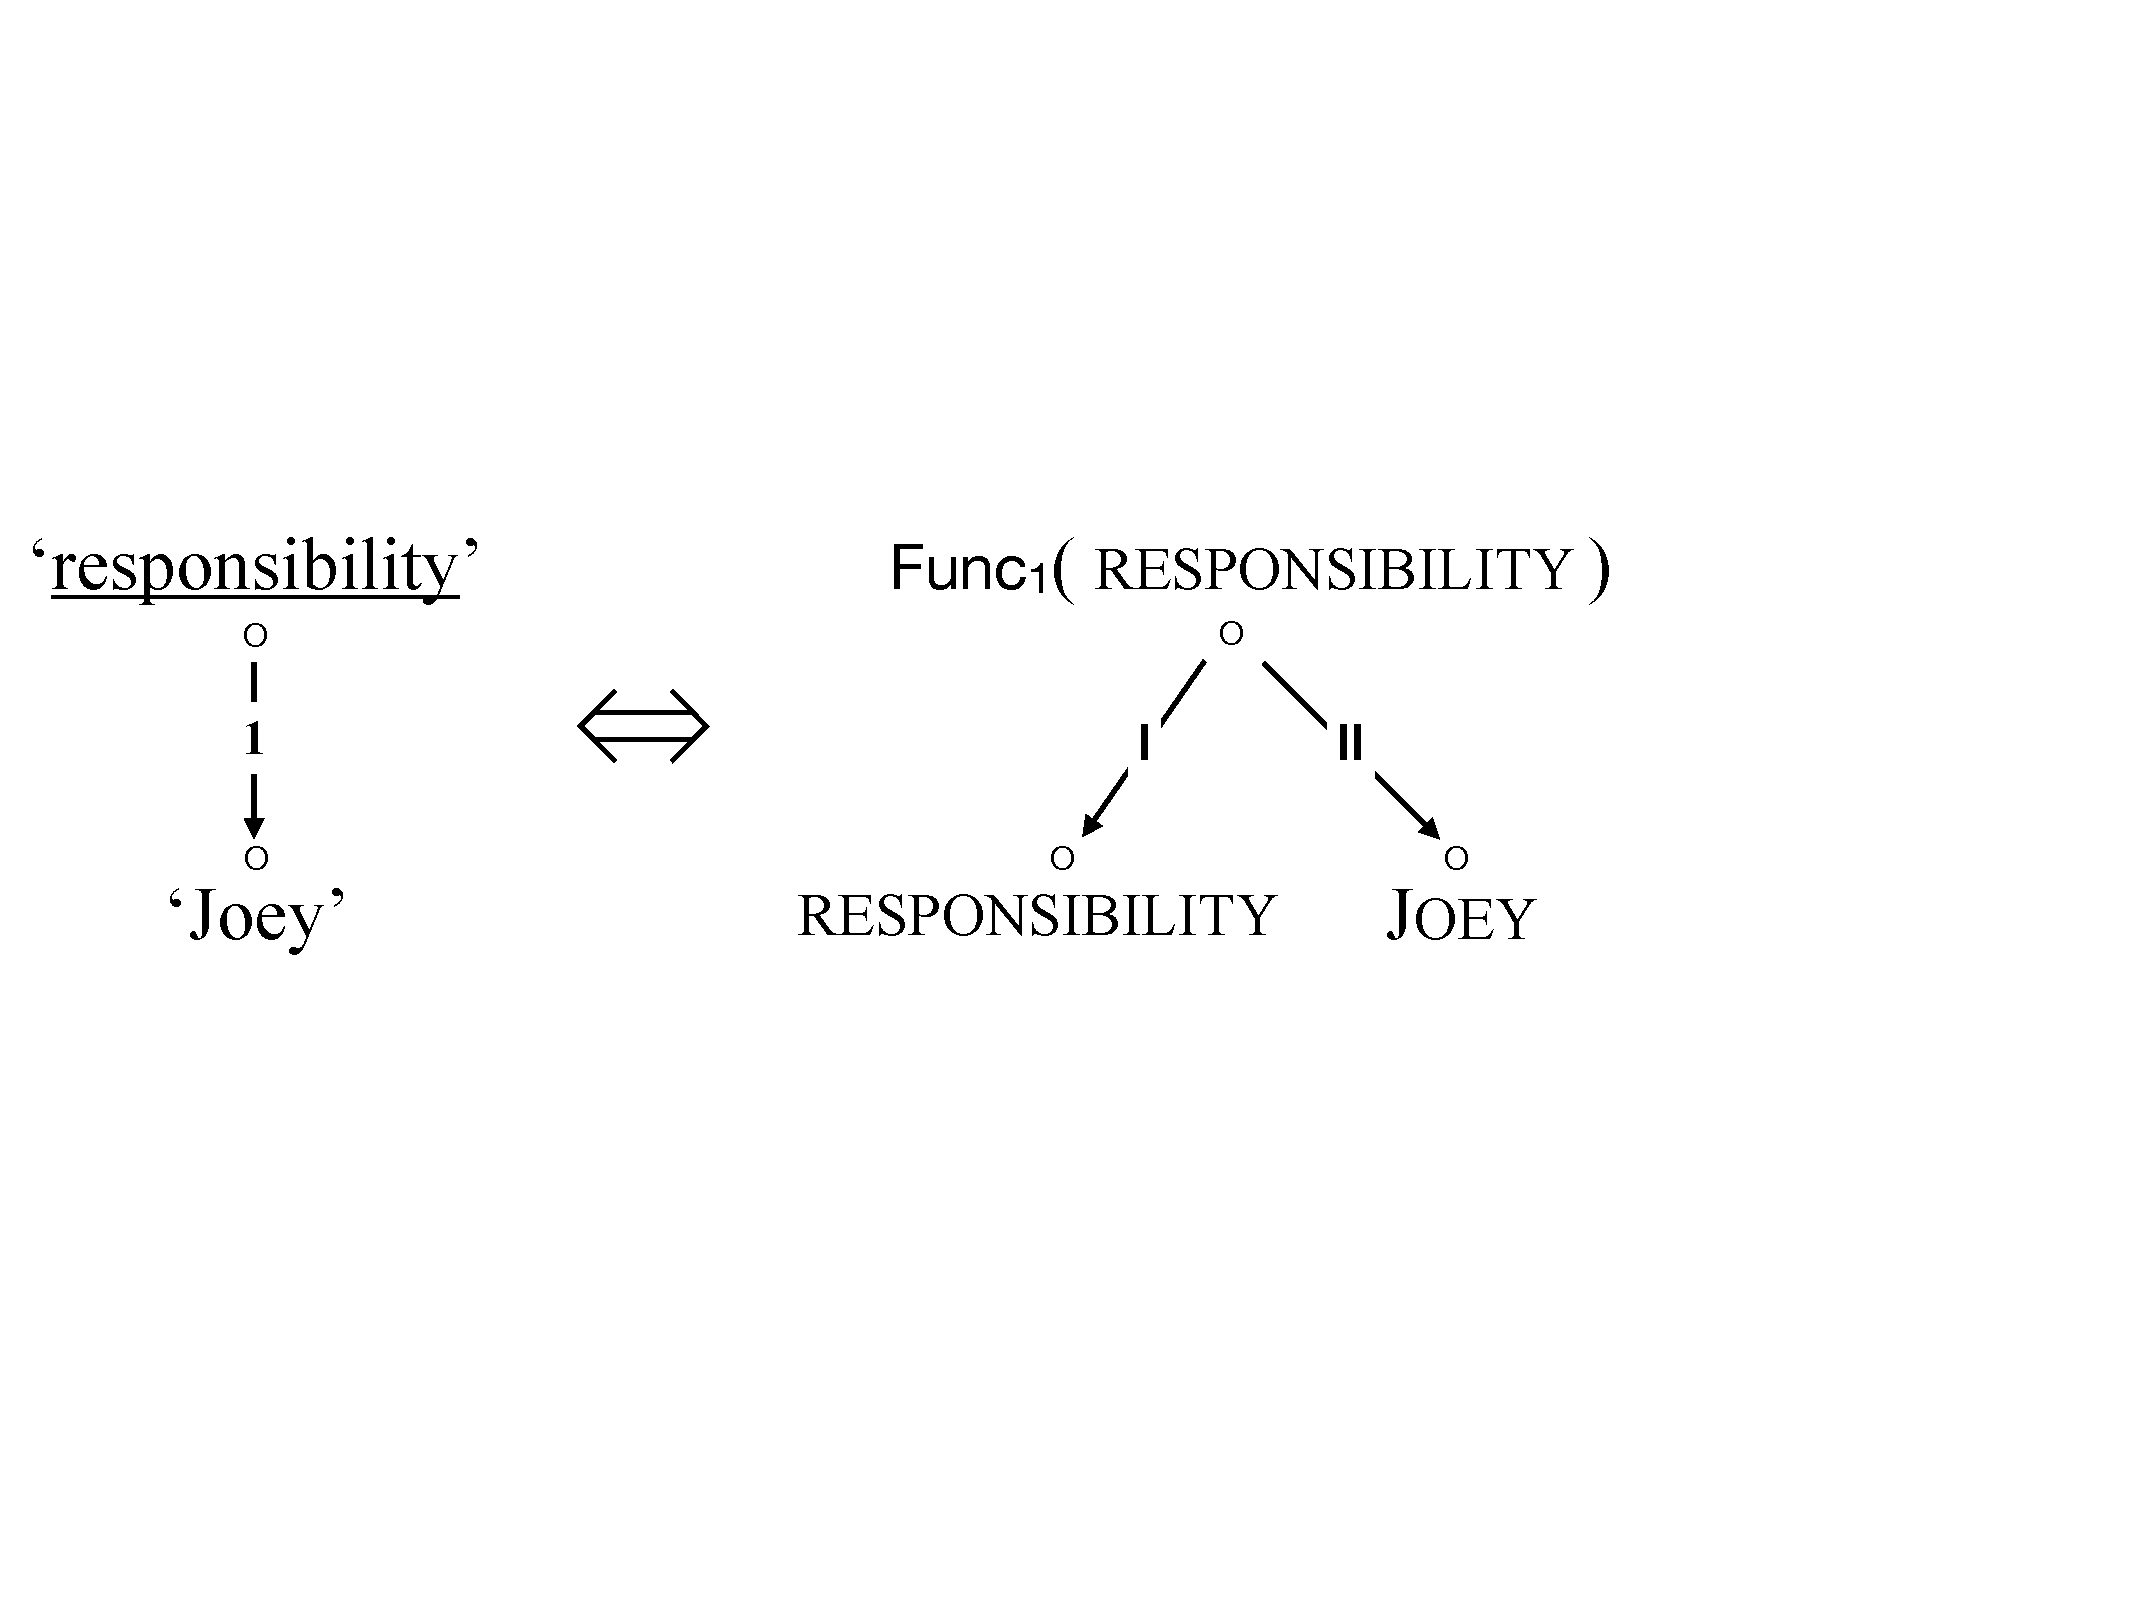
\includegraphics[height=22mm]{Fig/SyntLF/SemSyntFunc-i-illustr.pdf}
\caption{\lf{Func\tsub{1}} in the Sem\thinspace$\Leftrightarrow$\thinspace{}DSynt correspondence with L~=~\textsc{responsibility}}\label{fig:Func-i-illustr}
\end{figure}

Sentences \Next[a--b] are possible implementations of the DSynt-structure given in \figref{fig:Func-i-illustr}:

\begingroup
\small

\ex. \a. The responsibility \emph{lies} with Joey.
     \b. The responsibility \emph{rests} with Joey.

\endgroup

\begin{longtable*}[l]{ l l >{\raggedright\arraybackslash}p{6cm} }

\multicolumn{3}{l}{\textbf{English}} \\*

\lfappl{Func\tsub{0}}{\textit{thunder}\tsub{(N)}} & = & \textit{clap}\tsub{(V)}\textbf{,} \textit{crash}\tsub{(V)}\textbf{,} \textit{roll}\tsub{(V)}\textbf{,} \textit{rumble}\tsub{(V)} \\
\lfappl{Magn+Func\tsub{0}}{\textit{fire}\tsub{(N)} \lfgp{disaster}} & = & \textit{rage}\tsub{(V)} \\
\lfappl{Magn+Func\tsub{1}}{\textit{fire}\tsub{(N)} \lfgp{disaster}} & = & \textit{rip}\tsub{(V)}\textbf{,} \textit{sweep}\tsub{(V)} \lfgp{\textit{through} N\tsub{X}} \\
\lfappl{Func\tsub{1}}{\textit{responsibility} \lfgp{\textit{of} N\tsub{X}}} & = & \textit{lie}\tsub{(V)}\textbf{,} \textit{rest}\tsub{(V)} \lfgp{\textit{with} N\tsub{X}} \\
\lfappl{Func\tsub{1}}{\textit{smell}\tsub{(N)} \lfgp{\textit{of} N\tsub{X}}} & = & \textit{come}\tsub{(V)} \lfgp{\textit{from} N\tsub{X}} \\
\lfappl{Func\tsub{2}}{\textit{danger} \lfgp{\textit{for} N\tsub{Y}}} & = & \textit{threaten} \lfgp{N\tsub{Y}} \\
\lfappl{Func\tsub{2}}{\textit{accusation} \lfgp{\textit{against} N\tsub{Y}}} & = & \textit{hang}\tsub{(V)} \lfgp{\textit{over} N\tsub{Y}} \\
\lfappl{Func\tsub{3}}{\textit{conversation}} & = & \textit{be} \lfgp{\textit{about} N\tsub{Z}} \\*
\multicolumn{3}{l}{\quad\lfgp{\textit{conversation between {\upshape N\tsub{X}} and {\upshape N\tsub{Y}} about {\upshape N\tsub{Z}}}}} \\[6pt]

\multicolumn{3}{l}{\textbf{French}} \\*

\lfappl{Func\tsub{0}}{\textit{tonnerre}} & = & \textit{gronder}\textbf{,} \textit{retentir}\\
\lfappl{Magn+Func\tsub{0}}{\textit{incendie}} & = & \idiom{\textit{faire rage}}\\
\lfappl{Func\tsub{1}}{\textit{responsabilité} \lfgp{\textit{de} N\tsub{X}}} & = & \textit{incomber} \lfgp{\textit{à} N\tsub{X}}\\
\lfappl{Func\tsub{1}}{\textit{odeur} \lfgp{\textit{de} N\tsub{X}}} & = & \textit{se dégager}\textbf{,} \textit{émaner} \lfgp{\textit{de} N\tsub{X}}\\
\lfappl{Func\tsub{2}}{\textit{danger} \lfgp{\textit{pour} N\tsub{Y}}} & = & \textit{menacer} \lfgp{N\tsub{Y}}\\
\lfappl{Func\tsub{2}}{\textit{accusation} \lfgp{\textit{contre} N\tsub{Y}}} & = & \textit{frapper} \lfgp{N\tsub{Y}} \\
\lfappl{Func\tsub{3}}{\textit{conversation}} & = & \textit{porter} \lfgp{\textit{sur} N\tsub{Z}} \\*
\multicolumn{3}{l}{\quad\lfgp{\textit{conversation entre} N\tsub{X} \textit{et} N\tsub{Y} \textit{sur} N\tsub{Z}}} \\[6pt]

\multicolumn{3}{l}{\textbf{Russian}} \\*

\lfappl{Func\tsub{0}}{\textit{grom}} & = & \textit{gremet\palati}\textbf{,} \textit{gromyxat\palati} \\
\lfappl{Magn+Func\tsub{0}}{\textit{po\v{z}ar}} & = & \textit{bu\v{s}evat\palati} \\
\lfappl{Func\tsub{1}}{\textit{otvetstvennost\palati} \lfgp{N\tsub{X-\textsc{gen}}}} & = & \textit{le\v{z}at\palati} \lfgp{\textit{na}\sensenum{1} N\tsub{X-\textsc{prepos}}} \\
\lfappl{Func\tsub{1}}{\textit{zapax} \lfgp{N\tsub{X-\textsc{gen}}}} & = & \textit{idti}\textbf{,} \textit{isxodit\palati} \lfgp{\textit{ot} N\tsub{X-\textsc{gen}}} \\
\lfappl{Func\tsub{2}}{\textit{opasnost\palati} \lfgp{\textit{dlja} N\tsub{Y-\textsc{gen}}}} & = & \textit{grozit\palati}\textbf{,} \textit{ugro\v{z}at\palati} \lfgp{N\tsub{Y-\textsc{dat}}} \\
\lfappl{Func\tsub{2}}{\textit{obvinenie} \lfgp{\textit{protiv} N\tsub{Y-\textsc{gen}}}} & = & \textit{navisat\palati} \lfgp{\textit{nad} N\tsub{Y-\textsc{instr}}} \\
\lfappl{Func\tsub{3}}{\textit{razgovor}} & = & \textit{idti} \lfgp{\textit{o} N\tsub{Z-\textsc{prepos}}}\textbf{,} \textit{vertet\palati{}sja} \lfgp{\textit{vokrug} N\tsub{Z-\textsc{gen}}} \\
\multicolumn{3}{l}{\quad\lfgp{\textit{razgovor me\v{z}du} N\tsub{X-\textsc{instr}} \textit{i} N\tsub{Y-\textsc{instr}} \textit{o} N\tsub{Z-\textsc{prepos}}}} \\

\end{longtable*}

\refstepcounter{LFlist}
\subsubsection*{{\small [\arabic{LFlist}]} \lf{Labor\tsub{ij}} \lfgp{{\scriptsize Latin} \textit{labor\={a}re} `[to] work'}: support verb analogous to \textsc{submit} \lfgp{N\tsub{1}~\textit{to}~N\tsub{2}}}\label{lf:Labor-ij}
\addcontentsline{toc}{subsection}{{\footnotesize [\arabic{LFlist}]} \lf{Labor\tsub{ij}}: support verb analogous to \textsc{submit} \lfgp{N\tsub{1} \textit{to} N\tsub{2}}}\index[lf]{Laborij@\lf{Labor\tsub{ij}}|emph}

\lfappl{Labor\tsub{ij}}{L} is a support verb that takes L as its most oblique [=~most peripheral] DSyntA. Its DSyntA\thinspace\syntDname{I} corresponds to L's DSyntA\thinspace\syntDname{i} and its DSyntA\thinspace\syntDname{II} corresponds to L's DSyntA\thinspace\syntDname{j}.

\lf{Labor\tsub{ij}} participates in the Sem\thinspace$\Leftrightarrow$\thinspace{}DSynt\index[notion]{structure!semantic \tld\ [SemS]}\index[notion]{semantic!\tld\ structure [SemS]}\index[notion]{structure!deep-syntactic \tld\ [DSyntS]}\index[notion]{deep-syntactic!\tld\ structure [DSyntS]} correspondence\index[notion]{correspondence between representation levels} shown in \figref{fig:Labor-ij}; \figref{fig:Labor-ij-illustr} illustrates the correspondence template in \figref{fig:Labor-ij} for \lf{Labor\tsub{12}} with L~= \mbox{\textsc{applause}}.

\begin{figure}
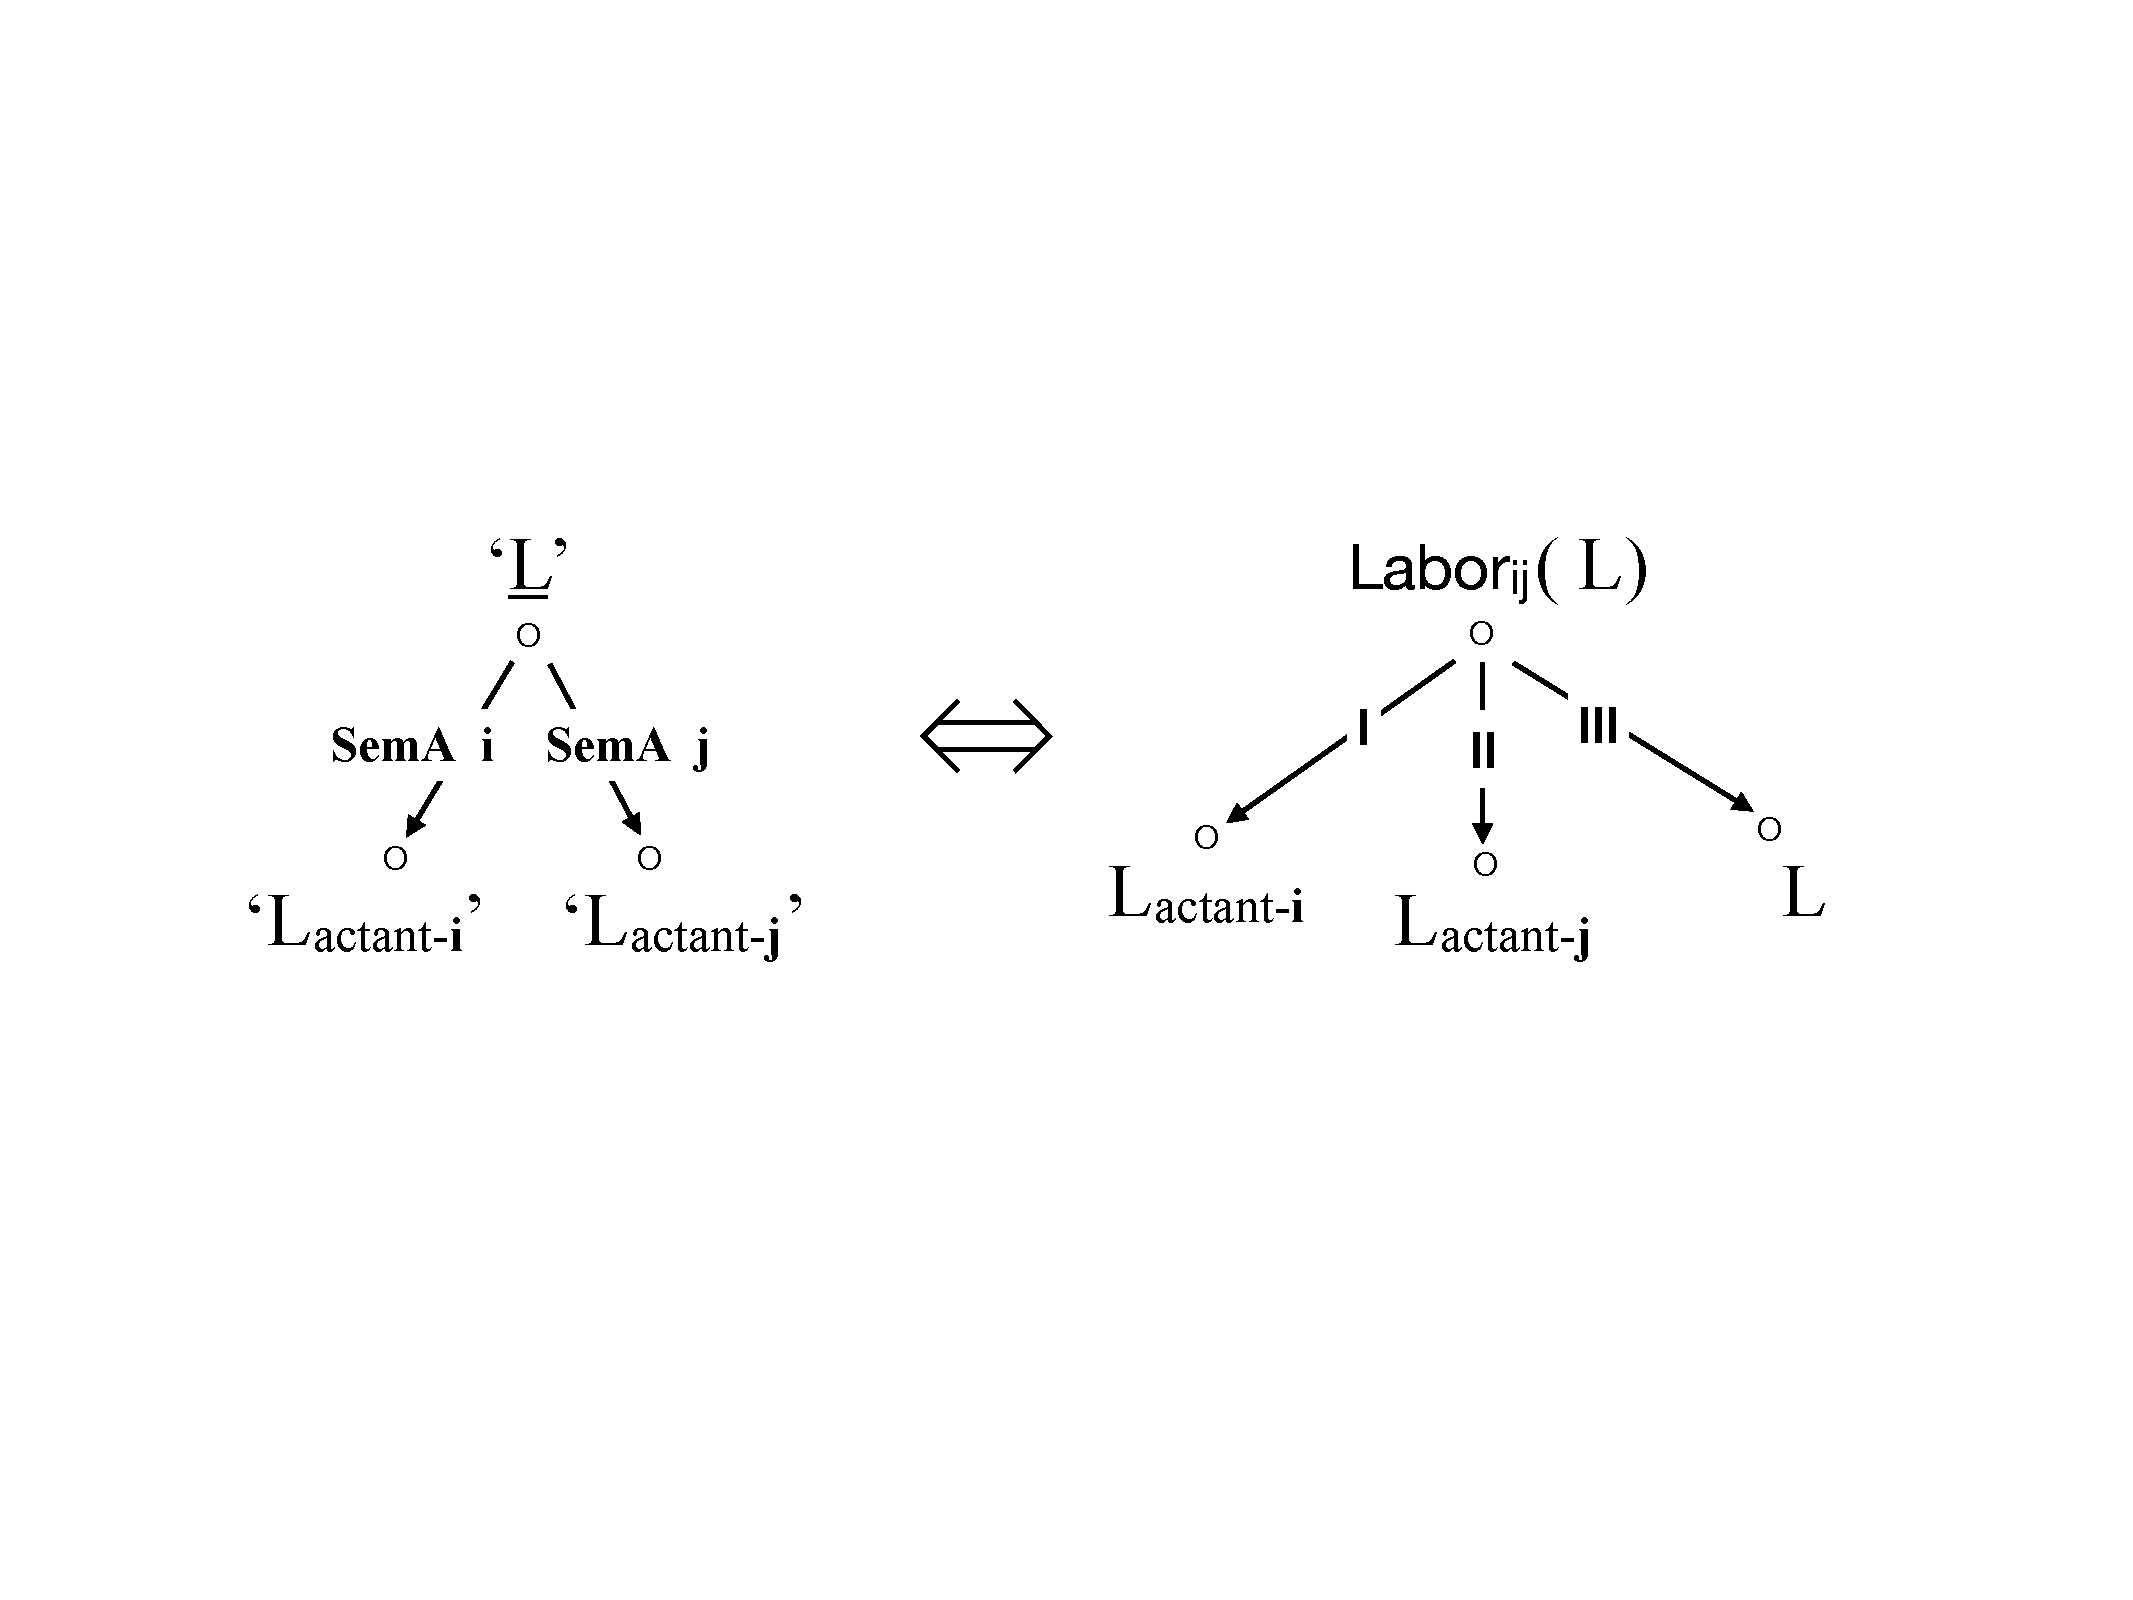
\includegraphics[width=0.65\linewidth]{Fig/SyntLF/SemSyntLabor-ij.pdf}
\caption{\lf{Labor\tsub{ij}} in the Sem\thinspace$\Leftrightarrow$\thinspace{}DSynt correspondence}\label{fig:Labor-ij}
\end{figure}

\begin{figure}
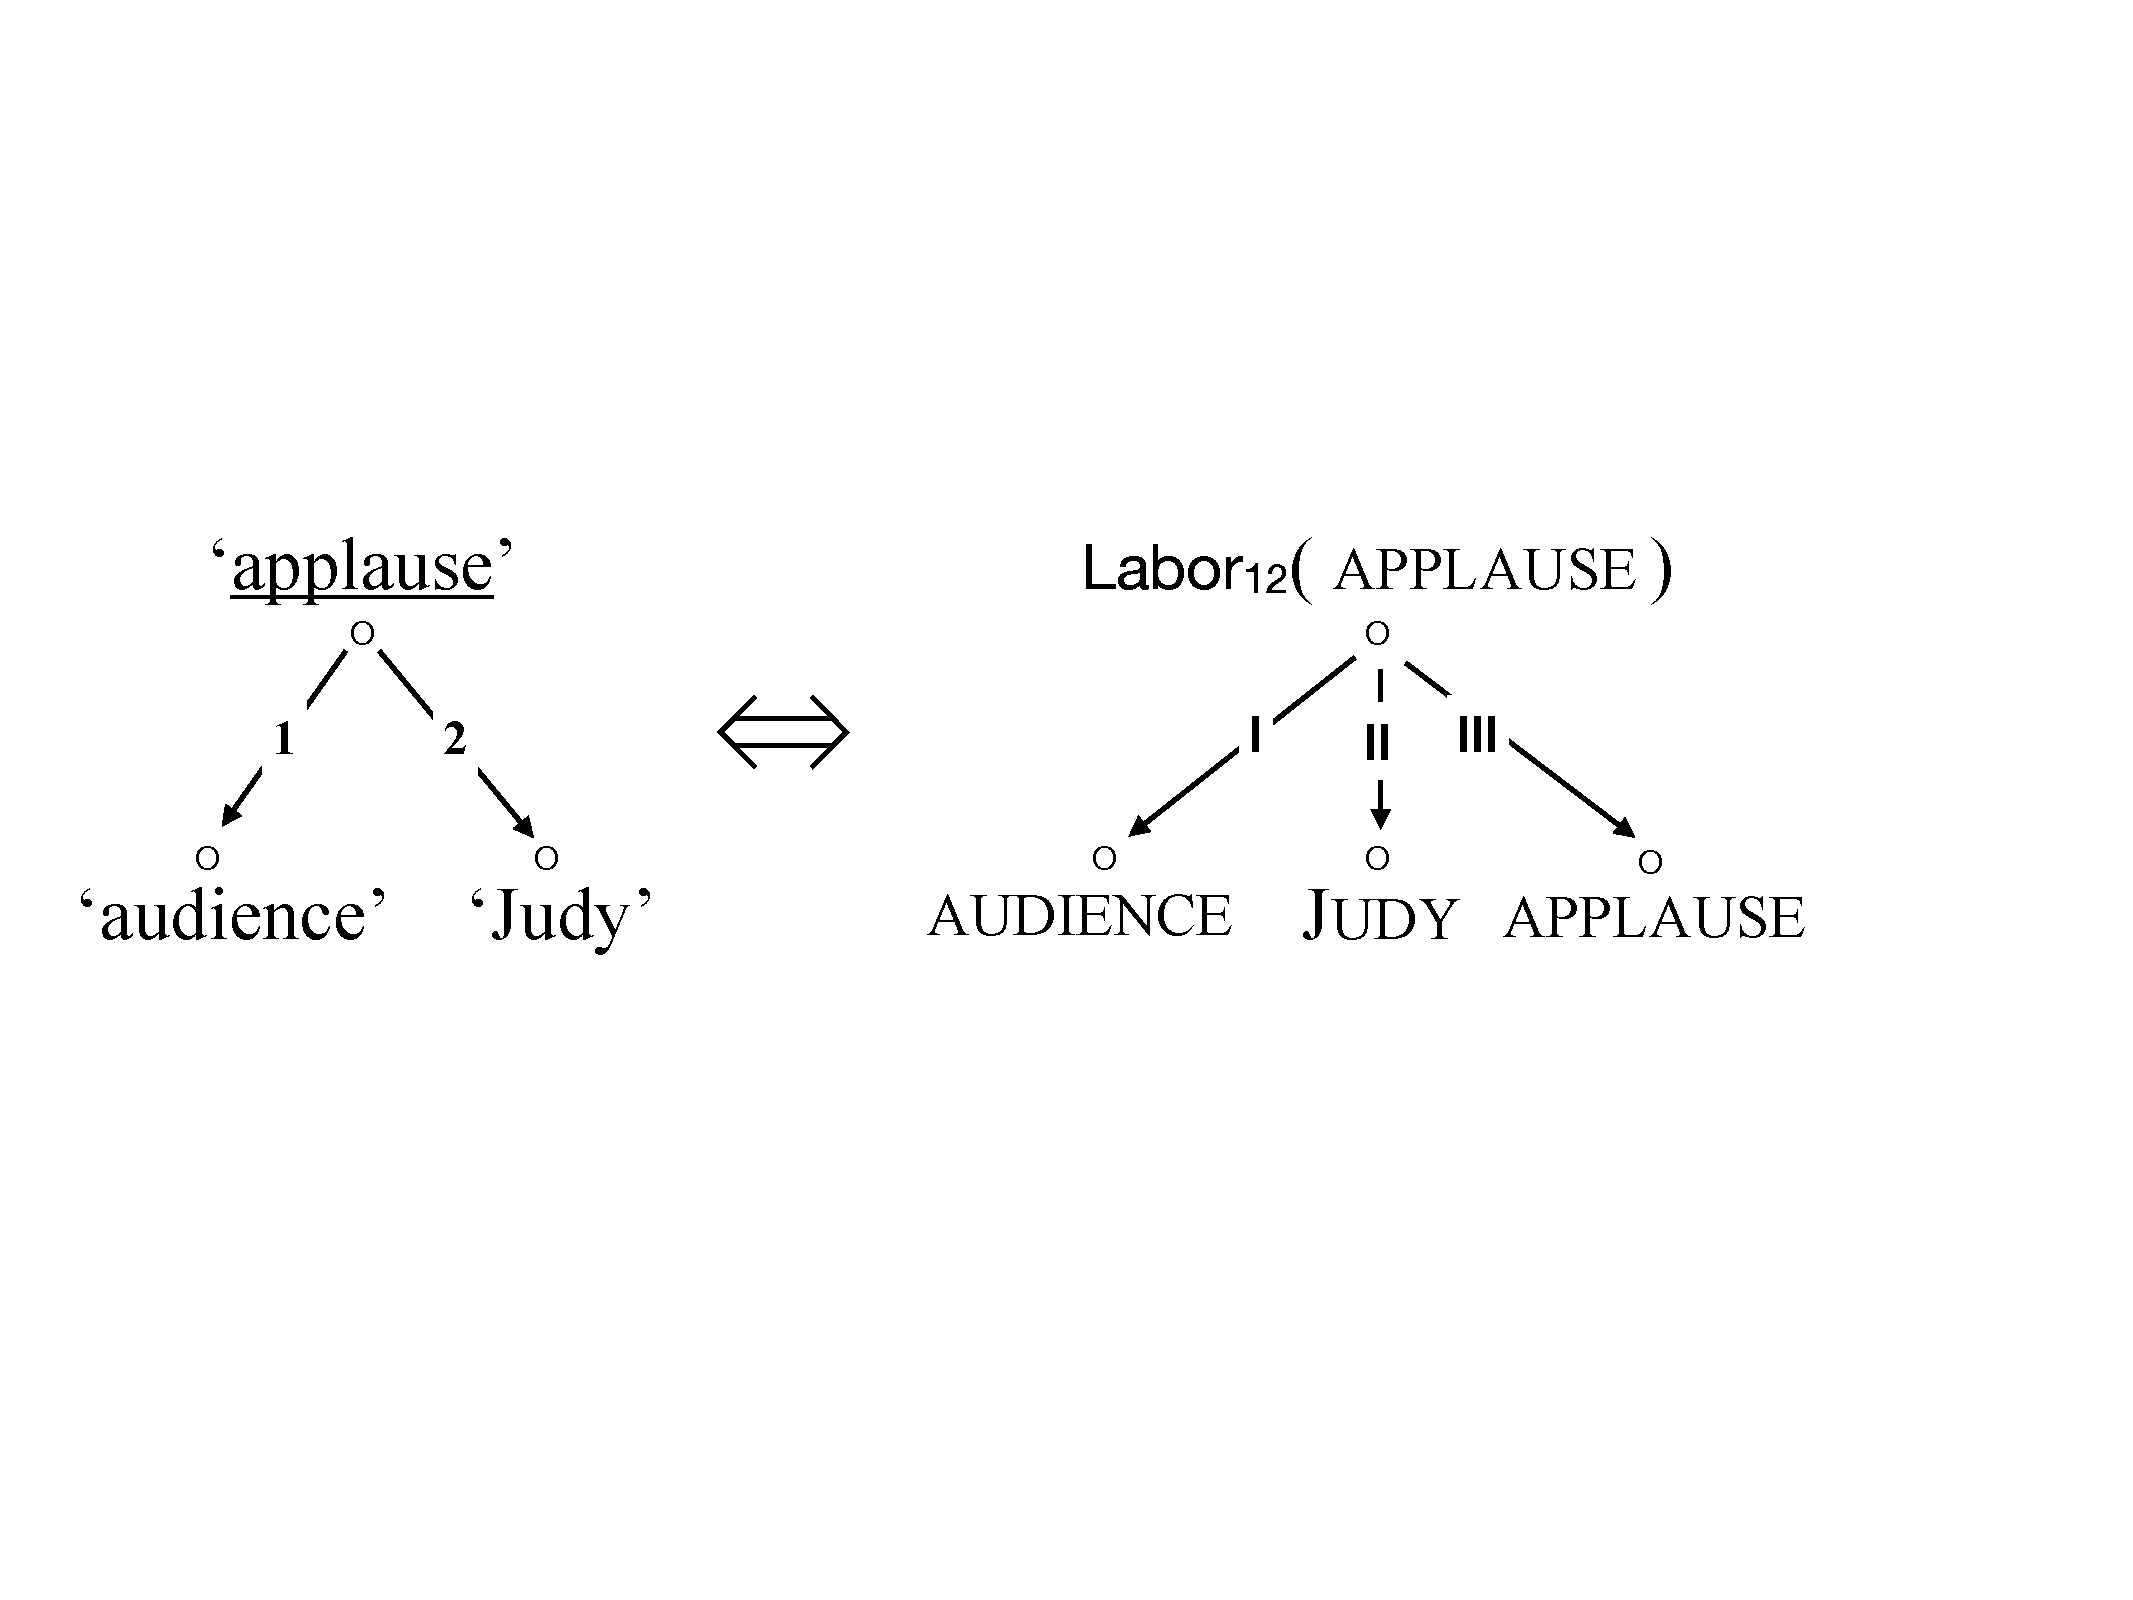
\includegraphics[width=0.65\linewidth]{Fig/SyntLF/SemSyntLabor-ij-illustr.pdf}
\caption{\lf{Labor\tsub{12}} in the Sem\thinspace$\Leftrightarrow$\thinspace{}DSynt correspondence with L~= \mbox{\textsc{applause}}}\label{fig:Labor-ij-illustr}
\end{figure}

The DSynt-structure given in \figref{fig:Labor-ij-illustr} is expressed by sentence \Next:

\begingroup
\small

\ex. The audience \emph{meets} Judy with applause.

\endgroup

\begin{longtable*}[l]{ l l >{\raggedright\arraybackslash}p{5cm} }

\multicolumn{3}{l}{\textbf{English}} \\*

\lfappl{Labor\tsub{12}}{\textit{esteem}\tsub{(N)} \lfgp{\textit{of} N\tsub{X} \textit{for} N\tsub{Y}}} & = & \textit{hold} \lfgp{N\tsub{Y} \textit{in} \tld} \\
\lfappl{Labor\tsub{12}}{\textit{use}\tsub{(N)} \lfgp{\textit{by} N\tsub{X} \textit{of} N\tsub{Y}}} & = & \textit{put} \lfgp{N\tsub{Y} \textit{to} \tld} \\
\lfappl{Labor\tsub{21}}{\lfgp{N\tsub{X},} \textit{result}\tsub{(N)} \lfgp{\textit{of} N\tsub{Y}}} & = & \textit{have} \lfgp{N\tsub{X} \textit{as a} \tld} \\[6pt]

\multicolumn{3}{l}{\textbf{French}} \\*

\lfappl{Labor\tsub{12}}{\textit{estime} \lfgp{\textit{de} N\tsub{X} \textit{pour}  N\tsub{Y}}} & = & \textit{avoir}\textbf{,} \textit{tenir} \lfgp{N\tsub{Y} \textit{en} \tld}\\
\lfappl{Labor\tsub{12}}{\textit{soins} \lfgp{\textit{de} N\tsub{X} \textit{destinés à}  N\tsub{Y}}} & = & \textit{entourer} \lfgp{N\tsub{Y} \textit{de} \tld}\\
\lfappl{Labor\tsub{21}}{\lfgp{N\tsub{X},} \textit{résultat} \lfgp{\textit{de} N\tsub{Y}}} & = & \textit{avoir} \lfgp{N\tsub{X} \textit{comme} \tld} \\[6pt]

\multicolumn{3}{l}{\textbf{Russian}} \\*

\lfappl{Labor\tsub{12}}{\textit{vlast\suffixsplit{}\palati} \lfgp{N\tsub{X-\textsc{gen}} \textit{nad} N\tsub{Y-\textsc{instr}}}} & = & \textit{der\v{z}at\palati} \lfgp{N\tsub{\textsc{acc}} \textit{pod} (\textit{svoej}) \tld\palat\textit{ju}} \\
\lfappl{Labor\tsub{12}}{\textit{zabot\suffixsplit{}a} \lfgp{N\tsub{X-\textsc{gen}} \textit{o} N\tsub{Y-\textsc{prepos}}}} & = & \textit{okru\v{z}it\palati} \lfgp{N\tsub{Y-\textsc{acc}} \tld\textit{oj}} \\*
\lfappl{Labor\tsub{21}}{\lfgp{N\tsub{X-\textsc{nom}},} \textit{rezul\palati{}tat} \lfgp{N\tsub{Y-\textsc{gen}}}} & = & \textit{imet\palati} \lfgp{N\tsub{X-\textsc{acc}} \tld\textit{om} $\langle$\textit{v ka\v{c}estve} \tld\textit{a}$\rangle$} \\

\end{longtable*}

\figref{fig:Labor-ij} and the above illustrations describe the prototypical case, where the argument L of \lf{Labor\tsub{ij}} is  bi-actantial. In such a case, \lfappl{Labor\tsub{ij}}{L} governs three \mbox{DSyntAs}, L filling the most oblique DSynt-slot. However, there are Ls with more than two DSyntAs. As a result of the transfer\index[notion]{actant!transfer of deep-syntactic \tld}\footnote{That is, syntactic raising -- see above, ``\nameref*{par:transferOfLsActants},'' p.\thinspace\pageref{par:transferOfLsActants}.}\index[notion]{raising, syntactic} of L's DSyntAs to the support verb, one obtains \lf{Labor} verbs with more than three DSyntAs. Take, for instance, the noun \textsc{inheritance} `belongings Y that X inherits from Z', and its French and Russian counterparts: they control three four-actantial \lf{Labor} collocates, as illustrated below.

\begin{longtable*}[l]{ l l >{\raggedright\arraybackslash}p{7cm} }

\multicolumn{3}{l}{\textbf{English}} \\*

\lfappl{Labor\tsub{123}}{\textit{inheritance}} & = & \textit{receive} \lfgp{N\tsub{Y$\Leftrightarrow${\tiny \textsf{\textbf{II}}}} \textit{from} N\tsub{Z$\Leftrightarrow${\tiny \textsf{\textbf{III}}}} \textit{as} \tld\tsub{L$\Leftrightarrow${\tiny \textsf{\textbf{IV}}}}} \\
\lfappl{Labor\tsub{321}}{\textit{inheritance}} & = & \textit{leave}\tsub{(V)} \lfgp{N\tsub{Y$\Leftrightarrow${\tiny \textsf{\textbf{II}}}} \textit{to} N\tsub{X$\Leftrightarrow${\tiny \textsf{\textbf{III}}}} \textit{as} \tld\tsub{L$\Leftrightarrow${\tiny \textsf{\textbf{IV}}}}} \\
\lfappl{Labor\tsub{213}}{\textit{inheritance}} & = & \textit{come}\tsub{(V)} \lfgp{\textit{to} N\tsub{X$\Leftrightarrow${\tiny \textsf{\textbf{II}}}} \textit{from} N\tsub{Z$\Leftrightarrow${\tiny \textsf{\textbf{III}}}} \textit{as} \tld\tsub{L$\Leftrightarrow${\tiny \textsf{\textbf{IV}}}}} \\[6pt]

\multicolumn{3}{l}{\textbf{French}} \\*

\lfappl{Labor\tsub{123}}{\textit{héritage}} & = & \textit{obtenir}\textbf{,} \textit{recevoir} \lfgp{N\tsub{Y$\Leftrightarrow${\tiny \textsf{\textbf{II}}}} \textit{de} N\tsub{Z$\Leftrightarrow${\tiny \textsf{\textbf{III}}}} \textit{en} \tld\tsub{L$\Leftrightarrow${\tiny \textsf{\textbf{IV}}}}}\\
\lfappl{Labor\tsub{321}}{\textit{héritage}} & = & \textit{laisser}\textbf{,} \textit{léguer} \lfgp{N\tsub{Y$\Leftrightarrow${\tiny \textsf{\textbf{II}}}} \textit{à} N\tsub{X$\Leftrightarrow${\tiny \textsf{\textbf{III}}}} \textit{en} \tld\tsub{L$\Leftrightarrow${\tiny \textsf{\textbf{IV}}}}} \\
\lfappl{Labor\tsub{213}}{\textit{héritage}} & = & \uslabel{specialized} \textit{échoir}\textbf{,} \textit{venir} \lfgp{\textit{à} N\tsub{X$\Leftrightarrow${\tiny \textsf{\textbf{II}}}} \textit{de} N\tsub{Z$\Leftrightarrow${\tiny \textsf{\textbf{III}}}} \textit{en} \tld\tsub{L$\Leftrightarrow${\tiny \textsf{\textbf{IV}}}}} \\[6pt]

\multicolumn{3}{l}{\textbf{Russian}} \\*

\lfappl{Labor\tsub{123}}{\textit{nasledstv\suffixsplit{}o}} & = & \textit{polu\v{c}it\palati} \lfgp{N\tsub{-\textsc{acc} Y$\Leftrightarrow${\tiny \textsf{\textbf{II}}}} \textit{ot} N\tsub{-\textsc{gen} Z$\Leftrightarrow${\tiny \textsf{\textbf{III}}}} \textit{v}\sensenum{2} \tld\textit{o}\tsub{L$\Leftrightarrow${\tiny \textsf{\textbf{IV}}}}}\\
\lfappl{Labor\tsub{321}}{\textit{nasledstv\suffixsplit{}o}} & = & \textit{ostavit\palati} \lfgp{N\tsub{-\textsc{acc} Y$\Leftrightarrow${\tiny \textsf{\textbf{II}}}} N\tsub{-\textsc{dat} X$\Leftrightarrow${\tiny \textsf{\textbf{III}}}} \textit{v}\sensenum{2} \tld\textit{o}\tsub{L$\Leftrightarrow${\tiny \textsf{\textbf{IV}}}}} \\
\lfappl{Labor\tsub{213}}{\textit{nasledstv\suffixsplit{}o}} & = & \textit{dostat\palati{}sja} \lfgp{N\tsub{-\textsc{dat} X$\Leftrightarrow${\tiny \textsf{\textbf{II}}}} \textit{ot} N\tsub{-\textsc{gen} Z$\Leftrightarrow${\tiny \textsf{\textbf{III}}}} \textit{v}\sensenum{2} \tld\textit{o}\tsub{L$\Leftrightarrow${\tiny \textsf{\textbf{IV}}}}} \\

\end{longtable*}

As we have seen, a collocational support verb \lf{Labor\tsub{ij}} relegates the collocation's base L  to the most oblique syntactic role: thus, L occupies the least privileged syntactic position, and this is anti-iconic\index[notion]{iconicity}. As a consequence, cases of \lf{Labor\tsub{ij}} are the least frequent ones among support verbs.

It is important to emphasize that the three support verb LFs are syntactically conversive\index[notion]{conversive} to each other, so that \lfappl{Func\tsub{1}}{L} $=$ \lfappl{Conv\tsub{21}Oper\tsub{1}}{L}, etc.:

\begingroup
\small

\ex. \a. \begingroup\setlength{\tabcolsep}{2pt}
\begin{tabular}[t]{ >{\raggedright\arraybackslash}p{2.6cm} c >{\raggedright\arraybackslash}p{7cm} }
\lfappl{Oper\tsub{1}}{\textit{analysis}} & = & \idiom{\textit{carry out}}\textbf{,} \textit{conduct}\tsub{(V)}\textbf{,} \textit{make}\tsub{(V)} \lfgp{\textsc{art} \tld} \\
\lfappl{Oper\tsub{2}}{\textit{analysis}} & = & \textit{undergo} \lfgp{\textsc{art} \tld} \\
\end{tabular}\endgroup
\b. \begingroup\setlength{\tabcolsep}{2pt}
\begin{tabular}[t]{ >{\raggedright\arraybackslash}p{2.6cm} c >{\raggedright\arraybackslash}p{7cm} }
\lfappl{Func\tsub{1}}{\textit{analysis}} & = & \textit{come}\tsub{(V)} \lfgp{\textit{from} N\tsub{X}} \\
\lfappl{Func\tsub{2}}{\textit{analysis}} & = & \textit{concern}\tsub{(V)} \lfgp{N\tsub{Y}} \\
\end{tabular}\endgroup
\c. \begingroup\setlength{\tabcolsep}{2pt}
\begin{tabular}[t]{ >{\raggedright\arraybackslash}p{2.6cm} c >{\raggedright\arraybackslash}p{7cm} }
\lfappl{Labor\tsub{12}}{\textit{analysis}} & = & \textit{subject}\tsub{(V)} \lfgp{N\tsub{Y} \textit{to} \textsc{art} \tld} \\
\end{tabular}\endgroup

\endgroup

To round off the present section, we will consider three cases of support verb\index[notion]{support verb!\tld\ with non-nominal base}\index[notion]{verb!support \tld\ with non-nominal base} collocations having a non-nominal base.

\begin{enumerate}

\item In SAE languages\index[notion]{Standard Average European [SAE] language}, all adjectives\index[notion]{adjective!\tld's support verb} used as attributive complement of a copula verb\index[notion]{copula verb}\index[notion]{verb!copula \tld} have the same ``joker''\index[notion]{value of an LF!joker \tld}\index[notion]{joker value of an LF}\index[notion]{lexical function!joker value of a \tld} \lf{Oper\tsub{1}}\index[lf]{Operi@\lf{Oper\tsub{i}}!joker \lf{Oper\tsub{1}}} support verb; for English, French and Russian: \textsc{be}\tsub{(copula)}\index[notion]{copula verb}\index[notion]{verb!copula \tld}, \textsc{être}\tsub{(copula)} and \textsc{byt\palat}\tsub{(copula)}.

\lfappl{Oper\tsub{1}}{L\tsub{(Adj)}} is equivalent to \lfappl{Copul}{L\tsub{(Adj)}}\index[lf]{Copul@\lf{Copul}} -- \sectref{sec:verbeCopule}, [\ref{lf:Copul}], p.\thinspace\pageref{lf:Copul}. Since the corresponding phrases are free (non-phraseologized), they are not to be considered here.

\item However, adjectives and adverbs denoting meteorological phenomena behave differently. They have a specific \lf{Oper\tsub{i}}: an impersonal \lf{Oper\tsub{0}}\index[notion]{verb!impersonal \tld}\index[notion]{impersonal verb}\index[lf]{Operi@\lf{Oper\tsub{i}}!\lf{Oper\tsub{0}}}.

\begin{longtable*}{ l l >{\raggedright\arraybackslash}p{6.5cm} }

\multicolumn{3}{l}{\textbf{English}} \\*

\lfappl{Oper\tsub{0}}{\textit{hot}\slashs\textit{misty}} & = & \lfgp{\textit{it}\tsub{(impers)}} \textit{be}\tsub{(meteo)} \lfgp{\tld} \\*
& & {\small\textit{It was hot}\thinspace/\thinspace\textit{misty in Montreal.}} \\[3pt]

\multicolumn{3}{l}{\textbf{French}} \\*

\lfappl{Oper\tsub{0}}{\textit{chaud}} & = & \lfgp{\textit{il}\tsub{(impers)}} \textit{faire}\tsub{(meteo)} \lfgp{\tld}\\
& & {\small\textit{Il faisait chaud à Montréal.}} \\
\lfappl{Oper\tsub{0}}{\textit{brumeux}} & = & \lfgp{\textit{il}\tsub{(impers)}} \textit{faire}\tsub{(meteo)}\textbf{,} \lfgp{\textit{ce}\tsub{(impers)}} \textit{être}\tsub{(meteo)} \lfgp{\tld} \\*
& & {\small\textit{Il faisait} $\langle$\textit{C'était}$\rangle$ \textit{brumeux à Montréal.}} \\[3pt]

\multicolumn{3}{l}{\textbf{Russian}} \\*

\lfappl{Oper\tsub{0}}{\textit{\v{z}arko}\slashs\textit{tumanno}} & = & \lfgp{Ø\tsub{(impers)}} \textit{byt\palati}\tsub{(meteo)} \lfgp{\tld} \\
& & {\small\textit{V Monreale bylo \v{z}arko{\upshape \slashs}tumanno.}} \vspace{6pt} \\

\end{longtable*}

\item \idiom{Prep\thinspace$\rightarrow$\thinspace{}N} adverbial idioms having several \lf{Oper\tsub{1}} collocates are not uncommon, as illustrated by the English idiom \idiom{\textsc{on cloud nine}} `extremely happy':\footnote{See also \textcite[136]{MelcukPolguere2021} for a detailed analysis of the French idiom  \idiom{\textsc{dans la semoule}} (lit.~`in the semolina') `not knowing what to do in a difficult situation' and its \lf{Oper\tsub{1}} collocates: \textit{être} `be', \textit{nager} `swim', \textit{patauger} `wade' and \textit{pédaler} `pedal'.}

\begingroup
\small

\ex. \begingroup\setlength{\tabcolsep}{2pt}
\begin{tabular}[t]{ l l >{\raggedright\arraybackslash}p{7cm} }
\lfappl{Oper\tsub{1}}{\idiom{\textit{on cloud nine}}} & = & \textit{be}\textbf{,} \textit{float}\tsub{(V)}\textbf{,} \textit{fly}\tsub{(V)} \lfgp{\tld} \\
\end{tabular}\endgroup

\endgroup

\end{enumerate}

\subsection{Realization verbs}\label{sec:verbeReal}

\index[notion]{realization verb|emph}\index[notion]{verb!realization \tld|emph}This section introduces three types of verbal collocates that are similar in their syntactic behavior to the three support verbs described in the previous section. Semantically, however, \notion{realization verbs} are very different. They are not empty, but express a specific meaning: `fulfill an inherent requirement of L' -- in the most general sense (more specifically, `realize', `use', `accomplish', etc.). This semantic load justifies the name \emph{realization verbs}. Just as the support verb LFs, the three realization verb LFs are mutual conversives\index[notion]{conversive}.

A fourth LF that is semantically related to realization verb LFs is also introduced at the end of this section: \lf{Prepar}. It is, so to speak, a realization verb by extension.

All four verbal LFs presented in this section have the same PoS table:

\begin{quote}
\begingroup
\phantomsection\label{tab:PdDVReal}\small
\begin{tabular}{ l c c }
   \midrule
   \multicolumn{3}{l}{\lf{Real\tsub{i}}, \lf{Fact\tsub{i}}, \lf{Labreal\tsub{ij}}, \lf{Prepar}: verbal} \\
   \midrule
   \textbf{L} & \cellcolor[gray]{0.85}V & N \\
   \midrule
\textbf{\lfappl{Real\tsub{i}\slashs{}Fact\tsub{i}\slashs{}Labreal\tsub{ij}\slashs{}Prepar}{L}} & \cellcolor[gray]{0.85}V & V \\
   \midrule
\end{tabular}
\endgroup
\end{quote}

This table shows that the realization verbs prototypically have a nominal base. The shading of the column for verbal bases indicates that these cases present some complications -- see ``\nameref*{par:RealVFusion}'' below, p.\thinspace\pageref{par:RealVFusion}.

\refstepcounter{LFlist}
\subsubsection*{{\small [\arabic{LFlist}]} \lf{Real\tsub{i}} \lfgp{{\scriptsize Latin} \textit{realis} `real'}
: realization verb that means `fulfill [L]'} \label{lf:Real-i}
\addcontentsline{toc}{subsection}{{\footnotesize [\arabic{LFlist}]} \lf{Real\tsub{i}}: realization verb that means `fulfill \lfgp{L}'}\index[lf]{Reali@\lf{Real\tsub{i}}|emph}

\lfappl{Real\tsub{i}}{L} is a realization verb that takes L as DSyntA\thinspace\syntDname{II} and the DSyntA\thinspace\syntDname{i} of L as DSyntA\thinspace\syntDname{I}. It controls the same syntactic structure as support verbs of the type \lf{Oper\tsub{i}}\index[lf]{Operi@\lf{Oper\tsub{i}}}.

\begin{longtable*}[l]{ l l >{\raggedright\arraybackslash}p{6cm} }

\multicolumn{3}{l}{\textbf{English}} \\*

\lfappl{Real\tsub{1}}{\textit{promise}\tsub{(N)}} & = & \textit{keep} \lfgp{\textsc{art} \tld} \\
\lfappl{Real\tsub{2}}{\textit{expectations}} & = & \idiom{\textit{come up}} \lfgp{\textit{to} \textsc{art} \tld}\textbf{,} \textit{fulfill} \lfgp{\textsc{art} \tld}\textbf{;} \idiom{\textit{live up}} \lfgp{\textit{to} \textsc{art} \tld} \\
\lfappl{Real\tsub{3}}{\textit{order}\tsub{(N)}} & = & \idiom{\textit{carry out}}\textbf{,} \textit{execute}\textbf{,} \textit{fulfill} \lfgp{\textsc{art} \tld} \\
\multicolumn{3}{l}{\quad\lfgp{N\tsub{X}\textit{'s order to} V\tsub{Y} \textit{to} N\tsub{Z}}} \\
\lfappl{Real\tsub{1}}{\textit{plane}\tsub{(N)}} & = & \textit{pilot}\tsub{(V)} \lfgp{\textsc{art} \tld} \\[6pt]

\multicolumn{3}{l}{\textbf{French}} \\*

\lfappl{Real\tsub{1}}{\textit{promesse}} & = & \textit{tenir} \lfgp{\textsc{art} \tld}\\
\lfappl{Real\tsub{2}}{\textit{attentes}} & = & \textit{répondre} \lfgp{\textit{à} \textsc{art} \tld}\\
\lfappl{Real\tsub{3}}{\textit{ordre}} & = & \textit{exécuter}\textbf{,} \textit{suivre} \lfgp{\textsc{art} \tld}\\
\multicolumn{3}{l}{\quad\lfgp{\textit{ordre de} N\tsub{X} \textit{de} V\tsub{Y-\textsc{inf}} \textit{à} N\tsub{Z}}} \\
\lfappl{Real\tsub{1}}{\textit{avion}} & = & \textit{piloter} \lfgp{\textsc{art} \tld}\\
\lfappl{Real\tsub{1}}{\idiom{\textit{chasse d'eau}}} & = & \textit{actionner}\textbf{,} \textit{activer}\textbf{,} \textit{tirer} \lfgp{\textsc{art} \tld} \\[6pt]

\multicolumn{3}{l}{\textbf{Russian}} \\*

\lfappl{Real\tsub{1}}{\textit{obe\v{s}\v{c}ani\suffixsplit{}e}} & = & \textit{sder\v{z}at\palati}\textbf{,} \textit{vypolnit\palati} \lfgp{ \tld\textit{e}} \\
\lfappl{Real\tsub{2}}{\textit{ožidani\suffixsplit{}ja}} & = & \textit{opravdat\palati} \lfgp{\tld\textit{ja}} \\
\lfappl{Real\tsub{3}}{\textit{prikaz}} & = & \textit{vypolnit\palati} \lfgp{\tld} \\*
\multicolumn{3}{l}{\quad\lfgp{\textit{prikaz} N\tsub{X-\textsc{gen}} V\tsub{Y-\textsc{inf}} N\tsub{Z-\textsc{dat}}}} \\*
\lfappl{Real\tsub{1}}{\textit{samolët}} & = & \textit{pilotirovat\palati}\textbf{,} \textit{vesti} \lfgp{\tld} \\

\end{longtable*}

The argument L of \lf{Real\tsub{i}} -- just as of the two other realization verbs -- must contain in its lexicographic definition\index[notion]{definition!lexicographic \tld} at least one particular semantic component which expresses a ``requirement'' of L and thus is compatible with the meaning of realization. It is this component that is the target\index[notion]{target of an LF}\index[notion]{lexical function!target of a \tld} for \lf{Real\tsub{i}}.\footnote{See the presentation of targets of LFs in \chapref{chap:NotionLF}, \sectref{sec:classeFLSyntagmatiques}, p.\thinspace\pageref{txt:targetOfSyntLF}.} Consider, for instance, the definition of the noun \textsc{debt}:

\begingroup
\small

\ex. \label{ldef:defDEBT}\APolbox{9.3cm}{%
   \begin{tabular}{ l p{5.6cm} }
   \textit{X's debt of Y to Z} :
   &
   sum of money Y that X got from Z \newline
   \setlength{\tabcolsep}{.5pt}\begin{tabular}{ p{0.2cm} >{\raggedright\arraybackslash}p{5.3cm} }
   \SpecDiff &  that X \emph{is expected to \idiom{pay back}} to Z \\
   \end{tabular} \\
\end{tabular}
}

\endgroup

The emphasized component (`is expected to \idiom{pay back}') corresponds to the inherent requirement of \textsc{debt}, which is targeted
in the \lf{Real\tsub{1}} collocations: \textit{clear}, \idiom{\textit{pay back}}, \idiom{\textit{pay off}}, \textit{repay a debt}.

\paragraph*{Degree of realization.}\label{par:degreesOfReal}

The elements of the value of \lfappl{Real\tsub{i}}{L} may differ by the degree of realization\index[notion]{degree of realization}. Three degrees are distinguished, using the superscripts \lf{\tsup{I}}, \lf{\tsup{II}} and \lf{\tsup{III}}\index[lf]{Reali@\lf{Real\tsub{i}}!\lf{Real\tsub{1}}@\lf{Real$_\text{1}^\text{I}$}|emph}:

\begingroup
\small

\ex. \a. \begingroup\setlength{\tabcolsep}{2pt}
\begin{tabular}[t]{ l l >{\raggedright\arraybackslash}p{7cm} }
\lfappl{Real$_\text{1}^\text{I}$}{\textit{suitcase}} & = & \textit{fill}\tsub{(V)}\textbf{,} \textit{pack}\tsub{(V)} \lfgp{\textsc{art} \tld} \\
\lfappl{Real$_\text{1}^\text{II}$}{\textit{suitcase}} & = & \textit{carry}\tsub{(V)} \lfgp{\textsc{art} \tld}\textbf{;} \textit{drag}\tsub{(V)} \lfgp{\textsc{art} \tld}\textbf{;} \textit{wheel}\tsub{(V)} \lfgp{\textsc{art} \tld} \\
\lfappl{Real$_\text{1}^\text{III}$}{\textit{suitcase}} & = & \textit{empty}\tsub{(V)}\textbf{,} \textit{unpack} \lfgp{\textsc{art} \tld} \\
\end{tabular}\endgroup
\b. \begingroup\setlength{\tabcolsep}{2pt}
\begin{tabular}[t]{ l l >{\raggedright\arraybackslash}p{7cm} }
\lfappl{Real$_\text{2}^\text{I}$}{\textit{task}\tsub{(N)}} & = & \textit{tackle}\tsub{(V)} \lfgp{\textsc{art} \tld} \\
\lfappl{Real$_\text{2}^\text{II}$}{\textit{task}\tsub{(N)}} & = & \textit{fulfill} \lfgp{\textsc{art} \tld} \\
\end{tabular}\endgroup
%\lfappl{Real\textsubscript{\raisebox{-1pt}{\rlap{2}}}\textsuperscript{\raisebox{1pt}{I}}}{\textit{peine} \lfgp{jurid.}} & = & \textit{recevoir} \lfgp{\textsc{art} \tld}\\
%\lfappl{Real\textsubscript{\raisebox{-1pt}{\rlap{2}}}\textsuperscript{\raisebox{1pt}{II}}}{\textit{peine} \lfgp{jurid.}} & = & \textit{purger} \lfgp{\textsc{art} \tld}\\
%\lfappl{Real\textsubscript{\raisebox{-1pt}{\rlap{2}}}\textsuperscript{\raisebox{1pt}{I}}}{\textit{livre}} & = & \textit{ouvrir} \lfgp{\textsc{art} \tld}\\
%\lfappl{Real\textsubscript{\raisebox{-1pt}{\rlap{2}}}\textsuperscript{\raisebox{1pt}{II}}}{\textit{livre}} & = & \textit{lire} \lfgp{\textsc{art} \tld}\\

\endgroup

Some details on the distinction between \lf{Real$_\text{i}^\text{I}$} and the LF \lf{Prepar}\index[lf]{Prepar@\lf{Prepar}} are given below ([\ref{lf:Prepar}], p.\thinspace\pageref{it:diffPreparReal1--I}).

\paragraph*{External participant as realizer.}\label{par:RealOmega}

The ``realizer'' of \lfappl{Real\tsub{i}}{L} can be an external participant\index[notion]{participant of a situation!external \tld} of the situation denoted by L  (cf. \chapref{chap:preliminaryNotions}, \sectref{sec:semanticNotions}, p.\thinspace\pageref{par:externalParticipant}). In such cases, a special actantial subscript\index[notion]{actantial subscript!\tld\ \textOmega} \textOmega\ is used: \lf{Real\tsub{\textOmega}}\index[lf]{Reali@\lf{Real\tsub{i}}!\lf{Real\tsub{\textOmega}}|emph}. The symbol \textOmega\ indicates that the DSyntA\thinspace\syntDname{I} of \lfappl{Real\tsub{\textOmega}}{L} does not correspond to one of L's DSyntAs. Here are a few illustrations:

\begingroup
\small

\ex. \begingroup\setlength{\tabcolsep}{2pt}
\begin{tabular}[t]{ l l >{\raggedright\arraybackslash}p{7cm} }
\lfappl{Real\tsub{\textOmega}}{\textit{mountain}} & = &  \textit{climb}\tsub{(V)}\textbf{,} \textit{scale}\tsub{(V)} \lfgp{\textsc{art} \tld} \\
\lfappl{Real\tsub{\textOmega}}{\textit{costs}\tsub{(N)}} & = &  \textit{cover}\tsub{(V)} \lfgp{\textsc{art} \tld} \\
\lfappl{Real\tsub{\textOmega}}{\textit{baby}\tsub{(N)}} & = & \idiom{\textit{take care}} \lfgp{\textit{of} \textsc{art} \tld}\textbf{,} \fused\textit{babysit} \\
\lfappl{Real\tsub{\textOmega}}{\textit{pulse}\tsub{(N)}} & = & \textit{feel}\tsub{(V)}\textbf{,} \textit{take}\tsub{(V)} \lfgp{\textsc{art} \tld} \\
%\lfappl{Real\tsub{\textOmega}}{\textit{épidémie}} & = & \textit{combattre} \lfgp{\textsc{art} \tld}\textbf{,} \textit{lutter} \lfgp{\textit{contre} \textsc{art} \tld}\\
%\lfappl{Real\tsub{\textOmega}}{\textit{dette}} & = & \idiom{\textit{prendre en charge}} \lfgp{\textsc{art} \tld}\\
%\lfappl{Real\tsub{\textOmega}}{\textit{bébé}} & = & \textit{s'occuper} \lfgp{\textit{de} \textsc{art} \tld}\textbf{;} \textit{garder} \lfgp{\textsc{art} \tld}\\
%\lfappl{Real\tsub{\textOmega}}{\textit{pouls}} & = & \textit{prendre} \lfgp{\textsc{art} \tld\ \textit{à} N\tsub{X}}\textbf{,} \textit{tâter} \lfgp{\textsc{art} \tld}\\
\end{tabular}\endgroup

\endgroup

\begin{historicalremark}
In previous lexicographic projects -- in particular, in the development of the \notion{DiCo} lexical database \parencite{Polguere2000b} --, subscripts $\lozenge$ or @ have been used in place of \textOmega.
\end{historicalremark}\index[notion]{lexical database!DiCo}\index[notion]{DiCo}

\paragraph*{Verbal argument of \lf{Real\tsub{i}}.}\label{par:RealVFusion}

\lf{Real\tsub{i}} can also apply to a verb. In this case, \lfappl{Real\tsub{i}}{L} normally gives fused\index[notion]{fusion}\index[notion]{value of an LF!fused \tld} values:

\begingroup
\small

\ex. \begingroup\setlength{\tabcolsep}{2pt}
\begin{tabular}[t]{ l l >{\raggedright\arraybackslash}p{7cm} }
\lfappl{Real\tsub{1}}{\textit{approach}\tsub{(V)} \lfgp{N\tsub{Y}}} & = & \fused\textit{reach}\tsub{(V)} \lfgp{N\tsub{Y}} \\
\lfappl{Real\tsub{1}}{\textit{look}\tsub{(V)} \lfgp{for N\tsub{Y}}} & = & \fused\textit{find}\tsub{(V)} \lfgp{N\tsub{Y}} \\
\lfappl{Real\tsub{1}}{\textit{pursue} \lfgp{N\tsub{Y}}} & = & \fused\textit{catch}\tsub{(V)} \lfgp{N\tsub{Y}} \\
\lfappl{Real\tsub{1}}{\textit{stagger}\tsub{(V)}} & = & \fused\textit{fall}\tsub{(V)} \\
\lfappl{Real\tsub{2}}{\textit{rock}\tsub{(V)} \lfgp{N\tsub{Y}}} & = & \fused\textit{fall asleep} \\
%\lfappl{Real\tsub{1}}{\textit{s'approcher} \lfgp{\textit{de} N\tsub{Y}}} & = & \fused\textit{atteindre} \lfgp{N\tsub{Y}}\footnotemark \\
%\lfappl{Real\tsub{1}}{\textit{chercher}} & = & \fused\textit{trouver} \\
%\lfappl{Real\tsub{1}}{\textit{poursuivre}} & = & \fused\textit{attraper} \\
%\lfappl{Real\tsub{1}}{\textit{basculer}} & = & \fused\textit{tomber} \\
%\lfappl{Real\tsub{2}}{\textit{bercer}} & = & \fused\textit{s'endormir} \\
%Real1(približat´sja  [k NY]) =  dostič´ [NY-a]
%Real1(iskat´) = najti
%Real1(lovit´) = pojmat´
%Real1(pošatnut´sja) = upast´
%Real2(ukačivat´) = zasnut´
%\footnotetext{Comparer avec \lfappl{Result\tsub{1}}{\textit{atteindre} \lfgp{\textit{de} N\tsub{Y}}} = \textit{être} \lfgp{\lf{Loc\tsub{in}} N\tsub{Y}} -- \chapref{chap:paraLFs}, [\ref{lf:Result-i}], p.\thinspace\pageref{lf:Result-i}.}
\end{tabular}\endgroup

\endgroup

These fused \lfappl{Real\tsub{i}}{L} should not be mistaken for cases of \lfappl{Result\tsub{i}}{L}\index[lf]{Resulti@\lf{Result\tsub{i}}}, which are in a \emph{paradigmatic}\index[notion]{lexical function!paradigmatic vs. syntagmatic \tlds} relation with L (\chapref{chap:paraLFs}, [\ref{lf:Result-i}], p.\thinspace\pageref{lf:Result-i}). The situation denoted by \lfappl{Real\tsub{i}}{L}, contrary to \lfappl{Result\tsub{i}}{L}, is not necessarily a result of the situation denoted by L. For instance, one can fall asleep without being rocked -- cf. last illustration in \Last.

\paragraph*{Frequent combination with \lf{Anti}.}

Because it is not semantically empty, \lf{Real\tsub{i}} -- and the two other LFs of realization as well -- frequently combines with \lf{Anti}\index[lf]{Anti@\lf{Anti}}. As a result, \lfappl{AntiReal\tsub{i}}{L}\phantomsection\label{lf:AntiReal-i}\index[lf]{Reali@\lf{Real\tsub{i}}!\lf{AntiReal\tsub{i}}|emph} expresses the meaning `do the opposite of fulfilling an inherent requirement of~L'.

\begingroup
\small

\ex. \a. \begingroup\setlength{\tabcolsep}{2pt}
\begin{tabular}[t]{ >{\raggedright\arraybackslash}p{3.4cm} l >{\raggedright\arraybackslash}p{5cm} }
\lfappl{Real\tsub{1}}{\textit{impulse}\tsub{(N)}} & = & \textit{yield}\tsub{(V)} \lfgp{\textit{to} \textsc{art} \tld} \\*
\lfappl{AntiReal\tsub{1}}{\textit{impulse}\tsub{(N)}} & = & \textit{control}\tsub{(V)}\textbf{,} \textit{resist}\tsub{(V)} \lfgp{\textsc{art} \tld} \\
\end{tabular}\endgroup
\b. \begingroup\setlength{\tabcolsep}{2pt}
\begin{tabular}[t]{ >{\raggedright\arraybackslash}p{3.4cm} l >{\raggedright\arraybackslash}p{5cm} }
\lfappl{Real\tsub{1}}{\idiom{\textit{red light}}} & = & \textit{stop}\tsub{(V)} \lfgp{\textit{at} \textsc{art} \tld} \\*
\lfappl{AntiReal\tsub{1}}{\idiom{\textit{red light}}} & = & \textit{jump}\tsub{(V)}\textbf{,} \textit{run}\tsub{(V)} \lfgp{\textsc{art} \tld} \\
\end{tabular}\endgroup
\c. \begingroup\setlength{\tabcolsep}{2pt}
\begin{tabular}[t]{ >{\raggedright\arraybackslash}p{3.4cm} l >{\raggedright\arraybackslash}p{5cm} }
\lfappl{Real\tsub{2}}{\textit{exam}} & = & \textit{pass}\tsub{(V)} \lfgp{\textsc{art} \tld} \\*
\lfappl{AntiReal\tsub{2}}{\textit{exam}} & = & \textit{fail}\tsub{(V)} \lfgp{\textsc{art} \tld} \\
%\lfappl{Real\tsub{1}}{\textit{pulsion}} & = & \textit{céder} \lfgp{à \textsc{art} \tld} \\
%\lfappl{AntiReal\tsub{1}}{\textit{pulsion}} & = & \textit{contrôler} \lfgp{\textsc{art} \tld} \\
%\\
%\lfappl{Real\tsub{1}}{\idiom{\textit{feu rouge}}} & = & \textit{s'arrêter} \lfgp{à \textsc{art} \tld}\textbf{;} \\
 %& & \textit{respecter} \lfgp{\textsc{art} \tld} \\
%\lfappl{AntiReal\tsub{1}}{\idiom{\textit{feu rouge}}} & = & \textit{brûler}\textbf{,} \textit{griller} \lfgp{\textsc{art} \tld} \\
%\\
%\lfappl{Real\tsub{2}}{\textit{examen}} & = & \textit{réussir} \lfgp{\textsc{art} \tld} \\
%\lfappl{AntiReal\tsub{2}}{\textit{examen}} & = & \textit{échouer} \lfgp{\textit{à} \textsc{art} \tld} \\
\end{tabular}\endgroup

\endgroup

\refstepcounter{LFlist}
\subsubsection*{{\small [\arabic{LFlist}]} \lf{Fact\tsub{i}} \lfgp{{\scriptsize Latin} \textit{factum} `action, fact'}: realization verb that means `[L] be fulfilled'}\label{lf:Fact-i}
\addcontentsline{toc}{subsection}{{\footnotesize [\arabic{LFlist}]} \lf{Fact\tsub{i}}: realization verb that means `\lfgp{L} be fulfilled'}\index[lf]{Facti@\lf{Fact\tsub{i}}|emph}

\lfappl{Fact\tsub{i}}{L} is a realization verb that takes L as DSyntA\thinspace\syntDname{I} and the expression of the DSyntA\thinspace\syntDname{i} of L as DSyntA~\syntDname{II}.

This verb of realization is a conversive\index[notion]{conversive} of \lf{Real\tsub{i}}; it controls the same syntactic configuration as the support verb \lf{Func\tsub{i}}.

\phantomsection\label{txt:Fact0Descr}\lf{Fact\tsub{0}}\index[lf]{Facti@\lf{Fact\tsub{i}}!\lf{Fact\tsub{0}}|emph} (i.e., with \lf{i}~=~\lf{0}) means that the verbal collocate does not govern an object\index[notion]{object, syntactic} expressing a DSyntA of L.

\begin{longtable*}[l]{ l l >{\raggedright\arraybackslash}p{6cm} }

\multicolumn{3}{l}{\textbf{English}} \\*

\lfappl{Fact\tsub{0}}{\textit{dream}\tsub{(N)}} & = & \idiom{\textit{come true}}\\
\lfappl{Fact\tsub{1}}{\textit{fright}\tsub{(N)}} & = & \textit{paralyze} \lfgp{N\tsub{X}}\\
\lfappl{Fact\tsub{2}}{\textit{insolence}} & = & \textit{offend}\textbf{,} \textit{shock}\tsub{(V)} \lfgp{N\tsub{Y}} \\[6pt]

\multicolumn{3}{l}{\textbf{French}} \\*

\lfappl{Fact\tsub{0}}{\textit{rêve}} & = & \textit{se réaliser}\\
\lfappl{Fact\tsub{1}}{\textit{effroi}} & = & \textit{paralyser} \lfgp{N\tsub{X}}\\
\lfappl{Fact\tsub{2}}{\textit{insolence}} & = & \textit{choquer}\textbf{,} \textit{offenser}\textbf{,} \textit{offusquer} \lfgp{N\tsub{Y}} \\[6pt]

\multicolumn{3}{l}{\textbf{Russian}} \\*

\lfappl{Fact\tsub{0}}{\textit{me\v{c}ta}} & = & \textit{sbyt\palati{}sja} \\
\lfappl{Fact\tsub{1}}{\textit{u\v{z}as}} & = & \textit{paralizovat\palati} \lfgp{N\tsub{X-\textsc{acc}}} \\
\lfappl{Fact\tsub{2}}{\textit{naglost\palati}} & = & \textit{potrjasti}\textbf{,} \textit{vozmutit\palati} \lfgp{N\tsub{Y-\textsc{acc}}} \\

\end{longtable*}

\refstepcounter{LFlist}
\subsubsection*{{\small [\arabic{LFlist}]} \lf{Labreal\tsub{ij}} \lfgp{hybrid of \lf{Labor} and \lf{Real}}: realization verb that means `submit to the action [of L], thereby fulfilling [L]'}\label{lf:Labreal-ij}
\addcontentsline{toc}{subsection}{{\footnotesize [\arabic{LFlist}]} \lf{Labreal\tsub{ij}}: realization verb that means `submit to the action \lfgp{of~L}, thereby fulfilling \lfgp{L}'}\index[lf]{Labrealij@\lf{Labreal\tsub{ij}}|emph}

\lfappl{Labreal\tsub{ij}}{L} is a realization verb that takes L as its most oblique [=~most peripheral] DSyntA. Its DSyntA\thinspace\syntDname{I} corresponds to the DSyntA\thinspace\syntDname{i} of L and its DSyntA\thinspace\syntDname{II} corresponds to the DSyntA\thinspace\syntDname{j} of L. \lf{Labreal\tsub{ij}} controls the same syntactic configuration as support verbs of the \lf{Labor\tsub{ij}}\index[lf]{Laborij@\lf{Labor\tsub{ij}}} type.

The communicative\index[notion]{communicative!\tld\ information} effect of \lf{Labreal\tsub{ij}} is to give a peripheral position to the expression of L in the sentence, while communicatively favoring the expression of the actants \syntDname{i} and \syntDname{j}.

\begin{longtable*}[l]{ l l >{\raggedright\arraybackslash}p{6.6cm} }

\multicolumn{3}{l}{\textbf{English}} \\*

\lfappl{Labreal\tsub{12}}{\textit{microwave}\tsub{(N)}} & = & \textit{heat}\tsub{(V)} \lfgp{N\tsub{Y} \textit{in} \textsc{art} \tld}\textbf{,} \fused\textit{microwave}\tsub{(V)} \lfgp{N\tsub{Y}} \\
\lfappl{Labreal\tsub{12}}{\textit{trap}\tsub{(N)}} & = & \textit{catch}\tsub{(V)} \lfgp{N\tsub{Y} \textit{in} \textsc{art} \tld}\textbf{,} \fused\textit{trap}\tsub{(V)} \lfgp{N\tsub{Y}} \\
\lfappl{Labreal\tsub{12}}{\textit{imagination}} & = & \textit{see}\tsub{(V)} \lfgp{N\tsub{Y} \textit{in} (\textsc{art}) \tld}\textbf{,} \fused\textit{imagine} \lfgp{N\tsub{Y}} \\
\lfappl{Labreal\tsub{23}}{\textit{mailbox}} & = & \textit{drop}\tsub{(V)}\textbf{,} \textit{put} \lfgp{N\tsub{Z} \textit{in}\slashs\textit{into} \textsc{art} \tld} \\
\multicolumn{3}{l}{\quad\lfgp{\textit{mailbox of} N\tsub{X} \textit{into which} N\tsub{Y} \textit{puts} N\tsub{Z}}} \\[6pt]

\multicolumn{3}{l}{\textbf{French}} \\*

\lfappl{Labreal\tsub{12}}{\textit{micro-ondes}} & = & \textit{passer} \lfgp{N\tsub{Y} \textit{au} \tld} \\
\lfappl{Labreal\tsub{12}}{\textit{piège}} & = & \textit{prendre} \lfgp{N\tsub{Y} \textit{dans} \textsc{art} \tld}\textbf{,} \fused\textit{piéger} \lfgp{N\tsub{Y}} \\
% IT IS A Labor12!!! \lfappl{Labreal\tsub{12}}{\textit{K.O.}} & = & \textit{mettre} \lfgp{N\tsub{Y} $\sim$} \\
\lfappl{Labreal\tsub{12}}{\textit{imagination}} & = & \textit{voir} \lfgp{N\tsub{Y} \textit{en} \tld}\textbf{,} \fused\textit{imaginer} \lfgp{N\tsub{Y}} \\
\lfappl{Labreal\tsub{23}}{\idiom{\textit{boîte aux lettres}}} & = & \textit{déposer}\textbf{,} \textit{glisser}\textbf{,} \textit{mettre} \lfgp{N\tsub{Z} \textit{dans} \textsc{art} \tld}\\
\multicolumn{3}{l}{\quad\lfgp{\textit{boîte aux lettres de} N\tsub{X} \textit{dans laquelle} N\tsub{Y} \textit{met} N\tsub{Z}}} \\[6pt]

\multicolumn{3}{l}{\textbf{Russian}} \\*

\lfappl{Labreal\tsub{12}}{\textit{mikrovolnovk\suffixsplit{}a}} & = & \textit{razogret\palati} \lfgp{N\tsub{Y-\textsc{acc}} \textit{v}\sensenum{1} \tld\textit{e}} \\
\lfappl{Labreal\tsub{12}}{\textit{lovu\v{s}k\suffixsplit{}a}} & = & \textit{pojmat\palati} \lfgp{N\tsub{Y-\textsc{acc}} \textit{v}\sensenum{2} \tld\textit{u}} \\
\lfappl{Labreal\tsub{12}}{\textit{voobra\v{z}eni\suffixsplit{}e}} & = & \textit{videt\palati} \lfgp{N\tsub{Y-\textsc{acc}} \textit{v}\sensenum{1} \textit{svo\"em} \tld\textit{i}}\textbf{,} \fused\textit{voobrazit\palati} \lfgp{N\tsub{Y-\textsc{acc}}} \\
\lfappl{Labreal\tsub{23}}{\idiom{\textit{po\v{c}tovyj ja\v{s}\v{c}ik}}} & = & \textit{brosit\palati}\textbf{,} \textit{opustit\palati} \lfgp{N\tsub{Z-\textsc{acc}} \textit{v}\sensenum{2} \tld}\\
\multicolumn{3}{l}{\quad\lfgp{\textit{\idiom{po\v{c}tovyj ja\v{s}\v{c}ik}} {N\tsub{X-\textsc{gen}}\textit{, kuda} N\tsub{Y-\textsc{nom}} \textit{pome\v{s}\v{c}aet} N\tsub{Z-\textsc{acc}}}}} \\

\end{longtable*}

\refstepcounter{LFlist}
\subsubsection*{{\small [\arabic{LFlist}]} \lf{Prepar} \lfgp{{\scriptsize Latin} \textit{praepar\={a}re} `prepare'}: verb that means `prepare [L] for\newline functioning'}\label{lf:Prepar}
\addcontentsline{toc}{subsection}{{\footnotesize [\arabic{LFlist}]} \lf{Prepar}: verb that means `prepare \lfgp{L} for functioning'}\index[lf]{Prepar@\lf{Prepar}|emph}

\lf{Prepar} takes as argument L only nouns that are semantic quasi-predicates\index[notion]{predicate, semantic!quasi-\tld}\index[notion]{quasi-predicate}.\footnote{On quasi-predicates, see \chapref{chap:preliminaryNotions}, \sectref{sec:semanticNotions}, p.\thinspace\pageref{item:quasi-predicate}.} It means `cause that L is ready to function\thinspace/\thinspace to be used'.

\begin{quote}
\begingroup
\small
\begin{tabular}{ l c }
   \midrule
   \multicolumn{2}{l}{\lf{Prepar}: verbal} \\
   \midrule
   \textbf{L} & N \\
   \midrule
   \textbf{\lfappl{Prepar}{L}} & V  \\
   \midrule
\end{tabular}
\endgroup
\end{quote}

\lf{Prepar} is equivalent to \lf{CausPredAble\tsub{1}Fact\tsub{0}}\index[lf]{CausPredAble1Fact0@\lf{CausPredAble\tsub{1}Fact\tsub{0}} \lfgp{=~\lf{Prepar}}}: it denotes an action that makes it possible for the realization of L to take place. For this reason, it is introduced in the section dedicated to realization verbs.

\begin{longtable*}[l]{ l l >{\raggedright\arraybackslash}p{6cm} }

\multicolumn{3}{l}{\textbf{English}} \\*

\lfappl{Prepar}{\textit{knife}\tsub{(N)}} & = & \textit{sharpen} \lfgp{\textsc{art} \tld}\\
\lfappl{Prepar}{\textit{shoes}} & = & \textit{shine}\tsub{(V)} \lfgp{\textsc{art} \tld}\\
\lfappl{Prepar}{\textit{needle}\tsub{(N)}} & = & \textit{thread}\tsub{(V)} \lfgp{\textsc{art} \tld}\\
\lfappl{Prepar}{\textit{oven}\tsub{(N)}} & = & \textit{preheat} \lfgp{\textsc{art} \tld}\\
\lfappl{Prepar}{\idiom{\textit{vocal cords}}} & = & \fused\idiom{\textit{clear} \lfgp{N\tsub{X}\textit{'s}} \textit{throat}} \\[6pt]

\multicolumn{3}{l}{\textbf{French}} \\*

\lfappl{Prepar}{\textit{couteau}} & = & \textit{aiguiser} \lfgp{\textsc{art} \tld}\\
\lfappl{Prepar}{\textit{chaussures}} & = & \textit{cirer} \lfgp{\textsc{art} \tld}\\
\lfappl{Prepar}{\textit{aiguille}} & = & \textit{enfiler} \lfgp{\textsc{art} \tld}\\
\lfappl{Prepar}{\textit{four} \lfgp{pour la cuisine}} & = & \textit{préchauffer} \lfgp{\textsc{art} \tld}\\*
\lfappl{Prepar}{\idiom{\textit{cordes vocales}}} & = & \fused\idiom{\textit{s'éclaircir la gorge}}\textbf{;} \fused\textit{vocaliser} \\[6pt]

\multicolumn{3}{l}{\textbf{Russian}} \\*

\lfappl{Prepar}{\textit{no\v{z}}} & = & \textit{to\v{c}it\palati} \lfgp{\tld} \\
\lfappl{Prepar}{\textit{botink\suffixsplit{}i}} & = & \textit{\v{c}istit\palati}\textbf{,} \textit{na\v{c}i\v{s}tit\palati} \lfgp{\tld\textit{i}}\\
\lfappl{Prepar}{\textit{igolk\suffixsplit{}a}} & = & \textit{vdet\palati\ nitku} \lfgp{\textit{v}\sensenum{2} \tld\textit{u}} \\
\lfappl{Prepar}{\textit{duxovk\suffixsplit{}a}} & = & \textit{razogret\palati} \lfgp{\tld\textit{u}} \\
\lfappl{Prepar}{\idiom{\textit{golosovye svjazki}}} & = & \fused\textit{ka\v{s}ljanut\palati}\textbf{,} \fused\textit{otka\v{s}ljat\palati{}sja}\textbf{,} \fused\idiom{\textit{pro\v{c}istit\palati{} glotku}}\textbf{,} \\
& &  \fused\idiom{\textit{pro\v{c}istit\palati{} gorlo}}\textbf{,} \fused\textit{proka\v{s}ljat\palati{}sja} \\

\end{longtable*}

\lf{Prepar} is semantically related to two other syntagmatic LFs, for which it should not be mistaken: \lf{Real$_\text{1}^\text{I}$} and \lf{CausPredAble\tsub{1}}.

\begin{itemize}

\item \phantomsection\label{it:diffPreparReal1--I}Examples in \Next[a--b] illustrate the difference between \lf{Prepar} and \lf{Real$_\text{1}^\text{I}$}\index[lf]{Reali@\lf{Real\tsub{i}}!\lf{Real\tsub{1}}@\lf{Real$_\text{1}^\text{I}$}} (i.e., the first degree of \lf{Real\tsub{1}} -- see [\ref{lf:Real-i}], ``\nameref*{par:degreesOfReal},'' p.\thinspace\pageref{par:degreesOfReal}):

\begingroup
\small

\ex. \a. \begingroup\setlength{\tabcolsep}{2pt}
\begin{tabular}[t]{ l l >{\raggedright\arraybackslash}p{7cm} }
\lfappl{Prepar}{\textit{rifle}\tsub{(N)}} & = & \textit{load}\tsub{(V)} \lfgp{\textsc{art} \tld}\\*
vs. & & \\*
\lfappl{Real$_\text{1}^\text{I}$}{\textit{rifle}\tsub{(N)}} & = & \textit{cock}\tsub{(V)} \lfgp{\textsc{art} \tld}\textbf{;} \textit{shoulder}\tsub{(V)} \lfgp{\textsc{art} \tld} \\
\end{tabular}\endgroup
\b. \begingroup\setlength{\tabcolsep}{2pt}
\begin{tabular}[t]{ l l >{\raggedright\arraybackslash}p{7cm} }
\lfappl{Prepar}{\textit{horse}\tsub{(N)}} & = & \textit{saddle}\tsub{(V)} \lfgp{\textsc{art} \tld}\\*
vs. & & \\*
\lfappl{Real$_\text{1}^\text{I}$}{\textit{horse}\tsub{(N)}} & = & \textit{mount}\tsub{(V)} \lfgp{\textsc{art} \tld}\textbf{,} \fused\idiom{\textit{mount up}} \\
\end{tabular}\endgroup

\endgroup

The examples in \Last show that the user of L's referent does not necessarily correspond to the DSyntA\thinspace\syntDname{I} of \lf{Prepar}, while it is, by definition, the DSyntA\thinspace\syntDname{I} of \lf{Real$_\text{1}^\text{I}$}: the person who loads the rifle is not necessarily the shooter, whereas it is necessarily the shooter who shoulders it; the person who saddles the horse is not necessarily the rider, whereas it is necessarily the rider who gets into the saddle.

\item As stated earlier, \lf{Prepar} is semantically equivalent to \lf{CausPredAble\tsub{1}Fact\tsub{0}}\index[lf]{CausPredAble1Fact0@\lf{CausPredAble\tsub{1}Fact\tsub{0}} \lfgp{=~\lf{Prepar}}}, and therefore it can be easily mistaken for the complex LF \lf{CausPredAble\tsub{1}}\index[lf]{CausPredAble1@\lf{CausPredAble\tsub{1}}}\index[lf]{Caus@\lf{Caus}}\index[lf]{Ablei@\lf{Able\tsub{i}}!\lf{Able\tsub{1}}}, illustrated in \Next.

\begingroup
\small

\ex. \begingroup\setlength{\tabcolsep}{2pt}
\begin{tabular}[t]{ l l >{\raggedright\arraybackslash}p{6cm} }
\lfappl{Caus\tsub{1}PredAble\tsub{1}}{\textit{sleep}\tsub{(V)}} & = & \fused\idiom{\textit{lie down}} \\*
\lfappl{Caus\tsub{1}PredAble\tsub{1}}{\textit{exercise}\tsub{(V)}} & = & \fused\idiom{\textit{warm up}} \\
%\lfappl{Prepar\tsub{1}}{\textit{conduire}} & = & \idiom{\textit{se glisser derrière le volant}}\\
\end{tabular}\endgroup

\endgroup

The difference between \lf{Prepar} and \lf{CausPredAble\tsub{1}} is that the latter applies to semantic predicates\index[notion]{predicate, semantic}, while \lf{Prepar} applies only to quasi-predicates\index[notion]{quasi-predicate}\index[notion]{predicate, semantic!quasi-\tld}.

\end{itemize}

\begin{historicalremark}
In previous publications, \lf{Prepar} was not presented as intrinsically related to realization verbs and was occupying a different position in lists of LFs. \lf{Prepar} was also conceptualized as being applicable to verbs, with the use of an actantial subscript\index[notion]{actantial subscript} indicating which DSyntA of L is the DSyntA\thinspace\syntDname{I} of the verbal collocate -- see, e.g., \textcite[231]{Melcuk2015a-e}.
\end{historicalremark}

\subsection{Phasic verbs}\label{sec:phasicVerbs}

LFs presented in this section -- \lf{Incep}, \lf{Fin} and \lf{Cont} -- are \notion{phasic verbs}\index[notion]{phasic verb|emph}\index[notion]{verb!phasic \tld|emph}, which apply only to verbal lexical units L: they take L as DSyntA\thinspace\syntDname{II} and the expression of the DSyntA\thinspace\syntDname{I} of L as DSyntA\thinspace\syntDname{I}. As a result, a phasic LF hooks up to L without altering L's actantial structure, which implies that it does not carry an actantial subscript\index[notion]{actantial subscript}. The three phasic LFs \lf{Incep}, \lf{Fin} and \lf{Cont} respectively mean `begin', `cease' and `continue', i.e., they denote the three phases of the dynamic unfolding of L: beginning, cessation and continuation. In the extralinguistic reality, these three phases temporally follow each other in a different order\index[notion]{lexical function!ordering of \tlds}\index[notion]{ordering of LFs}: beginning, continuation and cessation. From a semantic viewpoint, however, the meaning of continuation is the most complex one: `X continues' = `X does not cease'; it has, therefore, to be considered last.

\phantomsection\label{txt:equationsPhasicLFs}The following two equations express semantic relations holding between phasic LFs:

\begin{quote}

\begin{tabular}{ l l p{7cm} }

\lfappl{Fin}{L} & = & \lfappl{IncepNon}{L}\index[lf]{IncepNon@\lf{IncepNon} \lfgp{= \lf{Fin}}} \\*
\lfappl{Cont}{L} & = & \lfappl{NonIncepNon}{L}\index[lf]{NonIncepNon@\lf{NonIncepNon} \lfgp{= \lf{Cont}}} \\

\end{tabular}

\end{quote}

A phasic LF, because of its meaning, applies only to Ls denoting non-punctual facts. Consequently, by saying \textit{begin to explode} one considers an explosion from a special perspective (e.g., an explosion considered as a physical process that is technologically analyzable or describing explosions of multiple entities).

All three phasic LFs have the following PoS table:

\begin{quote}
\begingroup
\phantomsection\label{tab:PdDVPhasiques}\small
\begin{tabular}{ l c }
   \midrule
   \multicolumn{2}{l}{\lf{Incep}, \lf{Fin}, \lf{Cont}: verbal} \\
   \midrule
   \textbf{L} & V \\
   \midrule
   \textbf{\lfappl{Incep\slashs{}Fin\slashs{}Cont}{L}} & V \\
   \midrule
\end{tabular}
\endgroup
\end{quote}

As \lf{Incep}, \lf{Fin} and \lf{Cont} apply to verbs only, they require the introduction of a support verb\index[notion]{support verb}\index[notion]{verb!support \tld} -- or of \lf{Copul}\index[lf]{Copul@\lf{Copul}} -- in case of a non-verbal argument. They frequently appear, therefore, in complex LFs. Note that in English, and in many other languages as well, cases of application of ``pure'' phasic LFs (simple LFs with a verbal L argument) systematically return fused values\index[notion]{fusion}\index[notion]{value of an LF!fused \tld} (see illustrations below).

\refstepcounter{LFlist}
\subsubsection*{{\small [\arabic{LFlist}]} \lf{Incep} \lfgp{{\scriptsize Latin} \textit{incip\u{e}re}}: verb that means `begin'} \label{lf:Incep}
\addcontentsline{toc}{subsection}{{\footnotesize [\arabic{LFlist}]} \lf{Incep}: verb that means `begin'}\index[lf]{Incep@\lf{Incep}|emph}

\begin{longtable*}[l]{ l l >{\raggedright\arraybackslash}p{6cm} }

\multicolumn{3}{l}{\textbf{English}} \\*

\lfappl{Incep}{\textit{sleep}\tsub{(V)}} & = & \fused\textit{fall asleep} \\
\lfappl{Incep}{\textit{drive}\tsub{(V)}} & = & \fused\idiom{\textit{take the wheel}} \\
\lfappl{IncepOper\tsub{1}}{\idiom{\textit{in love}}} & = & \textit{fall} \lfgp{\tld} \\
\lfappl{IncepOper\tsub{1}}{\textit{cold}\tsub{(N)}} & = & \textit{catch} \lfgp{\textsc{art} \tld} \\
\lfappl{IncepFunc\tsub{0}}{\textit{day}} & = & \textit{break}\tsub{(V)}\textbf{,} \textit{dawn}\tsub{(V)} \\
\lfappl{IncepFunc\tsub{0}}{\textit{night}} & = & \uslabel{literary}~\textit{descend}\textbf{,} \textit{fall}\tsub{(V)} \\[6pt]

\multicolumn{3}{l}{\textbf{French}} \\*

\lfappl{Incep}{\textit{dormir}} & = & \fused\textit{s'endormir} \\
\lfappl{Incep}{\textit{conduire}} & = & \fused\idiom{\textit{prendre le volant}} \\
\lfappl{IncepOper\tsub{1}}{\textit{amoureux}\tsub{(Adj)}} & = & \textit{tomber} \lfgp{\tld} \\
\lfappl{IncepOper\tsub{1}}{\textit{rhume}} & = & \textit{attraper}\textbf{,} \uslabel{colloquial} \textit{choper} \lfgp{\textsc{art} \tld}\textbf{,} \fused\textit{s'enrhumer} \\
\lfappl{IncepFunc\tsub{0}}{\textit{jour}} & = & \textit{poindre} \textbf{<} \textit{se lever} \\
\lfappl{IncepFunc\tsub{0}}{\textit{nuit}} & = & \textit{tomber} \\[6pt]

\multicolumn{3}{l}{\textbf{Russian}} \\*

\lfappl{Incep}{\textit{spat\palati}} & = & \fused\textit{zasnut\palati} \\
\lfappl{Incep}{\textit{vesti\palati} \lfgp{ma\v{s}inu}} & = & \fused\idiom{\textit{sest\palati\ za rul\palati}} \\
\lfappl{IncepOper\tsub{1}}{\textit{vljubl\"ennyj}\tsub{(Adj)}} & = & \fused\textit{vljubit\palati{}sja} \\
\lfappl{IncepOper\tsub{1}}{\textit{nasmork}} & = & \textit{podxvatit\palati}\textbf{,} \textit{pojmat\palati} \lfgp{\tld} \\
\lfappl{IncepFunc\tsub{0}}{\textit{den\palati}} & = & \textit{zabrez\v{z}it\palati} \textbf{<} \textit{zanjat\palati{}sja}\textbf{;} \fused\textit{nastat\palati{} utro} \\*
\lfappl{IncepFunc\tsub{0}}{\textit{no\v{c}\palati}} & = & \textit{nastat\palati}\textbf{,} \uslabel{literary}~\textit{opustit\palati{}sja}\textbf{,} \textit{prijti} \\

\end{longtable*}

\refstepcounter{LFlist}
\subsubsection*{{\small [\arabic{LFlist}]} \lf{Fin} \lfgp{{\scriptsize Latin} \textit{fin\={\i}re}}: verb that means `cease'}\label{lf:Fin}
\addcontentsline{toc}{subsection}{{\footnotesize [\arabic{LFlist}]} \lf{Fin}: verb that means `cease'}\index[lf]{Fin@\lf{Fin}|emph}

\begin{longtable*}[l]{ l l >{\raggedright\arraybackslash}p{7cm} }

\multicolumn{3}{l}{\textbf{English}} \\*

\lfappl{Fin}{\textit{sleep}\tsub{(V)}} & = & \fused\textit{awake}\tsub{(V)}\textbf{,} \fused\idiom{\textit{wake up}} \\
\lfappl{FinOper\tsub{1}}{\textit{sleep}\tsub{(N)}} & = & \textit{awake}\tsub{(V)} \lfgp{\textit{from} \textsc{art} \tld} \\
\lfappl{FinOper\tsub{1}}{\textit{illness}} & = & \textit{recover} \lfgp{\textit{from} \textsc{art} \tld} \\
\lfappl{FinOper\tsub{1}}{\textit{efforts}} & = & \textit{abandon}\tsub{(V)} \lfgp{\tld} \\
\lfappl{FinOper\tsub{1}}{\idiom{\textit{in love}}} & = & \fused\idiom{\textit{fall out of love}} \\*
\lfappl{FinFunc\tsub{0}}{\textit{fog}\tsub{(N)}} & = & \textit{lift}\tsub{(V)} \\[6pt]

\multicolumn{3}{l}{\textbf{French}} \\*

\lfappl{Fin}{\textit{dormir}} & = & \fused\textit{s'éveiller}\textbf{,} \fused\textit{se réveiller} \\
\lfappl{FinOper\tsub{1}}{\textit{sommeil}} & = & \textit{émerger}\textbf{,} \textit{sortir} \lfgp{\textit{de} \textsc{art} \tld} \\
\lfappl{FinOper\tsub{1}}{\textit{maladie}} & = & \textit{guérir} \lfgp{\textit{de} \textsc{art} \tld} \\
\lfappl{FinFunc\tsub{0}}{\textit{brouillard}} & = & \textit{se dissiper} \\[6pt]

\multicolumn{3}{l}{\textbf{Russian}} \\*

\lfappl{Fin}{\textit{spat\palati}} & = & \fused\textit{prosnut\palati{}sja} \\
%\lfappl{FinOper\tsub{1}}{\textit{s\suffixsplit{}on}} & = & \textit{vstat\palati} \lfgp{\textit{oto} \tld\textit{na}} \\
\lfappl{FinOper\tsub{1}}{\textit{bolezn\suffixsplit{}\palati}} & = & \textit{izlečit\palati{}sja} \textbf{<} \textit{opravit\palati{}sja} \lfgp{\textit{ot} \tld\textit{i}}\textbf{,} \fused \textit{vyzdorovet\palati}\\
\lfappl{FinOper\tsub{1}}{\textit{usili\suffixsplit{}ja}\tsub{(N)}} & = & \textit{prekratit\palati} \lfgp{\tld\textit{ja}} \\
\lfappl{FinOper\tsub{1}}{\textit{vljubl\"ennyj}\tsub{(Adj)}} & = & \fused\textit{razljubit\palati} \\
\lfappl{FinFunc\tsub{0}}{\textit{tuman}} & = & \textit{rassejat\palati{}sja} \\

\end{longtable*}

\refstepcounter{LFlist}
\subsubsection*{{\small [\arabic{LFlist}]} \lf{Cont} \lfgp{{\scriptsize Latin} \textit{continu\={a}re}}: verb that means `continue'}\label{lf:Cont}
\addcontentsline{toc}{subsection}{{\footnotesize [\arabic{LFlist}]} \lf{Cont}: verb that means `continue'}\index[lf]{Cont@\lf{Cont}|emph}

\begin{longtable*}[l]{ l l p{6.5cm} }

\multicolumn{3}{l}{\textbf{English}} \\*

\lfappl{ContOper\tsub{1}}{\textit{impassive}} & = & \textit{remain} \lfgp{\tld} \\
\lfappl{ContOper\tsub{1}}{\textit{silence}\tsub{(N)}} & = & \textit{maintain} \lfgp{\tld} \\
\lfappl{ContFunc\tsub{0}}{\textit{doubt}\tsub{(N)}} & = & \textit{persist} \\[6pt]

\multicolumn{3}{l}{\textbf{French}} \\*

\lfappl{ContOper\tsub{1}}{\textit{impassible}} & = & \fused\idiom{\textit{rester de marbre}} \\
\lfappl{ContOper\tsub{1}}{\textit{silence}} & = & \textit{garder} \lfgp{\textsc{art} \tld} \\
\lfappl{ContFunc\tsub{0}}{\textit{doute}} & = & \textit{persister} \\[6pt]

\multicolumn{3}{l}{\textbf{Russian}} \\*

\lfappl{ContOper\tsub{1}}{\textit{besstrastn\suffixsplit{}yj}} & = & \textit{ostavat\palati{}sja} \lfgp{\tld\textit{ym}} \\
\lfappl{ContOper\tsub{1}}{\textit{mol\v{c}ani\suffixsplit{}e}} & = & \textit{xranit\palati} \lfgp{\tld\textit{e}} \\
\lfappl{ContFunc\tsub{1}}{\textit{somnenie}} & = & \textit{ne pokidat\palati} \lfgp{N\tsub{X-\textsc{acc}}} \\

\end{longtable*}

For semantic reasons, we introduce in the present section also the non-phasic verbal LF \lf{Prox}, as it is directly linked to the expression of the beginning or cessation phase of a fact L.

\refstepcounter{LFlist}
\subsubsection*{{\small [\arabic{LFlist}]} \lf{Prox} \lfgp{{\scriptsize Latin} \textit{proxim\={a}re} `[to] approach'}: verb that means `be \idiom{on the verge} [of~L]'}\label{lf:Prox}
\addcontentsline{toc}{subsection}{{\footnotesize [\arabic{LFlist}]} \lf{Prox}: verb that means `be \idiom{on the verge}\ \lfgp{of~L}'}\index[lf]{Prox@\lf{Prox}|emph}

\lfappl{Prox}{L} is a verbal lexical unit that denotes the proximity of the initial or final phase of L. It takes the verbal lexical unit L as DSyntA\thinspace\syntDname{II} and the expression of the DSyntA\thinspace\syntDname{I} of L as DSyntA\thinspace\syntDname{I}.

\begin{quote}
\begingroup
\small
\begin{tabular}{ l c }
   \midrule
   \multicolumn{2}{l}{\lf{Prox}: verbal} \\
   \midrule
   \textbf{L} & V \\
   \midrule
   \textbf{\lfappl{Prox}{L}} & V \\
   \midrule
\end{tabular}
\endgroup
\end{quote}

\lf{Prox} often combines with two other phasic LFs: \lf{Incep}\index[lf]{Incep@\lf{Incep}} and \lf{Fin}\index[lf]{Fin@\lf{Fin}}. It is clearly not compatible with \lf{Cont}\index[lf]{Cont@\lf{Cont}}, as it would be odd to say that someone is on the verge of continuing to do something. \lf{ProxIncep} is abridged as \lf{Prox}.

\begin{longtable*}[l]{ l l >{\raggedright\arraybackslash}p{7.5cm} }

\multicolumn{3}{l}{\textbf{English}} \\*

\lfappl{Prox}{\textit{die}\tsub{(V)}} & = & \fused\idiom{\textit{be fighting for life}}\textbf{,} \fused$\ulcorner$\textit{be hovering between life and death}$\urcorner$ \\
\lfappl{A\tsub{1}Prox}{\textit{die}\tsub{(V)}} & = & \fused\idiom{\textit{at the point of death}}\textbf{,} \fused\idiom{\textit{at death’s door}} \\
\lfappl{ProxOper\tsub{1}}{\textit{collapse}\tsub{(N)}} & = & \fused\idiom{\textit{be on the brink}} \lfgp{\textit{of} \tld} \\
\lfappl{ProxFunc\tsub{0}}{\textit{revolt}\tsub{(N)}} & = & \textit{brew}\tsub{(V)}\textbf{,} \textit{rumble}\tsub{(V)} \\
\lfappl{ProxFin}{\idiom{\textit{take place}}} & = & \idiom{\textit{near}\tsub{(V)} \lfgp{A\tsub{(poss)X}} \textit{end}} \\
\lfappl{ProxFinFact\tsub{0}}{\textit{train}\tsub{(N)}}  & = & \textit{pull into the station} \\[6pt]

\multicolumn{3}{l}{\textbf{French}} \\*

\lfappl{Prox}{\textit{mourir}} & = & \fused\textit{agoniser} \\
\lfappl{A\tsub{1}Prox}{\textit{mourir}} & = & \idiom{\textit{à l'article de la mort}} \\
\lfappl{ProxOper\tsub{1}}{\textit{victoire}} & = & \textit{courir} \lfgp{\textit{à} \textsc{art} \tld} \\
\lfappl{ProxFunc\tsub{0}}{\textit{révolte}} & = & \textit{gronder} \\
\lfappl{ProxFin}{\idiom{\textit{avoir lieu}}} & = & \idiom{\textit{toucher à sa fin}} \\
\lfappl{ProxFinFact\tsub{0}}{\textit{train}} & = & \textit{entrer en gare} \\[6pt]

\multicolumn{3}{l}{\textbf{Russian}} \\*

\lfappl{Prox}{\textit{umeret\palati}} & = & \fused\idiom{\textit{borot\palati{}sja za svoju \v{z}izn\palati}} \\
\lfappl{A\tsub{1}Prox}{\textit{umeret\palati}} & = & \idiom{\textit{na poroge smerti}}\textbf{;} \idiom{\textit{odnoj nogoj v mogile}} \\
\lfappl{A\tsub{1}Prox}{\textit{krax}} & = & \idiom{\textit{na grani}} \lfgp{\tld\textit{a}} \\
\lfappl{ProxFunc\tsub{0}}{\textit{mjate\v{z}}} & = & \textit{gotovit\palati{}sja}\textbf{,} \textit{podgotovljat\palati{}sja} \\
\lfappl{ProxFin}{\idiom{\textit{imet\palati{} mesto}}} & = & \idiom{\textit{blizit\palati{}sja k} (\textit{svoemu}) \textit{koncu}} \\*
\lfappl{ProxFinFact\tsub{0}}{\textit{poezd}} & = & \textit{podxodit\palati{} k vokzalu} $\langle$\textit{stancii}$\rangle$ \textbf{<} \textit{podxodit\palati\ k peronu} \\
\end{longtable*}

\subsection{Verbs of causing}\label{sec:collocCausatif}

The three LFs presented in this section -- \lf{Caus} `cause', \lf{Liqu} `cause to cease' and \lf{Perm} `not cause to cease' [=~`let continue'] -- are \notion{verbs of causing}\index[notion]{verb!\tld\ of causing|emph}\index[notion]{causation}, which take as DSyntA\thinspace\syntDname{II} a verbal lexical unit L and as DSyntA~\syntDname{I} the Cause\slashs{}Causer.

\begin{soundboxnotitle}
Most of the time, the argument\index[notion]{argument of an LF!\tld\ of causing}\index[notion]{lexical function!argument of a verbal \tld\ of causing} L of a verb of causing is another verbal LF (\lf{CausOper\tsub{1}}, \lf{CausReal\tsub{1}}, \lf{CausCont}, etc.). L being a genuine verb of the language is, of course, possible, but much rarer in such languages as English and French, which have a regular means of expressing causation (see the remark on joker values\index[notion]{value of an LF!joker \tld}\index[notion]{joker value of an LF}\index[notion]{lexical function!joker value of a \tld} of \lf{Caus} below, p.\thinspace\pageref{para:jokerCaus}).

By \notion{verb} or \notion{LF of causing}\index[notion]{lexical function!\tld\ of causing}\index[notion]{causation}, we mean a verb or a verbal LF that denotes causation as such. A verb that denotes a fact that is not a causation proper, but includes a causation, is called \notion{causative verb}\index[notion]{verb!causative \tld}. For instance, \textit{make} \lfgp{\textit{something happen}} is a verb of causing, whereas \textit{kill} `do something that causes someone to die' is a causative verb.
\end{soundboxnotitle}

The Cause\slashs{}Causer is, generally speaking, an additional semantic and deep-syntactic actant -- additional with respect to the situation denoted by L. For this reason the LFs of causing do not carry actantial subscripts\index[notion]{actant!deep-syntactic \tld\ number}\index[notion]{actantial subscript}. However, it is possible that the Cause\slashs{}Causer actant coincides with one of L's actants; then, the LF of causing receives an actantial subscript  corresponding to this actant of L (\lf{Caus\tsub{1}}, \lf{Caus\tsub{2}}, ..., \lf{Liqu\tsub{1}}, \lf{Liqu\tsub{2}}, ..., \lf{Perm\tsub{1}}, \lf{Perm\tsub{2}}, ...) -- see also \chapref{chap:NotionLF}, \sectref{sec:actSubsSimpleLF}.

The three LFs of causing are intimately related to the three phasic LFs\index[notion]{verb!phasic \tld}\index[notion]{phasic verb} (see \sectref{sec:phasicVerbs}, p.\thinspace\pageref{sec:phasicVerbs}) and both sets of LFs have the same PoS table.

\begin{quote}
\begingroup
\phantomsection\label{tab:PdDVCausation}\small
\begin{tabular}{ l c }
   \midrule
   \multicolumn{2}{l}{\lf{Caus}, \lf{Liqu}, \lf{Perm}: verbal} \\
   \midrule
   \textbf{L} & V \\
   \midrule
   \textbf{\lfappl{Caus\slashs{}Liqu\slashs{}Perm}{L}} & V \\
   \midrule
\end{tabular}
\endgroup
\end{quote}

\refstepcounter{LFlist}
\subsubsection*{{\small [\arabic{LFlist}]} \lf{Caus} \lfgp{{\scriptsize Latin} \textit{caus\={a}re}}: verb that means `cause \lfgp{to begin}'}\label{lf:Caus}
\addcontentsline{toc}{subsection}{{\footnotesize [\arabic{LFlist}]} \lf{Caus}: verb that means `cause \lfgp{to begin}'}\index[lf]{Caus@\lf{Caus}|emph}

\textit{Cause that L} carries one of the following two meanings:

\begin{itemize}
\begin{minipage}{11.5cm}
\item `cause that L begins', if L is non-punctual -- with the indication of the beginning phase;
\item `cause that L takes place', if L is punctual -- without the indication of a phase.
\end{minipage}
\end{itemize}

In theory, one should use the complex LF \lf{CausIncep}\index[lf]{Incep@\lf{Incep}} in the first case and the simple LF \lf{Caus} in the second case. To simplify, however, \lf{CausIncep} is abridged as \lf{Caus}, and it is the punctual or non-punctual semantic nature of L that allows for the disambiguation of the formula.

\begin{longtable*}[l]{ l l >{\raggedright\arraybackslash}p{5.5cm} }

\multicolumn{3}{l}{\textbf{English}} \\*

\lfappl{Caus}{\textit{sleep}\tsub{(V)}} \lfgp{$=$ \lfappl{CausIncep}{\textit{sleep}\tsub{(V)}}} & = & \textit{put} \lfgp{N\tsub{X} \textit{to} \tld} \\
\lfappl{Caus}{\uslabel{colloquial} \idiom{\textit{shut up}}} & = & \fused\textit{hush}\tsub{(V)} \lfgp{N\tsub{X}}\textbf{;}  \fused \textit{mute}\tsub{(V)} \lfgp{N\tsub{X}} \\
\lfappl{Caus\tsub{1}Oper\tsub{1}}{\textit{prisoner}} & = & \fused\idiom{\textit{give oneself up}} \\
\lfappl{CausFunc\tsub{0}}{\textit{wound}\tsub{(N)}} & = & \textit{inflict} \lfgp{\textsc{art} \tld} \\
\lfappl{Caus\tsub{1}Func\tsub{0}}{\lfgp{\textit{sports}} \textit{record}\tsub{(N)}} & = & \textit{set} \lfgp{\textsc{art} \tld} \\
\lfappl{Caus\tsub{1}Fact\tsub{0}}{\lfgp{\textit{electric}} \textit{light}\tsub{(N)}} & = & \idiom{\textit{switch on}}\textbf{,} \idiom{\textit{turn on}} \lfgp{\textsc{art} \tld} \\[6pt]

\multicolumn{3}{l}{\textbf{French}} \\*

\lfappl{Caus}{\textit{dormir}} \lfgp{$=$ \lfappl{CausIncep}{\textit{dormir}}} & = & \fused\textit{endormir} \lfgp{N\tsub{X}} \\
\lfappl{Caus}{\textit{se taire}} & = & \fused \uslabel{colloquial} \idiom{\textit{clouer le bec}} \lfgp{\textit{à} N\tsub{X}} \\
\lfappl{Caus\tsub{1}Oper\tsub{1}}{\textit{prisonnier}} & = & \textit{se constituer} \lfgp{\tld} \\
\lfappl{CausFunc\tsub{0}}{\textit{lésion}} & = & \textit{entraîner}\textbf{,} \textit{provoquer} \lfgp{\textsc{art} \tld} \\
\lfappl{Caus\tsub{1}Func\tsub{0}}{\textit{record}} & = & \textit{établir} \lfgp{\textsc{art} \tld} \\
\lfappl{Caus\tsub{1}Fact\tsub{0}}{\textit{lumière} \lfgp{\textit{électrique}}} & = & \textit{allumer} \lfgp{\textsc{art} \tld} \\[6pt]

\multicolumn{3}{l}{\textbf{Russian}} \\*

\lfappl{Caus}{\textit{spat\palati}} \lfgp{$=$ \lfappl{CausIncep}{\textit{spat\palati}}} & = & \fused\textit{usypit\palati} \lfgp{N\tsub{X-\textsc{acc}}}\textbf{;} \fused\textit{ubajukat\palati} \lfgp{N\tsub{X-\textsc{acc}}} \lfgp{by~rocking} \\
\lfappl{Caus}{\textit{zamol\v{c}\suffixsplit{}at\palati}} & = & \textit{zastavit\palati} \lfgp{N\tsub{X-\textsc{acc}} \tld\textit{at\palati}}\textbf{,} \fused\uslabel{offensive}~\idiom{\textit{zatknut\palati} \lfgp{N\tsub{X-\textsc{dat}}} \textit{rot}} \\
\lfappl{Caus\tsub{1}Oper\tsub{1}}{\textit{plennyj}\tsub{(N)}} & = & \fused\idiom{\textit{sdat\palati{}sja} (\textit{v plen})} \\
\lfappl{CausFunc\tsub{0}}{\textit{povre\v{z}deni\suffixsplit{}e}} & = & \textit{pri\v{c}init\palati} \lfgp{\tld\textit{e}} \\
\lfappl{Caus\tsub{1}Func\tsub{0}}{\textit{rekord}} & = & \textit{postavit\palati}\textbf{,} \textit{ustanovit\palati} \lfgp{\tld} \\
\lfappl{Caus\tsub{1}Fact\tsub{0}}{\textit{svet} \lfgp{\textit{èlektri\v{c}estv\suffixsplit{}o}}} & = & \textit{vklju\v{c}it\palati}\textbf{,} \textit{za\v{z}e\v{c}\palati} \lfgp{\tld\textit{o}} \\

\end{longtable*}

As shown in the above illustrations, for nominal arguments, \lf{Caus} is used in combination with a support verb\index[notion]{support verb}\index[notion]{verb!support \tld} LF or a realization verb\index[notion]{realization verb}\index[notion]{verb!realization \tld} LF. This behavior is similar to that of phasic verbs\index[notion]{phasic verb}\index[notion]{verb!phasic \tld} and concerns all LFs of causing.

\paragraph*{Joker values of \lf{Caus}.}\label{para:jokerCaus}

In English, the joker\index[notion]{value of an LF!joker \tld}\index[notion]{joker value of an LF}\index[notion]{lexical function!joker value of a \tld} \lf{Caus}\index[lf]{Caus@\lf{Caus}!joker \tld|emph} for verbs is \textsc{make}\tsub{(V)} (\textit{make} \lfgp{someone} \textit{fall}\slashs\textit{read} ...); in French, it is \textsc{faire} (\textit{faire tomber}\slashs\textit{lire} ...); Russian does not have such a joker \lf{Caus}.

\paragraph*{Non-agentive vs. agentive causation.}\index[notion]{causation!non-agentive vs. agentive \tld}\index[notion]{Agent (semantic role)}\index[notion]{semantic!\tld\ role}\label{par:Cause1Cause2}

The LF \lf{Caus} and the two other LFs of causation encompass both types of causation \parencites{KahaneMelcuk2006}[Ch.~5]{Melcuk2012a-e}, that is, the non-agentive `cause\sensenum{1}' [≈~`X is the Cause of Y'] and the agentive `cause\sensenum{2}' [≈~`X is the Causer of Y'].

\refstepcounter{LFlist}
\subsubsection*{{\small [\arabic{LFlist}]} \lf{Liqu} \lfgp{{\scriptsize Latin} *\textit{liquid\={a}re}}: verb that means `cause to cease'}\label{lf:Liqu}
\addcontentsline{toc}{subsection}{{\footnotesize [\arabic{LFlist}]} \lf{Liqu}: verb that means `cause to cease'}\index[lf]{Liqu@\lf{Liqu}|emph}

The meaning of the LF \lf{Liqu} is built on that of \lf{Fin}\index[lf]{Fin@\lf{Fin}} ([\ref{lf:Fin}], p.\thinspace\pageref{lf:Fin}):

\begin{quote}

\lfappl{Liqu}{L} = \lfappl{CausFin}{L}\index[lf]{Caus@\lf{Caus}}.

\end{quote}

\begin{longtable*}[l]{ l l >{\raggedright\arraybackslash}p{6cm} }

\multicolumn{3}{l}{\textbf{English}} \\*

\lfappl{Liqu}{\textit{sleep}\tsub{(V)}} & = & \fused\textit{awake} \lfgp{N\tsub{X}}\textbf{,} \fused\textit{wake} \lfgp{N\tsub{X}} \\
\lfappl{Liqu\tsub{(1)}Func\tsub{1}}{\textit{smile}\tsub{(N)}} & = & \textit{wipe} \lfgp{\textsc{art} \tld\ \textit{off} N\tsub{X}\textit{'s face}} \\
\lfappl{LiquFunc\tsub{0}}{\textit{ambiguity}} & = & \textit{resolve} \lfgp{\textsc{art} \tld} \\
\lfappl{Liqu\tsub{1}Fact\tsub{0}}{\textit{engine}} & = & \idiom{\textit{shut off}} \lfgp{\textsc{art} \tld} \\[6pt]

\multicolumn{3}{l}{\textbf{French}} \\*

\lfappl{Liqu}{\textit{dormir}} & = & \fused\textit{éveiller} \lfgp{N\tsub{X}}\textbf{;} \fused\textit{réveiller} \lfgp{N\tsub{X}} \\
\lfappl{Liqu\tsub{1}Oper\tsub{1}}{\textit{sourire}} & = & \textit{se départir} \lfgp{\textit{de} \textsc{art} \tld} \\
\lfappl{LiquFunc\tsub{0}}{\textit{ambiguïté}} & = & \textit{lever} \lfgp{\textsc{art} \tld} \\
\lfappl{Liqu\tsub{1}Fact\tsub{0}}{\textit{moteur}} & = & \textit{couper} \lfgp{\textsc{art} \tld} \\[6pt]

\multicolumn{3}{l}{\textbf{Russian}} \\*

\lfappl{Liqu}{\textit{spat\palati}} & = & \fused\textit{razbudit\palati} \lfgp{N\tsub{X-\textsc{acc}}} \\
\lfappl{Liqu\tsub{1}Oper\tsub{1}}{\textit{ulybk\suffixsplit{}a}} & = & \idiom{\textit{steret\palati{} s lica}} \lfgp{\tld\textit{u}} \\
\lfappl{LiquFunc\tsub{0}}{\textit{neodnozna\v{c}nost\suffixsplit{}\palati}} & = & \textit{razre\v{s}it\palati} \lfgp{\tld\textit{\palati}}\textbf{;} \textit{snjat\palati} \lfgp{\tld\textit{\palati}} \\
\lfappl{Liqu\tsub{1}Fact\tsub{0}}{\textit{motor}} & = & \textit{vyklju\v{c}it\palati} \lfgp{\tld} \\

\end{longtable*}

\refstepcounter{LFlist}
\subsubsection*{{\small [\arabic{LFlist}]} \lf{Perm} \lfgp{{\scriptsize Latin} \textit{permitt\u{e}re}}: verb that means `not cause to cease' [≈~`allow']}\label{lf:Perm}
\addcontentsline{toc}{subsection}{{\footnotesize [\arabic{LFlist}]} \lf{Perm}: verb that means `not cause to cease' [≈~`allow']}\index[lf]{Perm@\lf{Perm}|emph}

\begin{longtable*}[l]{ l l p{6cm} }

\multicolumn{3}{l}{\textbf{English}} \\*

\lfappl{Perm\tsub{2}Oper\tsub{1}}{\textit{member}} & = & \textit{accept} \lfgp{N\tsub{X} \textit{as} \tld} \\
\lfappl{Perm\tsub{1}IncepPredMinusMagn}{\textit{vigilance}} & = & \textit{decrease}\textbf{,} \textit{diminish} \lfgp{\textsc{art} \tld} \\
\lfappl{NonPerm\tsub{1}Func\tsub{0}}{\textit{smile}\tsub{(N)}} & = & \textit{suppress} \lfgp{\textsc{art} \tld} \\[6pt]

\multicolumn{3}{l}{\textbf{French}} \\*

\lfappl{PermOper\tsub{1}}{\textit{abandon}} & = & \textit{laisser} \lfgp{N\tsub{Y} \textit{à l'}\tld} \\
\lfappl{Perm\tsub{1}IncepPredMinusMagn}{\textit{vigilance}} & = & \textit{relâcher} \lfgp{\textsc{art} \tld} \\
\lfappl{NonPerm\tsub{1}Func\tsub{0}}{\textit{sourire}\tsub{(N)}} & = & \textit{retenir} \lfgp{\textsc{art} \tld} \\[6pt]

\multicolumn{3}{l}{\textbf{Russian}} \\*

\lfappl{Perm\tsub{2}Oper\tsub{1}}{\textit{\v{c}len}} & = & \textit{prinjat\palati} \lfgp{N\tsub{X-\textsc{acc}} \textit{v}\sensenum{2} \tld\textit{y}} \\
\lfappl{Perm\tsub{1}IncepPredMinusMagn}{\textit{bditel\palati{}nost\suffixsplit{}\palati}} & = & \textit{oslabit\palati} \lfgp{\tld\textit{\palati}} \\
\lfappl{NonPerm\tsub{1}Func\tsub{0}}{\textit{ulybk\suffixsplit{}a}} & = & \textit{prjatat\palati}\textbf{,} \textit{starat\palati{}sja skryt\palati} \lfgp{\tld\textit{u}} \\

\end{longtable*}

The three LFs of causing are connected by the following equations -- to be compared to the equations connecting phasic LFs\index[notion]{phasic verb}\index[notion]{verb!phasic \tld} (cf. \sectref{sec:phasicVerbs}, p.\thinspace\pageref{txt:equationsPhasicLFs}):

\begin{quote}

\lfappl{Perm}{L} = \lfappl{NonLiqu}{L} = \lfappl{NonCausFin}{L}.

\end{quote}

\paragraph*{Joker values for \lf{Perm}.}\index[notion]{joker value of an LF}\index[notion]{value of an LF!joker \tld}\index[notion]{lexical function!joker value of a \tld}\index[lf]{Perm@\lf{Perm}!joker \tld}

In English, the joker \lf{Perm} for verbs is \textsc{let}\tsub{(V)}  (as in \textit{Let me go}); in French, it is \textsc{laisser}; just as for \lf{Caus}\index[lf]{Caus@\lf{Caus}!joker \tld} (see above, p.\thinspace\pageref{para:jokerCaus}), there is no equivalent \lf{Perm} in Russian.

\subsection{Verbs of mode of functioning}\index[notion]{verb!\tld\ of mode of functioning|emph}\label{sec:FLmodeFonct}

The three LFs presented in this section -- \lf{Obstr}, \lf{Stop} and \lf{Excess} -- are verbs that take a nominal lexical unit L as DSyntA\thinspace\syntDname{I} and denote three abnormal (approximately, \lf{AntiVer}\index[lf]{AntiVer@\lf{AntiVer}}) modes of functioning of L's referent: hindered functioning, interrupted functioning and excessive functioning.

By virtue of their semantic content (and syntactic behavior), these LFs are linked to two previously introduced LFs:

\begin{itemize}

\item the realization verb LF \lf{Fact\tsub{0}}\index[lf]{Facti@\lf{Fact\tsub{i}}!\lf{Fact\tsub{0}}} ([\ref{lf:Fact-i}], p.\thinspace\pageref{lf:Fact-i}), which denotes L's functioning;

\item the support verb LF \lf{Func\tsub{0}}\index[lf]{Funci@\lf{Func\tsub{i}}!\lf{Func\tsub{0}}} ([\ref{lf:Func-i}], p.\thinspace\pageref{lf:Func-i}), in case L itself denotes a functionning.

\end{itemize}

The individual presentations of \lf{Obstr}, \lf{Stop} and \lf{Excess} below explain these relations.

LFs of mode of functioning are mainly used to form a configurational LF\index[notion]{lexical function!configurational \tld}\index[notion]{configurational LF} with \lf{Sympt\tsub{ijk}}\index[lf]{Symptijk@\lf{Sympt\tsub{ijk}}} ([\ref{lf:Sympt-ijk}], p.\thinspace\pageref{lf:Sympt-ijk}). They all have the following PoS table:

\begin{quote}
\begingroup
\small
\begin{tabular}{ l c }
   \midrule
   \multicolumn{2}{l}{\lf{Obstr}, \lf{Stop}, \lf{Excess}: verbal} \\
   \midrule
   \textbf{L} & N \\
   \midrule
   \textbf{\lfappl{Obstr\slashs{}Stop\slashs{}Excess}{L}} & V \\
   \midrule
\end{tabular}
\endgroup
\end{quote}

\refstepcounter{LFlist}
\subsubsection*{{\small [\arabic{LFlist}]} \lf{Obstr} \lfgp{{\scriptsize Latin} \textit{obstru\u{e}re} `obstruct'}: verb that means `not function as it should'}\label{lf:Obstr}
\addcontentsline{toc}{subsection}{{\footnotesize [\arabic{LFlist}]} \lf{Obstr}: verb that means `not function as it should'}\index[lf]{Obstr@\lf{Obstr}|emph}

\lf{Obstr} is equivalent to either the complex LF \lf{AntiVerFact\tsub{0}}\index[lf]{AntiVerFact0@\lf{AntiVerFact\tsub{0}} \lfgp{=~\lf{Obstr}}} or the configurational LF \lf{AntiVer+Func\tsub{0}}\index[lf]{AntiVer+Func0@\lf{AntiVer+Func\tsub{0}} \lfgp{=~\lf{Obstr}}}, depending on L's meaning.

\begingroup
\setlength{\tabcolsep}{2pt}
\begin{longtable*}[l]{ l c >{\raggedright\arraybackslash}p{4.5cm} }

\multicolumn{3}{l}{\textbf{English}} \\*

\lfappl{Obstr}{\textit{memory}} \lfgp{= \lfappl{AntiVerFact\tsub{1}}{\textit{memory}}} & = & \idiom{\textit{play tricks}} \lfgp{\textit{on} N\tsub{X}} \\
\lfappl{Obstr}{\textit{negociations}} \lfgp{= \lfappl{AntiVerFact\tsub{0}}{\textit{negociations}}} & = & \textit{stall}\tsub{(V)}\textbf{;} \idiom{\textit{drag on}} \\
\lfappl{Conv\tsub{21}Obstr}{\textit{breath}} \lfgp{= \lfappl{AntiVer+Oper\tsub{1}}{\textit{breath}}} & = & \textit{be short} \lfgp{\textit{of} \tld}\textbf{;} \mbox{\textit{cannot catch} \lfgp{A\tsub{(poss)X} \tld}} \\[6pt]

\multicolumn{3}{l}{\textbf{French}} \\*

\lfappl{Obstr}{\textit{mémoire}} \lfgp{= \lfappl{AntiVerFact\tsub{0}}{\textit{mémoire}}} & = & \textit{flancher} \\
\lfappl{Obstr}{\textit{négociations}} \lfgp{= \lfappl{AntiVerFact\tsub{0}}{\textit{négociations}}} & = & \textit{patiner} \textbf{<}~\idiom{\textit{être au point mort}} \\
\lfappl{Obstr}{\textit{souffle}} \lfgp{= \lfappl{AntiVer+Func\tsub{0}}{\textit{souffle}}} & = & \textit{manquer} \lfgp{\textit{à} N\tsub{X}} \\[6pt]

\multicolumn{3}{l}{\textbf{Russian}} \\*

\lfappl{Obstr}{\textit{pamjat\palati}} \lfgp{= \lfappl{AntiVerFact\tsub{1}}{\textit{pamjat\palati}}} & = &\thinspace\textit{podvodit\palati} \lfgp{N\tsub{X-\textsc{acc}}} \\
\lfappl{Obstr}{\textit{peregovory}} \lfgp{= \lfappl{AntiVerFact\tsub{0}}{\textit{peregovory}}} & = & \textit{buksovat\palati}\textbf{,} \textit{probuksovyvat\palati}\textbf{;} \textit{zastrjat\palati}\textbf{,} \textit{zastoporit\palati{}sja} \\
\lfappl{Obstr}{\textit{dyxani\suffixsplit{}e}} \lfgp{= \lfappl{AntiVer+Func\tsub{1}}{\textit{dyxani\suffixsplit{}e}}} & = & \textit{ne xvatat\palati} \lfgp{N\tsub{X-\textsc{dat}} \tld\textit{ja}} \\
\lfappl{Conv\tsub{21}Obstr}{\textit{dyxani\suffixsplit{}e}} \lfgp{= \lfappl{AntiVer+Oper\tsub{1}}{\textit{dyxani\suffixsplit{}e}}} & = & \fused\textit{zadyxat\palati{}sja} \\

\end{longtable*}
\endgroup

\refstepcounter{LFlist}
\subsubsection*{{\small [\arabic{LFlist}]} \lf{Stop} \lfgp{{\scriptsize Latin} *\textit{stupp\={a}re} `stop up, plug'}: verb that means `be interrupted' [≈~`stop abnormally']}\label{lf:Stop}
\addcontentsline{toc}{subsection}{{\footnotesize [\arabic{LFlist}]} \lf{Stop}: verb that means `be interrupted' [≈~`stop abnormally']}\index[lf]{Stop@\lf{Stop}|emph}

\lf{Stop} is equivalent to either \lf{AntiVerFinFunc\tsub{0}}\index[lf]{AntiVerFinFunc0@\lf{AntiVerFinFunc\tsub{0}} \lfgp{= \lf{Stop}}} or \lf{AntiVerFinFact\tsub{0}}\index[lf]{AntiVerFinFact0@\lf{AntiVerFinFact\tsub{0}} \lfgp{= \lf{Stop}}}, depending on L's meaning.

\begingroup
\setlength{\tabcolsep}{2pt}
\begin{longtable*}[l]{ l c >{\raggedright\arraybackslash}p{5cm} }

\multicolumn{3}{l}{\textbf{English}} \\*

\lfappl{Stop}{\textit{match}\tsub{(N)}} \lfgp{= \lfappl{AntiVerFinFunc\tsub{0}}{\textit{match}\tsub{(N)}}} & = & \textit{be interrupted} \\
\lfappl{Stop}{\textit{heart}\tsub{(N)}} \lfgp{= \lfappl{AntiVerFinFact\tsub{0}}{\textit{heart}\tsub{(N)}}} & = & \textit{fail}\tsub{(V)}\textbf{,} \idiom{\textit{give out}} \\
\lfappl{Stop}{\textit{engine}} \lfgp{= \lfappl{AntiVerFinFact\tsub{0}}{\textit{engine}}} & = & \textit{stall}\tsub{(V)} \\[6pt]

\multicolumn{3}{l}{\textbf{French}} \\*

\lfappl{Stop}{\textit{match}} \lfgp{= \lfappl{AntiVerFinFunc\tsub{0}}{\textit{match}}} & = & \textit{s'interrompre} \\
\lfappl{Stop}{\textit{cœur}} \lfgp{= \lfappl{AntiVerFinFact\tsub{0}}{\textit{cœur}}} & = & \textit{s'arrêter}\textbf{,} \textit{flancher} \\
\lfappl{Stop}{\textit{moteur}} \lfgp{= \lfappl{AntiVerFinFact\tsub{0}}{\textit{moteur}}} & = & \textit{caler} \\[6pt]

\multicolumn{3}{l}{\textbf{Russian}} \\*

\lfappl{Stop}{\textit{mat\v{c}}} \lfgp{= \lfappl{AntiVerFinFunc\tsub{0}}{\textit{mat\v{c}}}} & = & \textit{prervat\palati{}sja} \\
\lfappl{Stop}{\textit{serdce}} \lfgp{= \lfappl{AntiVerFinFact\tsub{0}}{\textit{serdce}}} & = & \textit{ostanovit\palati{}sja} \\
\lfappl{Stop}{\textit{motor}} \lfgp{= \lfappl{AntiVerFinFact\tsub{0}}{\textit{motor}}} & = & \textit{zagloxnut\palati} \\

\end{longtable*}
\endgroup

\refstepcounter{LFlist}
\subsubsection*{{\small [\arabic{LFlist}]} \lf{Excess} \lfgp{{\scriptsize Latin} *\textit{excessus}}: verb that means `function with excess'}\label{lf:Excess}
\addcontentsline{toc}{subsection}{{\footnotesize [\arabic{LFlist}]} \lf{Excess}: verb that means `function with excess'}\index[lf]{Excess@\lf{Excess}|emph}

\lf{Excess} is equivalent to either the complex LF \lf{Magn\tsup{excess}Fact\tsub{0}}\index[lf]{MagnexcessFact0@\lf{Magn\tsup{excess}Fact\tsub{0}} \lfgp{=~\lf{Excess}}} or the configurational LF \lf{Magn\tsup{excess}+Func\tsub{0}}\index[lf]{Magnexcess+Func0@\lf{Magn\tsup{excess}+Func\tsub{0}} \lfgp{=~\lf{Excess}}}, depending on L's meaning (the notation \lf{Magn\tsup{excess}}\index[lf]{Magn@\lf{Magn}!Magnexcess@\lf{Magn\tsup{excess}}} means `too much').

\begingroup
\setlength{\tabcolsep}{2pt}
\begin{longtable*}[l]{ l c >{\raggedright\arraybackslash}p{3.5cm} }
\multicolumn{3}{l}{\textbf{English}} \\*

\lfappl{Excess}{\textit{heart}\tsub{(N)}} \lfgp{= \lfappl{Magn\tsup{excess}Fact\tsub{0}}{\textit{heart}\tsub{(N)}}} & = & \textit{race}\tsub{(V)} \\
\lfappl{Excess}{\textit{thoughts}} \lfgp{= \lfappl{Magn\tsup{excess-quant}+Func\tsub{0}}{\textit{thoughts}}} & = & \textit{run}\tsub{(V)} \textbf{<} \textit{race}\tsub{(V)} (\textit{through} A\tsub{(poss)X} \textit{head} $\langle$\textit{mind}$\rangle$) \\[6pt]

\multicolumn{3}{l}{\textbf{French}} \\*

\lfappl{Excess}{\textit{cœur}} \lfgp{= \lfappl{Magn\tsup{excess}Fact\tsub{0}}{\textit{cœur}}} & = & \idiom{\textit{battre la chamade}} \\
\lfappl{Excess}{\textit{pensées}} \lfgp{= \lfappl{Magn\tsup{excess-quant}+Func\tsub{0}}{\textit{pensées}}} & = & \textit{se bousculer} (\textit{dans} A\tsub{(poss)X} \textit{tête} $\langle$\textit{esprit}$\rangle$) \\[6pt]

\multicolumn{3}{l}{\textbf{Russian}} \\*

\lfappl{Excess}{\textit{serdce}} \lfgp{= \lfappl{Magn\tsup{excess}Fact\tsub{0}}{\textit{serdce}}} & = & $\ulcorner$\textit{byt\palati\ gotovo vysko\v{c}it\palati\ iz grudi}$\urcorner$\textbf{,} \textit{kolotit\palati{}sja} \\
\lfappl{Excess}{\textit{mysli}} \lfgp{= \lfappl{Magn\tsup{excess-quant}+Func\tsub{0}}{\textit{mysli}}} & = & \textit{kru\v{z}it\palati{}sja} $\langle$\textit{roit\palati{}sja}\textbf{,} \textit{tesnit\palati{}sja}$\rangle$ \textit{v}\sensenum{1} A\tsub{(poss)X} \textit{golove} $\langle$\textit{mozgu}\textbf{,} \textit{ume}$\rangle$ \\

\end{longtable*}
\endgroup

\subsection{Other verbal collocates}\label{sec:autresCollocatifsVerbaux}

The four LFs presented in this section -- \lf{Son}\index[lf]{Son@\lf{Son}}, \lf{Manif}\index[lf]{Manif@\lf{Manif}}, \mbox{\lf{Involv}}\index[lf]{Involv@\lf{Involv}} and \lf{Sympt\tsub{ijk}}\index[lf]{Symptijk@\lf{Sympt\tsub{ijk}}} -- are verbs that take a nominal lexical unit L as DSyntA\thinspace\syntDname{I} and denote situations that are, in a sense, external with respect to L. These external situations come in four types:

\begin{flushleft}
\begin{tabular}{ l c >{\raggedright\arraybackslash}p{9cm} }

`\lfappl{Son}{L}' & = & `L produces its typical sound' \ref{ex:Son}; \\
`\lfappl{Manif}{L}' & = & `L manifests itself in something' \ref{ex:Manif}; \\
`\lfappl{Involv}{L}' & = & `L impacts something' \ref{ex:Involv}; \\
`\lfappl{Sympt\tsub{ijk}}{L}'  & = & `Something happens, being a (metaphorical) symptom of psychological\slashs physiological state L' \ref{ex:Sympt}. \\

\end{tabular}
\end{flushleft}

\begingroup
\small

\ex. \a.\label{ex:Son} The floorboards \emph{creak}\tsub{\lfappl{Son}{\textit{floorboard}}}.
     \b.\label{ex:Manif} Desire \emph{shines}\tsub{\lfappl{Manif}{\textit{desire}\tsub{(N)}}} in his eyes.
     \c.\label{ex:Involv} The wind \emph{caresses}\tsub{\lfappl{Involv}{\textit{wind}\tsub{(N)}}} his face.
     \d.\label{ex:Sympt} His lips \emph{are quivering}\tsub{\lfappl{Excess\tsup{trem}}{\textit{lips}}---\lfappl{Sympt\tsub{23}}{\textit{desire}\tsub{(N)}}} with desire.

\endgroup

In the case of \lf{Manif}, \lf{Involv} and \lf{Sympt\tsub{ijk}}, the verbal collocate puts L into relation with an additional participant, not foreseen by L's meaning. This participant is denoted in the above examples by \textit{eyes} \ref{ex:Manif}, \textit{face} \ref{ex:Involv} and \textit{lips} \ref{ex:Sympt}.

All four verbal LFs presented in this section have the same PoS table, namely:

\begin{quote}
\begingroup
\small
\begin{tabular}{ l c }
   \midrule
   \multicolumn{2}{l}{\lf{Son}, \lf{Manif}, \lf{Involv}, \lf{Sympt\tsub{ijk}}: verbal} \\
   \midrule
   \textbf{L} & N \\
   \midrule
   \textbf{\lfappl{Son\slashs{}Manif\slashs{}Involv\slashs{}Sympt\tsub{ijk}}{L}} & V \\
   \midrule
\end{tabular}
\endgroup
\end{quote}

\refstepcounter{LFlist}
\subsubsection*{{\small [\arabic{LFlist}]} \lf{Son} \lfgp{{\scriptsize Latin} \textit{son\={a}re} `[to] sound'}: verb that means `produce a typical sound'}\label{lf:Son}
\addcontentsline{toc}{subsection}{{\footnotesize [\arabic{LFlist}]} \lf{Son}: verb that means `produce a typical sound'}\index[lf]{Son@\lf{Son}|emph}

\lf{Son} is a verb that takes the nominal lexical unit L as DSyntA\thinspace\syntDname{I}.

\phantomsection\label{txt:SonComposS1}\begin{longtable*}[l]{ l c >{\raggedright\arraybackslash}p{7.5cm} }

\multicolumn{3}{l}{\textbf{English}} \\*

\lfappl{Son}{\textit{wind}\tsub{(N)}} & = & \textit{murmur}\tsub{(V)}\textbf{,} \textit{whisper}\tsub{(V)} \textbf{<} \textit{howl}\tsub{(V)}\textbf{,} \textit{roar}\tsub{(V)} \\
\lfappl{Son}{\textit{stream}\tsub{(N)}} & = & \textit{murmur}\tsub{(V)} \textbf{<} \textit{bubble}\tsub{(V)} \\
\lfappl{Son}{\textit{fire}\tsub{(N)}} & = & \textit{crackle}\tsub{(V)} \\
\lfappl{Son}{\textit{dog}\tsub{(N)}} & = & \textit{yap}\tsub{(V)} \textbf{<} \textit{bark}\tsub{(V)} \textbf{<} \textit{howl}\tsub{(V)}\textbf{;} \textit{growl}\tsub{(V)} \\
\lfappl{Son}{\textit{fly}\tsub{(N)}} & = & \textit{buzz}\tsub{(V)} \\
\lfappl{Son}{\textit{steps}\tsub{(N)}} & = & \textit{sound}\tsub{(V)} \\
\lfappl{Son}{\textit{whip}\tsub{(N)}} & = & \textit{crack}\tsub{(V)} \\
\lf{Son}(\lfappl{S\tsub{1}}{\textit{sleep}\tsub{(V)}}) & = & \textit{snore}\tsub{(V)} \vspace{2pt}\\
\multicolumn{3}{>{\raggedright\arraybackslash}p{11.5cm}}{\leftskip=0.5cm{\small\remark{Note.}The last example is a case of composition\index[notion]{lexical function!composition of \tlds} of LFs (\chapref{chap:NotionLF}, \sectref{sec:FLComplexes}, p.\thinspace\pageref{txt:compositionOfLFs}). \textit{X snores} means `X produces the typical sound\tsub{\lf{Son}} of a sleeper\tsub{\lfappl{S$_\text{1}$}{\textit{sleep}$_\text{(V)}$}}'. From the viewpoint of LF combination, \lf{S\tsub{1}} applies to \textit{sleep}\tsub{(V)} and returns \textit{sleeper}, after which \lf{Son} applies to \textit{sleeper} [=~\lfappl{S\tsub{1}}{\textit{sleep}\tsub{(V)}}] to produce \textit{snore}\tsub{(V)}. Such a composition of LFs is characteristic of \lf{Son}, since it describes a sound produced by an entity \lf{S\tsub{i}} involved in a particular situation L -- e.g., \lf{Son}(\lfappl{S\tsub{1}}{\lfgp{physical} \textit{pain}\tsub{(N)}}) = \textit{scream}\tsub{(V)}.}} \\[6pt]

\multicolumn{3}{l}{\textbf{French}} \\*

\lfappl{Son}{\textit{vent}} & = & \textit{gémir}, \textit{murmurer} \textbf{<} \textit{siffler} \textbf{<} \textit{hurler}\textbf{,} \textit{mugir}\textbf{,} \textit{rugir} \\
\lfappl{Son}{\textit{ruisseau}} & = & \textit{chanter}\textbf{;} \textit{gazouiller}\textbf{;} \textit{murmurer} \\
\lfappl{Son}{\textit{flamme}} & = & \textit{crépiter} \\
\lfappl{Son}{\textit{chien}} & = & \textit{japper} \textbf{<} \textit{aboyer} \textbf{<} \textit{hurler}  \\
\lfappl{Son}{\textit{mouche}} & = & \textit{bourdonner} \\
\lfappl{Son}{\textit{pas}\tsub{(N)}} & = & \textit{résonner} \\
\lfappl{Son}{\textit{fouet}} & = & \textit{claquer} \\
\lf{Son}(\lfappl{S\tsub{1}}{\textit{dormir}}) & = & \textit{ronfler} \\[6pt]

\multicolumn{3}{l}{\textbf{Russian}} \\*

\lfappl{Son}{\textit{veter}} & = & \textit{svistet\palati} \textbf{<} \textit{revet\palati}\textbf{;} \textit{vyt\palati}\textbf{,} \textit{zavyvat\palati} \\
\lfappl{Son}{\textit{ru\v{c}ej}} & = & \textit{\v{z}ur\v{c}at\palati} \\
\lfappl{Son}{\textit{ogon\palati}} & = & \textit{potreskivat\palati} \textbf{<} \textit{tre\v{s}\v{c}at\palati} \\
\lfappl{Son}{\textit{sobaka}} & = & \textit{gavkat\palati}\textbf{,} \textit{tjavkat\palati} \textbf{<} \textit{lajat\palati} \textbf{<} \textit{vyt\palati}\textbf{;} \textit{ry\v{c}at\palati} \\
\lfappl{Son}{\textit{muxa}} & = & \textit{\v{z}u\v{z}\v{z}at\palati} \\
\lfappl{Son}{\textit{\v{s}agi}} & = & \textit{posly\v{s}at\palati{}sja} \textbf{<} \textit{razdat\palati{}sja} \\
\lfappl{Son}{\textit{xlyst}} & = & \textit{\v{s}\v{c}ëlknut\palati} \\*
\lf{Son}(\lfappl{S\tsub{1}}{\textit{spat\palati}}) & = & \textit{xrapet\palati} \\

\end{longtable*}

The LF \lf{Son} may be semantically related to two other syntagmatic LFs, depending on the meaning of their argument L.

\begin{itemize}

\item L denotes a sound. In this case, \lfappl{Son}{L} = \lfappl{Func\tsub{0}}{L}\index[lf]{Funci@\lf{Func\tsub{i}}!\lf{Func\tsub{0}}}.

\begingroup
\small

\ex. \begingroup\setlength{\tabcolsep}{2pt}
\begin{tabular}[t]{ l l l l >{\raggedright\arraybackslash}p{4cm} }
\lfappl{Son}{\textit{thunder}\tsub{(N)}} & = & \lfappl{Func\tsub{0}}{\textit{thunder}\tsub{(N)}} & = & \textit{rumble}\tsub{(V)} \\*
\lfappl{Son}{\textit{gunshot}} & = & \lfappl{Func\tsub{0}}{\textit{gunshot}} & = & \idiom{\textit{ring out}} \\
\end{tabular}\endgroup

\endgroup

\item L denotes an artefact designed to produce a sound. In this case, \lfappl{Son}{L} = \lfappl{Fact\tsub{0}}{L}\index[lf]{Facti@\lf{Fact\tsub{i}}!\lf{Fact\tsub{0}}}.

\begingroup
\small

\ex. \begingroup\setlength{\tabcolsep}{2pt}
\begin{tabular}[t]{ l l l l >{\raggedright\arraybackslash}p{4cm} }
\lfappl{Son}{\textit{bell}\tsub{(N)}} & = & \lfappl{Fact\tsub{0}}{\textit{bell}\tsub{(N)}} & = & \textit{ring}\tsub{(V)} \\*
\lfappl{Son}{\textit{gun}\tsub{(N)}} & = & \lfappl{Fact\tsub{0}}{\textit{gun}\tsub{(N)}} & = & \idiom{\textit{bang out}} \\
\end{tabular}\endgroup

\endgroup

\end{itemize}

The meaning of \lf{Son} is often expressed in natural languages by onomatopoeic interjections\index[notion]{onomatopoeia}\index[notion]{interjection!onomatopoeic \tld}, i.e., clausative\index[notion]{clausative} lexical units. This implies that the LF \lf{Son} naturally combines with the structural derivative LF \lf{Claus\tsub{0}}\index[lf]{Claus0@\lf{Claus\tsub{0}}} (see \chapref{chap:paraLFs}, [\ref{lf:Claus0}], p.\thinspace\pageref{lf:Claus0}), as illustrated below.

\begin{longtable*}[l]{ l l >{\raggedright\arraybackslash}p{7cm} }

\multicolumn{3}{l}{\textbf{English}} \\*

\lfappl{Claus\tsub{0}Son}{\textit{dog}\tsub{(N)}} & = & \textit{Bow-wow!}\textbf{,} \textit{Woof-woof!} \\
\lfappl{Claus\tsub{0}Son}{\textit{cat}\tsub{(N)}} & = & \textit{Meow!}\textbf{;} \textit{Purr-purr!} \\
\lfappl{Claus\tsub{0}Son}{\textit{doorbell}} & = & \textit{Ding-dong!}\textbf{,} \textit{Ring-ring!} \\
\lfappl{Claus\tsub{0}Son}{\textit{collision}} & = & \textit{Bam!} \\[6pt]

\multicolumn{3}{l}{\textbf{French}} \\*

\lfappl{Claus\tsub{0}Son}{\textit{chien}} & = & \textit{Ouah, ouah !} \\
\lfappl{Claus\tsub{0}Son}{\textit{chat}} & = & \textit{Miaou !}\textbf{;} \textit{Ronron !} \\
\lfappl{Claus\tsub{0}Son}{\textit{sonnette}} & = & \textit{Ding-dong !}\textbf{,} \textit{Drelin !}\textbf{,} \textit{Dring !} \\
\lfappl{Claus\tsub{0}Son}{\textit{goutte} \lfgp{\textit{d'eau}}} & = & \textit{Plic !}\textbf{,} \textit{Ploc !} \\[6pt]

\multicolumn{3}{l}{\textbf{Russian}} \\*

\lfappl{Claus\tsub{0}Son}{\textit{sobaka}} & = & \textit{Gav, gav!} \\
\lfappl{Claus\tsub{0}Son}{\textit{koška}} & = & \textit{Mjau!} \\
\lfappl{Claus\tsub{0}Son}{\textit{zvonok}} & = & \textit{Dzin\palati, dzin\palati!} \\
\lfappl{Claus\tsub{0}Son}{\textit{kapli}} & = & \textit{Kap, kap!} \\

\end{longtable*}

\refstepcounter{LFlist}
\subsubsection*{{\small [\arabic{LFlist}]} \lf{Manif} \lfgp{{\scriptsize Latin} \textit{manifest\={a}re} `manifest'}: verb that means `manifest itself in something'}\label{lf:Manif}
\addcontentsline{toc}{subsection}{{\footnotesize [\arabic{LFlist}]} \lf{Manif}: verb that means `manifest itself in something'}\index[lf]{Manif@\lf{Manif}|emph}

\lf{Manif} is a verb that takes as DSyntA\thinspace\syntDname{I} the nominal lexical unit L and as DSyntA\thinspace\syntDname{II} the expression of an additional participant -- i.e., the ``something'' in which L is manifested.

In the value's government pattern\index[notion]{government pattern!\tld\ of an LF value element}\index[notion]{value of an LF!government pattern of an element of the \tld} appearing in the illustrations below, ``N''  stands for the nominal expression of the additional participant.

\begin{longtable*}[l]{ l l >{\raggedright\arraybackslash}p{7.2cm} }

\multicolumn{3}{l}{\textbf{English}} \\*

\lfappl{Manif}{\textit{tiredness}} & = & \textit{show}\tsub{(V)} \lfgp{\lf{Loc\tsub{in}} N} \senseex{Tiredness was showing in his eyes $\langle$on his face$\rangle$.} \\
\lfappl{Manif}{\textit{joy}\tsub{(N)}} & = & \textit{beam}\tsub{(V)} \lfgp{\lf{Loc\tsub{in}} N} \textbf{<} \textit{explode} \lfgp{\lf{Loc\tsub{in}} N} \\
\lfappl{A\tsub{2}Manif}{\textit{joy}\tsub{(N)}} & = & \textit{joyful} \senseex{joyful look} \\
\lfappl{A\tsub{2}Manif}{\textit{admiration}} & = & \textit{admiring} \textbf{<} \textit{full of} \tld \\[6pt]

\multicolumn{3}{l}{\textbf{French}} \\*

\lfappl{Manif}{\textit{fatigue}} & = & \textit{se lire} \lfgp{\lf{Loc\tsub{in}} N} \senseex{La fatigue se lisait dans ses yeux \newline$\langle$sur son visage$\rangle$.} \\
\lfappl{Manif}{\textit{joie}} & = & \textit{briller}\textbf{,} \textit{luire}\textbf{,} \textit{rayonner} \lfgp{\lf{Loc\tsub{in}} N} \\
\lfappl{A\tsub{2}Manif}{\textit{joie}} & = & \textit{joyeux} \lfgp{\textit{regard joyeux}} \\
\lfappl{A\tsub{2}Manif}{\textit{admiration}} & = & \textit{admiratif} \textbf{<} \textit{plein de} (\textsc{art}) \tld\textbf{,} \textit{rempli de} (\textsc{art}) \tld \\[6pt]

\multicolumn{3}{l}{\textbf{Russian}} \\*

\lfappl{Manif}{\textit{ustalost\palati}} & = & \textit{\v{c}itat\palati{}sja} \lfgp{\lf{Loc\tsub{in}} N} \senseex{Ustalost\palati{} \v{c}italas\palati{} v ego glazax \newline$\langle$na ego lice$\rangle$.} \\
\lfappl{Manif}{\textit{radost\palati}} & = & \textit{svetit\palati{}sja} \lfgp{\lf{Loc\tsub{in}} N} \textbf{<} \textit{sverkat} \lfgp{\lf{Loc\tsub{in}} N} \\
\lfappl{A\tsub{2}Manif}{\textit{radost\palati}} & = & \textit{radostnyj} \senseex{radostnyj vzgljad} \\
\lfappl{A\tsub{2}Manif}{\textit{vosxi\v{s}\v{c}eni\suffixsplit{}e}} & = & \textit{vosxi\v{s}\v{c}ënnyj} \textbf{<} \textit{polnyj} \tld\textit{ja} \textbf{<} \textit{ispolnennyj} \tld\textit{ja} \\

\end{longtable*}

\refstepcounter{LFlist}
\subsubsection*{{\small [\arabic{LFlist}]} \lf{Involv} \lfgp{{\scriptsize Latin} \textit{involv\u{e}re} `drag along'}: verb that means `impact something'}\label{lf:Involv}
\addcontentsline{toc}{subsection}{{\footnotesize [\arabic{LFlist}]} \lf{Involv}: verb that means `impact something'}\index[lf]{Involv@\lf{Involv}|emph}

\lf{Involv} controls the same deep-syntactic configuration as \lf{Manif}: it is a verb that takes as DSyntA\thinspace\syntDname{I} the nominal lexical unit L and as DSyntA\thinspace\syntDname{II} the designation of an additional participant, that is, of the entity\slashs{}fact impacted by L.

L's impact on something can be good or bad for the referent of L -- DSyntA\thinspace\syntDname{I} of \lfappl{Involv}{L} -- or for the thing impacted -- DSyntA\thinspace\syntDname{II} of \lfappl{Involv}{L}. Therefore, \lf{Involv} is often combined with \lf{Bon\tsub{1/2}}\index[lf]{Bon@\lf{Bon}!Bon1/2@\lf{Bon\tsub{1/2}}} and \lf{AntiBon\tsub{1/2}}\index[lf]{AntiBon@\lf{AntiBon}!\lf{AntiBon\tsub{1/2}}}\index[lf]{Bon@\lf{Bon}!AntiBon1/2@\lf{AntiBon\tsub{1/2}}}, as shown in illustrations below.

\begin{longtable*}[l]{ l l >{\raggedright\arraybackslash}p{7cm} }

\multicolumn{3}{l}{\textbf{English}} \\*

\lfappl{Involv}{\textit{crowd}\tsub{(N)}} & = & \textit{fill}\tsub{(V)} \lfgp{N}\textbf{;} \textit{rush}\tsub{(V)} \lfgp{\lf{Loc\tsub{ad}} N} \\
\lfappl{Involv}{\textit{voice}\tsub{(N)}} & = & \textit{fill}\tsub{(V)} \lfgp{N} \\
\lfappl{Bon\tsub{2}Involv}{\textit{river}} & = & \textit{irrigate} \lfgp{N} \\
\lfappl{AntiBon\tsub{2}Involv}{\textit{river}} & = & \textit{flood}\tsub{(V)} \lfgp{N} \\
\lfappl{AntiBon\tsub{1}Involv}{\textit{car}} & = & \textit{crash}\tsub{(V)}\textbf{,} \textit{smash}\tsub{(V)} \lfgp{\textit{into} N} \\
\lfappl{AntiBon\tsub{2}Involv}{\textit{car}} & = & \textit{hit}\tsub{(V)}\textbf{,} \textit{mow}\tsub{(V)}\textbf{,} \idiom{\textit{run over}} \lfgp{N \lfconstr{N is a living being}} \\*[6pt]

\multicolumn{3}{>{\raggedright\arraybackslash}p{12cm}}{\leftskip=0.5cm{\small\remark{Note.}The LF (\lf{Anti})\lf{Bon\tsub{i}} in the last four complex LFs characterizes the effect produced by the fact denoted by \lf{Involv} on the DSyntA\thinspace\syntDname{i} of \lf{Involv}. Thus, \textit{The car crashed}\tsub{\lfappl{AntBon$_\text{1}$Involv}{\textit{car}}} \textit{into N} implies a negative effect\tsub{\lf{AntiBon}} for the car [=~DSyntA\thinspace\syntDname{I} of \lf{Involv}], while \textit{The car ran over}\tsub{\lfappl{AntBon$_\text{2}$Involv}{\textit{car}}} \textit{N} implies a negative effect\tsub{\lf{AntiBon}} for N [=~DSyntA\thinspace\syntDname{II} of \lf{Involv}].}} \\[6pt]

\multicolumn{3}{l}{\textbf{French}} \\*

\lfappl{Involv}{\textit{foule}} & = & \textit{emplir} \lfgp{N}\textbf{;} \textit{déferler} \lfgp{\lf{Loc\tsub{ad}} N} \\
\lfappl{Involv}{\textit{voix}} & = & \textit{emplir} \lfgp{N} \\
\lfappl{Bon\tsub{2}Involv}{\textit{fleuve}} & = & \textit{irriguer} \lfgp{N} \\
\lfappl{AntiBon\tsub{2}Involv}{\textit{fleuve}} & = & \textit{inonder} \lfgp{N} \\
\lfappl{AntiBon\tsub{1}Involv}{\textit{voiture}} & = & \textit{s'écraser} \lfgp{\textit{contre} N} \\
\lfappl{AntiBon\tsub{2}Involv}{\textit{voiture}} & = & \textit{faucher}\textbf{,} \textit{renverser} \lfgp{N \lfconstr{N is a living being}} \\[6pt]

\multicolumn{3}{l}{\textbf{Russian}} \\*

\lfappl{Involv}{\textit{tolpa}} & = & \textit{zapolnit\palati} \lfgp{N\tsub{-\textsc{acc}}}\textbf{;} \textit{xlynut\palati} \lfgp{\lf{Loc\tsub{ad}} N} \\
\lfappl{Involv}{\textit{golos}} & = & \textit{napolnit\palati} \lfgp{N\tsub{-\textsc{acc}}} \textbf{<} \textit{zapolnit\palati} \lfgp{N\tsub{-\textsc{acc}}} \\
\lfappl{Bon\tsub{2}Involv}{\textit{reka}} & = & \textit{oro\v{s}at\palati} \lfgp{N\tsub{-\textsc{acc}}} \\
\lfappl{AntiBon\tsub{2}Involv}{\textit{reka}} & = & \textit{navodnit\palati} \textbf{<} \textit{zalit\palati}\textbf{,} \textit{zatopit\palati} \lfgp{N\tsub{-\textsc{acc}}} \\
\lfappl{AntiBon\tsub{1}Involv}{\textit{avtomobil\palati}} & = & \textit{naletet\palati} \lfgp{\textit{na}\sensenum{2} N\tsub{-\textsc{acc}}}\textbf{,} \textit{vrezat\palati{}sja} \lfgp{\textit{v}\sensenum{2} N\tsub{-\textsc{acc}}} \\*
\lfappl{AntiBon\tsub{2}Involv}{\textit{avtomobil\palati}} & = & \textit{pereexat\palati}\textbf{,} \textit{sbit\palati} \lfgp{N\tsub{-\textsc{acc}}} \textbf{<} \textit{zadavit\palati} \lfgp{N\tsub{-\textsc{acc}} \lfconstr{N is a living being}} \\

\end{longtable*}

\refstepcounter{LFlist}
\subsubsection*{{\small [\arabic{LFlist}]} \lf{Sympt\tsub{ijk}} \lfgp{{\scriptsize Latin} *\textit{symptoma}}: verb that means  `show symptoms \lfgp{of L} in a part of one's body [literally or metaphorically]'}\label{lf:Sympt-ijk}
\addcontentsline{toc}{subsection}{{\footnotesize [\arabic{LFlist}]} \lf{Sympt\tsub{ijk}}: verb that means `show symptoms \lfgp{of~L} in a part of one's body [literally or metaphorically]'}\index[lf]{Symptijk@\lf{Sympt\tsub{ijk}}|emph}

The LF \lf{Sympt\tsub{ijk}} is meant to describe \notion{somatic phrasemes}\index[notion]{phraseme!somatic \tld} denoting psychological states -- e.g., \textit{shake with fear} --  or physiological states -- e.g., \textit{choke with thirst}. It is transgressive as regards the very notion of LF, for at least two reasons.

\begin{enumerate}

\item From the viewpoint of its domain of application\index[notion]{domain of application of an LF}\index[notion]{lexical function!domain of application of a \tld}\index[notion]{application of an LF!domain of \tld} -- i.e., the range of Ls that \lf{Sympt\tsub{ijk}} can take as argument, it is very constrained. \lf{Sympt\tsub{ijk}} can take as argument only nouns of feeling\index[notion]{noun!\tld\ of feeling|emph} -- more precisely, nominal lexical units that denote psychological or physiological states of human beings (marginally, of animals). Its inclusion within the system of standard LFs\index[notion]{system of standard LFs}\index[notion]{lexical function!system of standard \tlds}, however, is justified by the fact that \lf{Sympt\tsub{ijk}} reflects the anthropocentric organization of natural languages.

\item From the viewpoint of its structure, \lf{Sympt\tsub{ijk}} always functions in combination with one of the three LFs of mode of functioning\index[notion]{verb!\tld\ of mode of functioning} (\sectref{sec:FLmodeFonct}, p.\thinspace\pageref{sec:FLmodeFonct}): \mbox{\lf{Obstr}}\index[lf]{Obstr@\lf{Obstr}}, \lf{Stop}\index[lf]{Stop@\lf{Stop}} or \lf{Excess}\index[lf]{Excess@\lf{Excess}} ([\ref{lf:Obstr}], [\ref{lf:Stop}], [\ref{lf:Excess}]), with these LFs applying to their own argument L′, different from L. More precisely, \lfappl{Sympt\tsub{ijk}}{L} is encoded using a very peculiar template shown in \Next, where ``X'' refers to the DSyntA\thinspace\syntDname{I} of L, that is, to the human being:

\begingroup
\small

\ex.\label{ex:SymptTemplate} \lfappl{Obstr\slashs{}Stop\slashs{}Excess}{L′\tsub{(`body element of X')}}\lfappl{\textrm{---}Sympt\tsub{ijk}}{L}.

\endgroup

\end{enumerate}

For the LFs \lf{Obstr} and \lf{Excess}, the following superscripts may be used to specify the aspect of obstruction or excessive functioning:

\begin{center}
\phantomsection\label{tab:ObstrExcessSup}\APolbox{\linewidth}{%
\small
\renewcommand*{\arraystretch}{1.1}
\setlength{\tabcolsep}{2pt}
\begin{tabular}{ l c l c l c l }

\lf{\tsup{color}}
& : & `with respect to color'
& \phantom{....} & \lf{\tsup{motor}}
& : & `with respect to movements' \\

\lf{\tsup{dim}}
& : & `with respect to dimension\slashs{}size'
& & \lf{\tsup{stat}}
& : & `with respect to vertical position' \\

\lf{\tsup{express}}
& : & `with respect to expression'
& & \lf{\tsup{trem}}
& : & `with respect to trembling' \\

\lf{\tsup{fulg}}
& : & `with respect to brightness'
& & \lf{\tsup{t$^\circ$}}
& : & `with respect to temperature' \\

\end{tabular}
}
\end{center}

Syntactically, \lf{Sympt\tsub{ijk}} is a verb that controls three DSyntAs:

\begin{itemize}
 
\item One corresponds to X, i.e., the DSyntA\thinspace\syntDname{I} of L; it is designated in \lf{Sympt\tsub{ijk}} formulas by the subscript ``\lf{\tsub{1}}''.\index[notion]{actantial subscript}

\item One corresponds to X's body element that reacts to L; it is designated by the subscript ``\lf{\tsub{2}}''.

\item One corresponds to L; it is designated by the subscript ``\lf{\tsub{3}}''.

\end{itemize}

Finally, in the formula \lf{Sympt\tsub{ijk}}, the \emph{linear order} of actantial subscripts is to be interpreted as follows:

\begin{itemize}
 
\item \lf{i} (first position) is the DSyntA\thinspace\syntDname{I} of \lf{Sympt\tsub{ijk}};
\item \lf{j} (second position) is the DSyntA\thinspace\syntDname{II} of \lf{Sympt\tsub{ijk}};
\item \lf{k} (third position) is the DSyntA\thinspace\syntDname{III} of \lf{Sympt\tsub{ijk}}.

\end{itemize}

\begingroup
\setlength{\tabcolsep}{2pt}
\begin{longtable*}[l]{ l l >{\raggedright\arraybackslash}p{5.4cm} }

\multicolumn{3}{l}{\textbf{English}} \\*

\lfappl{Obstr\tsup{color}}{\textit{face}\tsub{(N)}}---\lfappl{Sympt\tsub{13}}{\textit{fear}\tsub{(N)}} & = & \lfgp{N\tsub{X}} \textit{turned pale $\langle$livid$\rangle$} \lfgp{\textit{with} \tld} \\
\lfappl{Stop}{\textit{body}}---\lfappl{Sympt\tsub{13}}{\textit{fear}\tsub{(N)}} & = & \lfgp{N\tsub{X}} \textit{be paralyzed}\textbf{,} \textit{freeze}\tsub{(V)} \newline\lfgp{\textit{with} \tld} \\
\lfappl{Excess\tsup{trem}}{\textit{body}}---\lfappl{Sympt\tsub{13}}{\textit{fear}\tsub{(N)}} & = & \lfgp{N\tsub{X}} \textit{shake}\tsub{(V)}\textbf{,} \textit{tremble}\tsub{(V)} \lfgp{\textit{with} \tld} \\
%\lfappl{Excess\tsup{trem}}{\textit{lips}}---\lfappl{Sympt\tsub{23}}{\textit{fear}\tsub{(N)}} & = & \lfgp{N\tsub{X}\textit{'s lips}} \textit{quiver}\tsub{(V)} \lfgp{\textit{with} \tld} \\
\lfappl{Excess\tsup{trem}}{\textit{lips}}---\lfappl{Sympt\tsub{23}}{\textit{fear}\tsub{(N)}} & = & \lfgp{N\tsub{X}\textit{'s}} \textit{lips  quiver}\tsub{(V)} \lfgp{\textit{with} \tld} \\
\lfappl{Excess\tsup{motor}}{\textit{excrement}}---\lfappl{Sympt\tsub{13}}{\textit{fear}\tsub{(N)}} & = & \uslabel{vulgar} \lfgp{N\tsub{X}} \textit{shit one's pants} \newline\lfgp{\textit{with} \tld} \lfconstr{literal}\textbf{;}\newline \uslabel{vulgar} \lfgp{N\tsub{X}} \idiom{\textit{shit one's pants}} \newline\lfgp{\textit{with} \tld} \lfconstr{metaph.} \vspace{6pt}\\
\multicolumn{3}{ >{\raggedright\arraybackslash}p{11.5cm} }{\leftskip=0.5cm{\small\remark{Note.}This case is chosen for its clear-cut character to illustrate the fact that \lfappl{Sympt\tsub{ijk}}{L} can be literal or metaphorical. We do not indicate this difference in other illustrations.}} \vspace{6pt}\\
\lfappl{Excess\tsup{dim}}{\textit{eyes}}---\lfappl{Sympt\tsub{23}}{\textit{fright}\tsub{(N)}} & = & \lfgp{N\tsub{X}\textit{'s eyes}} \idiom{\textit{pop out}} \textit{of their sockets} \mbox{\lfgp{\textit{from} \tld}} \\
\lfappl{Excess\tsup{express}}{\textit{eyes}}---\lfappl{Sympt\tsub{23}}{\textit{passion}} & = & \lfgp{N\tsub{X}\textit{'s eyes}} \textit{be ablaze} \lfgp{\textit{with} \tld} \\
\lfappl{Excess\tsup{fulg}}{\textit{eyes}}---\lfappl{Sympt\tsub{23}}{\textit{joy}\tsub{(N)}} & = & \lfgp{N\tsub{X}\textit{'s eyes}} \textit{be shining} $\langle$\textit{radiant}$\rangle$ \lfgp{\textit{with}~\tld} \\
\lfappl{Excess\tsup{fulg}}{\textit{eyes}}---\lfappl{Sympt\tsub{32}}{\textit{joy}\tsub{(N)}} & = & \lfgp{\tld} \textit{be shining} \lfgp{\textit{in} N\tsub{X}\textit{'s eyes}} \\
\lfappl{Obstr\tsup{stat}}{\textit{legs}}---\lfappl{Sympt\tsub{23}}{\textit{fear}\tsub{(N)}} & = & \lfgp{N\tsub{X}\textit{'s legs}} \idiom{\textit{give way}} \lfgp{\textit{from} \tld} \\
\lfappl{Excess\tsup{t$^\circ$}}{\textit{cheeks}}---\lfappl{Sympt\tsub{23}}{\textit{shame}\tsub{(N)}} & = & \lfgp{N\tsub{X}\textit{'s cheeks}} \textit{burn} \lfgp{\textit{from} \tld} \\[6pt]

\multicolumn{3}{l}{\textbf{French}} \\*

\lfappl{Obstr\tsup{color}}{\textit{visage}}---\lfappl{Sympt\tsub{13}}{\textit{peur}} & = & \lfgp{N\tsub{X}} \textit{blêmir} \lfgp{\textit{de} \tld} \\
\lfappl{Stop}{\textit{corps}}---\lfappl{Sympt\tsub{13}}{\textit{peur}} & = & \lfgp{N\tsub{X}} \textit{être paralysé} \lfgp{\textit{de} \tld} \\
\lfappl{Excess\tsup{trem}}{\textit{corps}}---\lfappl{Sympt\tsub{13}}{\textit{peur}} & = & \lfgp{N\tsub{X}} \textit{trembler} \lfgp{\textit{de} \tld} \\
\lfappl{Excess\tsup{trem}}{\textit{lèvres}}---\lfappl{Sympt\tsub{23}}{\textit{peur}} & = & \lfgp{\textit{les lèvres de N\tsub{X}}} \textit{trembler} \lfgp{\textit{de} \tld} \\
\lfappl{Excess\tsup{motor}}{\textit{excréments}}---\lfappl{Sympt\tsub{13}}{\textit{peur}} & = & \uslabel{vulgar} \lfgp{N\tsub{X}} \textit{chier dans son froc} \newline\lfgp{\textit{de} \tld} \\
\lfappl{Exess\tsup{dim}}{\textit{yeux}}---\lfappl{Sympt\tsub{123}}{\textit{effroi}} & = & \lfgp{N\tsub{X}} \textit{écarquiller} \lfgp{\textit{les yeux d'}\tld} \\
\lfappl{Excess\tsup{express}}{\textit{visage}}---\lfappl{Sympt\tsub{23}}{\textit{joie}} & = & \lfgp{\textit{le visage de} N\tsub{X}} \textit{rayonner} \lfgp{\textit{de} \tld} \\
\lfappl{Excess\tsup{fulg}}{\textit{yeux}}---\lfappl{Sympt\tsub{23}}{\textit{désir}} & = & \lfgp{\textit{les yeux de} N\tsub{X}} \textit{briller} \lfgp{\textit{de} \tld} \\
\lfappl{Obstr\tsup{stat}}{\textit{jambes}}---\lfappl{Sympt\tsub{213}}{\textit{effroi}} & = & \fused\lfgp{\textit{les jambes de} N\tsub{X}} \textit{se dérober} \lfgp{\textit{sous} N\tsub{X}} \\
\lfappl{Excess\tsup{t$^\circ$}}{\textit{joues}}---\lfappl{Sympt\tsub{23}}{\textit{honte}} & = & \lfgp{\textit{les joues de} N\tsub{X}} \textit{brûler} \lfgp{\textit{de} \tld} \\[6pt]

\multicolumn{3}{l}{\textbf{Russian}} \\*

\lfappl{Obstr\tsup{color}}{\textit{lico}}---\lfappl{Sympt\tsub{13}}{\textit{strax}} & = & \lfgp{N\tsub{X-\textsc{nom}}} \textit{poblednet\palati} \textbf{<} \textit{stat\palati{} ves\palati{} belym} \lfgp{\textit{ot}~\tld\textit{a}} \\
\lfappl{Stop}{\textit{telo}}---\lfappl{Sympt\tsub{13}}{\textit{strax}} & = & \lfgp{N\tsub{X-\textsc{nom}}} \textit{ocepenet\palati}\textbf{,} \textit{okamenet\palati} \lfgp{\textit{ot}~\tld\textit{a}} \\
\lfappl{Excess\tsup{trem}}{\textit{telo}}---\lfappl{Sympt\tsub{13}}{\textit{strax}} & = & \lfgp{N\tsub{X-\textsc{nom}}} \textit{dro\v{z}at\palati}\textbf{,} \textit{trjastis\palati} (\textit{vsem telom}) \lfgp{\textit{ot}~\tld\textit{a}} \\
\lfappl{Excess\tsup{trem}}{\textit{guby}}---\lfappl{Sympt\tsub{23}}{\textit{strax}} & = & \lfgp{\textit{guby u} N\tsub{X-\textsc{gen}}} \textit{dro\v{z}at\palati}\textbf{,} \textit{trjastis\palati} \lfgp{\textit{ot}~\tld\textit{a}} \\
\lfappl{Excess\tsup{motor}}{\textit{èkskrementy}}---\lfappl{Sympt\tsub{13}}{\textit{strax}} & = & \uslabel{colloquial} \lfgp{N\tsub{X-\textsc{nom}}} \textit{naklast\palati{} $\langle$naložit\palati$\rangle$ v \v{s}tany} \mbox{\lfgp{\textit{ot} \tld\textit{a}}\textbf{,}} \uslabel{colloquial} \textit{naklast\palati{} $\langle$naložit\palati$\rangle$ polnye \v{s}tany} \lfgp{\textit{ot} \tld\textit{a}}\textbf{,} \uslabel{colloquial} \textit{obdelat\palati{}sja} \lfgp{\textit{ot} \tld\textit{a}} \\
\lfappl{Excess\tsup{dim}}{\textit{glaza}}---\lfappl{Sympt\tsub{23}}{\textit{u\v{z}as}} & = & \lfgp{\textit{glaza u} N\tsub{X-\textsc{gen}}} \textit{vylezti iz orbit} \lfgp{\textit{ot} \tld\textit{a}} \\
\lfappl{Excess\tsup{express}}{\textit{glaza}}---\lfappl{Sympt\tsub{23}}{\textit{strast\suffixsplit\palati}} & = & \lfgp{\textit{glaza} N\tsub{X-\textsc{gen}}} \textit{goret\palati} \lfgp{\textit{ognëm} \tld\textit{i}} \\
\lfappl{Excess\tsup{fulg}}{\textit{glaza}}---\lfappl{Sympt\tsub{23}}{\textit{radost\suffixsplit\palati}} & = & \lfgp{\textit{glaza} N\tsub{X-\textsc{gen}}} \textit{lu\v{c}it\palati{}sja} \lfgp{\tld\textit{\palati{}ju}}\textbf{,} \textit{sverkat\palati} \lfgp{\textit{ot} \tld\textit{i}} \\
\lfappl{Excess\tsup{fulg}}{\textit{glaza}}---\lfappl{Sympt\tsub{32}}{\textit{radost\suffixsplit\palati}} & = & \lfgp{\textit{v glazax} N\tsub{X-\textsc{gen}}} \textit{sverkat\palati} \lfgp{\tld\textit{\palati}} \\
\lfappl{Excess\tsup{fulg}}{\textit{glaza}}---\lfappl{Sympt\tsub{32}}{\textit{ot\v{c}ajani\suffixsplit{}e}} & = & \lfgp{\textit{v glazax} N\tsub{X-\textsc{gen}}} \textit{\v{c}itat\palati{}sja} \lfgp{\tld\textit{e}} \\
\lfappl{Obstr\tsup{stat}}{\textit{nogi}}---\lfappl{Sympt\tsub{23}}{\textit{strax}} & = & \lfgp{\textit{nogi} N\tsub{X-\textsc{gen}}} \textit{sdelat\palati{}sja} $\langle$\textit{stat\palati}$\rangle$ \textit{kak vatnye} \lfgp{\textit{ot}~\tld\textit{a}} \\*
\lfappl{Excess\tsup{t$^\circ$}}{\textit{\v{s}\v{c}ëki}}---\lfappl{Sympt\tsub{23}}{\textit{styd}} & = & \lfgp{\textit{\v{s}\v{c}ëki u} N\tsub{X-\textsc{gen}}} \textit{goret\palati} \lfgp{\textit{ot} \tld\textit{a}}

\end{longtable*}
\endgroup

More illustrations for \lf{Sympt\tsub{ijk}} can be found in the lexical entry of \textsc{anger}\tsub{(N)}, given in the Appendix (p.\thinspace\pageref{chap:appendix1}).

\paragraph*{\lf{Sympt\tsub{ijk}} and double-shot collocations.}\label{par:SymptDoubleShotColl}\index[notion]{collocation!double-shot \tld}

As noted in \textcite{Ha2026-e}, phrasemes encoded by \lf{Sympt\tsub{ijk}} are often more complex than basic base-collocate structures. For instance, the LF formula \Next that appears in the English illustrations above:

\begingroup
\small

\ex. \lfappl{Excess\tsup{trem}}{\textit{lips}}---\lfappl{Sympt\tsub{23}}{\textit{fear}\tsub{(N)}}

\endgroup

\noindent
encodes a complex phraseological structure, as shown in \Next.

\begingroup
\small

\ex. [\thinspace[\thinspace\textit{lips quiver}\thinspace]\tsub{\lfappl{Excess\tsup{trem}}{\textit{lips}}} \textit{with fear}\thinspace]\thinspace\tsub{\lfappl{Sympt\tsub{23}}{\textit{fear}\tsub{(N)}}}

\endgroup

Such embedding of collocations has been termed \emph{double-shot collocation} in \chapref{chap:NotionLF} (\sectref{sec:classeFLSyntagmatiques}, footnote~\ref{fn:NatureCollocates}, p.\thinspace\pageref{fn:NatureCollocates}). As a rule, any \lfappl{Sympt\tsub{ijk}}{L} formula that contains at least the two subscripts ``\tsub{\lf{2}}'' [=~X's body element] and ``\tsub{\lf{3}}'' [=~L] encodes a double-shot collocation, where the noun for X's body element and the noun L are \mbox{DSyntAs}\index[notion]{actant!deep-syntactic \tld\ [DSyntA]}\index[notion]{deep-syntactic!\tld\ actant [DSyntA]} of the verb denoting a physical phenomenon; L is the base of the collocation and another collocation (of the lexeme denoting X's body element) is its collocate. By contrast, an LF such as \lf{Sympt\tsub{13}} corresponds to a syntactic structure in which the expression of X's body element (subscript ``\tsub{\lf{2}}'') is absent and encodes, by default, simple collocations, as in \Next below.

\begingroup
\small

\ex. \lfappl{Exess\tsup{motor}}{\textit{body}}---\lfappl{Sympt\tsub{13}}{\textit{pain}\tsub{(N)}} = \lfgp{N\tsub{X}} \textit{writhe} \lfgp{\textit{with} \tld}

\endgroup

\paragraph*{Alternative approach to \lf{Sympt\tsub{ijk}}.}

The above presentation of the LF \lf{Sympt\tsub{ijk}} corresponds to the standard approach, where \lf{Sympt\tsub{ijk}} is described as a two-headed LF with two arguments \parencites{Iordanskaja1972,Iordanskaja1986}.

An alternative approach -- introduced in \textcite{MelcukPolguere2021} -- considers that the Speaker\index[notion]{Speaker, the} does not \emph{necessarily} have in mind a given lexical unit denoting a body element when expressing \lfappl{Sympt\tsub{ijk}}{L}. It is possible that only the actual body element matters, regardless of which lexical unit expresses it. As a matter of fact, all above illustrations where the subscript ``\lf{\tsub{2}}'' does not appear next to \lf{Sympt} correspond to phrasemes where the body element is not even lexicalized\index[notion]{lexicalization (in speech production)}. For instance, when saying \textit{Joey}\tsub{X} \textit{turns pale with fear} \lfgp{\lfappl{Sympt\tsub{13}}{\textit{fear}\tsub{(N)}}}, the Speaker may think of Joey's face without having any expressive goal regarding specific lexical units such as \textsc{face}\tsub{(N)} or \uslabel{colloquial}~\textsc{mug}\tsub{(N)} or \uslabel{literary}~\textsc{visage}, etc. By contrast, \lfappl{Sympt\tsub{13}}{\textit{fear}\tsub{(N)}} is indeed a collocate of the lexical unit \textsc{fear}\tsub{(N)}, the base of the collocation.

For this, in the alternative approach to \lf{Sympt\tsub{ijk}}, the \lf{Obstr}, \lf{Stop} and \lf{Excess} components of \lf{Sympt\tsub{ijk}} formulas are not considered as actual \emph{lexical} functions, their arguments being \emph{meanings} rather than lexical units. Thus, template \ref{ex:SymptTemplate} given p.\thinspace\pageref{ex:SymptTemplate} for \lf{Sympt\tsub{ijk}} can be rephrased as \Next:

\begingroup
\small

\ex. \lfappl{Obstr\slashs{}Stop\slashs{}Excess}{`body element of X'}\lfappl{\textrm{---}Sympt\tsub{ijk}}{L}

\endgroup

\noindent
and the above illustrations should follow template \Last with arguments of \lf{Obstr}, \lf{Stop} and \lf{Excess} written in the form of meanings (i.e., between `...') rather than lexical units (in italics) -- for instance:

\begingroup
\small

\ex. \begingroup\setlength{\tabcolsep}{2pt}
\begin{tabular}[t]{ l l >{\raggedright\arraybackslash}p{6cm} }
\lfappl{Obstr\tsup{color}}{`face'}---\lfappl{Sympt\tsub{13}}{\textit{fear}\tsub{(N)}} & = & \lfgp{N\tsub{X}} \textit{turned pale $\langle$livid$\rangle$} \lfgp{\textit{with} \tld} \\*
\lfappl{Stop}{`body'}---\lfappl{Sympt\tsub{13}}{\textit{fear}\tsub{(N)}} & = & \lfgp{N\tsub{X}} \textit{be paralyzed}\textbf{,} \textit{freeze}\tsub{(V)} \lfgp{\textit{with} \tld} \\
\end{tabular}\endgroup

\endgroup

%Citing irreconcilable differences, the two authors of the present volume agreed to disagree on \lf{Sympt\tsub{ijk}}: (i)~the above general presentation of the LF is based on the traditional approach (same as in the lexical entry for \textsc{anger}\tsub{(N)} given in the Appendix); (ii)~the present final remark mentions an alternative conceptualization of this LF, one where the first member of the LF formula (involving \lf{Obstr}, \lf{Stop} or \lf{Excess}) does not apply to an actual lexical unit and, therefore, is not an actual LF application.

\section{Non-LF approaches to the description of collocations}\label{sec:Non-LFApproachesCollocations}

Though paradigmatic LFs can be considered primary from a theoretical point of view,\footnote{Cf. \chapref{chap:paraLFs}, where the paradigmatic LF \lf{Syn} is presented as central in the system of LFs (\sectref{sec:troisPiliersFL}, p.\thinspace\pageref{sec:troisPiliersFL}).}\index[lf]{Syn@\lf{Syn}} the originality and relevance of LFs are better understood from the perspective of the description of collocations\index[notion]{collocation} -- i.e., from the perspective of syntagmatic LFs.\index[notion]{lexical function!paradigmatic vs. syntagmatic \tlds} For instance, the first glimpse at the notion of LF that we offer in the Introduction of the book starts with the analysis of the two English collocations \textit{pay tribute} and \textit{give recognition} (\chapref{chap:Introduction}, \sectref{sec:aboutWhat}). As a matter of fact, LFs were invented in the early 1960s as a solution to modeling the problem of phraseologically constrained lexical choice in Machine Translation, with the conceptualization of the two iconic syntagmatic LFs \lf{Magn}\index[lf]{Magn@\lf{Magn}} and \lf{Oper\tsub{1}}\index[lf]{Operi@\lf{Oper\tsub{i}}!\lf{Oper\tsub{1}}} \parencite[Ch.~14, Sec.~8, p.~269]{Melcuk2015a-e}.\index[notion]{lexical function!invention of \tlds}\index[notion]{Machine Translation}
It is thus reasonable to conclude this chapter on syntagmatic LFs -- often perceived as LFs par exellence
%\footnote{\textcolor{red}{LFs are frequently presented in the literature as being a formal tool for the description of collocations, with a relative disregard for paradigmatic LFs -- e.g., \textcite[272]{Fontenelle1994} and \textcite[37]{GrangerPaquot2008}.}} 
-- with an overview of alternative means of description of collocations found in current lexical resources: dictionaries (\sectref{sec:collocationsInDictionaries}) and lexical databases (\sectref{sec:collocationsInLexicalDB}).

\subsection{Collocations in dictionaries}\label{sec:collocationsInDictionaries}

General-purpose dictionaries\index[notion]{dictionary!general-purpose \tld}, as a rule, do not systematically describe collocations. One common strategy used by lexicographers is to simply mention some collocations in the entries for lexical units that are collocation bases, in particular, in lexicographic examples\index[notion]{example, lexicographic}. For instance, the entry for the lexeme \textsc{distinction}\sensenum{1a} of the online \textit{American Heritage Dictionary of the English Language}\index[notion]{dictionary!American Heritage Dictionary@\textit{American Heritage Dictionary of the English Language}}\index[notion]{American Heritage Dictionary@\textit{American Heritage Dictionary of the English Language}} \parencite{AmericanHeritage2022} smuggles an \lf{Oper\tsub{1}}\index[lf]{Operi@\lf{Oper\tsub{i}}!\lf{Oper\tsub{1}}} for this noun into a lexicographic example: ``\textit{economists making}\lfgp{=~\lf{Oper\tsub{1}}} \textit{an ongoing distinction between domestic and foreign markets}.''

The \textit{Longman Dictionary} \parencite{Longman2025}\index[notion]{dictionary!Longman Dictionary of Contemporary English@\textit{Longman Dictionary of Contemporary English} [LDOCE]}\index[notion]{Longman Dictionary of Contemporary English@\textit{Longman Dictionary of Contemporary English} [LDOCE]} provides more collocations in its entry for the corresponding lexeme -- numbered \textsc{distinction}\sensenum{1}, but with minimal information. It simply lists phrases \Next[a--c] together with illustrative examples, under the lexicographic definition:

\begingroup
\small

\ex. \a. \textit{distinction between} \\
         {\footnotesize [i.e., part of \textsc{distinction}\sensenum{1}'s government pattern\index[notion]{government pattern} -- see below in footnote~\ref{fn:BBIGrammaticalCollocation},\\ the so-called ``grammatical collocations'' of the \textit{BBI Dictionary}]}
     \b. \textit{clear}\slashs\textit{sharp distinction} \\
         {\footnotesize [i.e., \lfappl{Magn}{\textit{distinction}\sensenum{1}}]}
     \c. \textit{make}\slashs\textit{draw a distinction} \\
         {\footnotesize [i.e., \lfappl{Oper\tsub{1}}{\textit{distinction}\sensenum{1}}]}

\endgroup\index[lf]{Magn@\lf{Magn}}

In a dictionary where collocations are classified, this classification is mainly based on the PoS of the collocate or on the syntactic structure of the collocations. Such is prototypically the case in \notion{dictionaries of collocations}\index[notion]{dictionary!\tld\ of collocations|emph}\index[notion]{collocation!dictionary of \tlds|emph} (also called \textit{collocation}(\textit{s}) \textit{dictionaries}). For instance, the \textit{Oxford collocations dictionary for students of English}\index[notion]{dictionary!Oxford collocations dictionary for students of English@\textit{Oxford collocations dictionary for students of English}}\index[notion]{Oxford collocations dictionary for students of English@\textit{Oxford collocations dictionary for students of English}} \parencite{OCD2022} lists four groups of collocations in its entry for \textsc{anger}\tsub{(N)}, presented and commented in \tabref{tab:OCDOnlineANGER}.

\begin{table}
\footnotesize
\renewcommand*{\arraystretch}{1.5}
\setlength{\tabcolsep}{4pt}
\begin{tabular}{ >{\raggedright\arraybackslash}p{.35\linewidth}  >{\raggedright\arraybackslash}p{.58\linewidth} }
\lsptoprule

\multicolumn{1}{c}{OCD's description}
& \multicolumn{1}{c}{Comments} \\
\midrule

\textsf{\myuline{\textsc{adj.}} \textbf{bitter, black} [...] \textbf{terrible | genuine, real} [...]}
& A significant proportion of collocates listed in this section of the OCD entry correspond to the two modifying syntagmatic LFs \lf{Magn} and \lf{Ver}. Note that the symbol ``\thinspace|\thinspace'' is used in the OCD to separate different subclasses of collocates that correspond to different (families of) LFs. \\

\textsf{\myuline{\textsc{quant.}} \textbf{burst, fit, outbust} \textit{He slammed the door in a fit of anger.}}
& The collocations these lexical units form with their base \textsc{anger}\tsub{(N)} correspond to values of the \emph{paradigmatic} LF \lf{Sing} -- cf. the lexicographic entry for \textsc{anger}\tsub{(N)} in the Appendix (p.\thinspace\pageref{txt:SingOfAnger}). On analytic values of paradigmatic LFs, see \chapref{chap:NotionLF}, \sectref{sec:quidProQuoValues} (p.\thinspace\pageref{par:analyticValuesParaLFs}). \\

\textsf{\myuline{\textsc{verb + anger}} \textbf{be filled with, feel, shake with, tremble with} [...] \textbf{| express, give vent to, show} [...]}
& This section of the OCD entry lists a heterogeneous set of collocates, from the viewpoint of syntagmatic LFs: in the case of collocates listed here, \lf{Oper\tsub{1}}, \lf{Sympt\tsub{13}} and \lf{Perm\tsub{1}Fact\tsub{0}}. \\

\textsf{\myuline{\textsc{anger + verb}} \textbf{boil over/up, bubble up} [...] \textbf{| abate, drain}} [...]
& This section contains two families of collocations corresponding to \lf{IncepPredPlusMagn} vs. \lf{IncepPredMinusMagn}. \\

\lspbottomrule
\end{tabular}\caption{Classified collocations of \textsc{anger}\tsub{(N)} in the \textcite{OCD2022}}\label{tab:OCDOnlineANGER}
\end{table}\index[lf]{Magn@\lf{Magn}}\index[lf]{Ver@\lf{Ver}}\index[lf]{Sing@\lf{Sing}}\index[lf]{Operi@\lf{Oper\tsub{i}}!\lf{Oper\tsub{1}}}\index[lf]{Symptijk@\lf{Sympt\tsub{ijk}}}\index[lf]{Perm@\lf{Perm}!Perm1Fact0@\lf{Perm\tsub{1}Fact\tsub{0}}}\index[notion]{derivative!analytic semantic \tld}\index[notion]{lexical function!analytic value of a \tld}\index[notion]{value of an LF!analytic \tld}\index[lf]{IncepPredPusMagn@\lf{IncepPredPlusMagn}}\index[lf]{IncepPredMinusMagn@\lf{IncepPredMinusMagn}}

Note that the online \textit{Longman Dictionary} \parencite{Longman2025} -- mentioned above to illustrate the strategies used in general-purpose dictionaries -- encapsulates a full-fledged dictionary of collocations. In the case of the collocations \Last[b--c], which are embedded in the entry for \textsc{distinction}\sensenum{1a}, they are further described among other collocations in a table positioned at the end of the vocable's entry (instead of being inserted in the entry for \textsc{distinction}\sensenum{1a}, where they belong). As for most dictionaries of collocations, a syntactic classification is used in this table: two sections ``\textsc{\textsf{verbs}}'' and ``\textsc{\textsf{adjectives}}'' under which collocations are grouped according to the PoS of collocates.

  The \textit{BBI Combinatory Dictionary of English}\index[notion]{dictionary!BBI Combinatory Dictionary of English@\textit{BBI Combinatory Dictionary of English}}\index[notion]{BBI Combinatory Dictionary of English@\textit{BBI Combinatory Dictionary of English}} \parencite{BensonEtAl2010} deserves special attention: while not explicitly using LFs to describe collocations, it has borrowed from the LF approach the idea of classifying lexical collocations\footnote{\label{fn:BBIGrammaticalCollocation}The BBI dictionary distinguishes between \emph{lexical} collocations -- i.e., constrained combinations of lexical units that we model by means of syntagmatic LFs -- and \emph{grammatical} collocations -- i.e., prepositional\slashs conjunctional constructions controlled by verbs, nouns, etc., to express their actants (\textit{cope with}, \textit{rely on}\slashs\textit{upon}, ...). These  phrases are actually not collocations as they pertain to the active syntactic valence of predicative lexical units, modeled by government patterns in Explanatory Combinatorial Dictionaries (see \chapref{chap:preliminaryNotions}, \sectref{sec:syntacticNotions}, p.\thinspace\pageref{para:activeSyntacticValence}).}\index[notion]{collocation!grammatical \tld@``grammatical'' \tld}\index[notion]{valence!active syntactic \tld}\index[notion]{government pattern}\index[notion]{Explanatory Combinatorial!\tld\ Dictionary}\index[notion]{dictionary!Explanatory Combinatorial \tld} both syntactically and semantically (see the dictionary's preface, p.~\textsc{ix}). The classification used by this dictionary is based on explicitly defined \textit{types}. For instance, the L4 type is defined as follows \parencite[\textsc{xxxiii}]{BensonEtAl2010}:

\begin{quote}
\small

L4 collocations consist of a noun and verb; the verb names an action characteristic of the person or thing designated by the noun: \textit{adjectives modify, alarms go off (ring, sound), bees buzz (sting, swarm), blizzards rage, blood circulates (clots, congeals, flows, runs), bombs explode (go off),} etc. The \textit{Dictionary} does not include predictable combinations such as \textit{bakers bake, boxers box, cooks cook, dancers dance, fencers fence,} etc.

\end{quote}

The L4 type encompasses at least the two LFs \lf{Fact\tsub{i}}\index[lf]{Facti@\lf{Fact\tsub{i}}} and \lf{Son}\index[lf]{Son@\lf{Son}}, together with their phasic and causal variants -- cf. \lfappl{IncepSon}{\textit{alarm}\tsub{(N)}} = \idiom{\textit{go off}}\index[lf]{Son@\lf{Son}!IncepSon@\lf{IncepSon}}. As a rule, the BBI classification system is significantly coarser than that of LFs, which is justified by the fact that this dictionary targets the general public. For the same reason, type names (L1, L2, ...) are not mentioned in the entries. Types are used to group and list collocations in a canonical order throughout the dictionary,\footnote{In the same vein, LF relations are always listed in a canonical order in Explanatory Combinatorial Dictionaries -- cf. ``System of standard simple lexical functions'' in \chapref{chap:NotionLF} (\sectref{sec:systemSimpleStandardLFs}, p.\thinspace\pageref{tab:systFL}).}\index[notion]{lexical function!ordering of \tlds}\index[notion]{ordering of LFs}\index[notion]{Explanatory Combinatorial!\tld\ Dictionary}\index[notion]{dictionary!Explanatory Combinatorial \tld} and illustrative phrases are used to help the users grasp the semantic-syntactic value of collocations.

Presenting an extensive review of the description of collocations in dictionaries is beyond the scope of the present section and we have to limit ourselves to a selection of representative and well-known lexicographic approaches. This also applies to our next topic: the description of collocations in lexical databases that are not making use of LFs.

\begin{furtherreading}
On techniques used by lexicographers for embedding collocational information in general-purpose dictionaries, see \textcite{Gouws2015}; on dictionaries of collocations, see \textcite{Hausmann1989b} and \textcite{CorpasPastor2016}; on the use of popularization formulas\index[notion]{popularization formula} to paraphrase LF relations, see \textcite{Polguere2000a}, \textcite{MelcukPolguere2007-e} and \textcite{LHomme2008}; on the automatic extraction and syntactic classification of collocations for the \textit{Antidote}\index[notion]{Antidote@\textit{Antidote's dictionaries}}\index[notion]{dictionary!Antidote's dictionaries@\textit{Antidote's dictionaries}} software suite, see \textcite{CharestEtAl2010}.\footnotemark
\end{furtherreading}\footnotetext{The current bilingual distribution of \textit{Antidote} \parencite{Antidote2025} contains a range of linguistic resources: dictionaries, grammars and text correctors. Its dictionaries of collocations -- named \textit{Dictionary of combinations}, for English, and \textit{Dictionnaire des cooccurrences}, for French -- list collocations according to the syntactic dependencies that connect bases and their collocates.}

\subsection{Collocations in lexical databases}\label{sec:collocationsInLexicalDB}\index[notion]{lexical database!collocational information in \tlds}

\noindent
By \notion{lexical databases}\index[notion]{lexical database|emph}, we mean descriptions of lexical entities\index[notion]{lexical entity} that have the following properties:

\begin{itemize}

\item the information they contain is structured, stored and made available as computational databases (simple spreadsheets, relational SQL tables, etc.);

\item even though they can be accessed directly by human users, they are meant to be compatible with computational exploitations, such as in Natural Language Processing\index[notion]{Natural Language Processing};

\item for this reason, they abide by well-defined formalization principles.

\end{itemize}

As is the case with dictionaries, we have to make a drastic choice from among the existing lexical resources. We focus on one of them, the set of \notion{lexicon-grammar tables}\index[notion]{lexical database!Lexicon-grammar tables}\index[notion]{lexicon-grammar}, which offers a broad-scale description of the French lexicon and has given rise to significant exploitation in linguistic research and Natural Language Processing\index[notion]{Natural Language Processing}.

The \notion{lexicon-grammar} \parencite{GrossM1988b,GrossM1994b} originated from the \notion{distributional analysis}\index[notion]{distributional analysis} approach put forward by Zellig Harris \parencite{Harris1954,Sahlgren2008}. It was oriented toward the lexicographic construction of lexical resources deemed to be exploitable in Natural Language Processing\index[notion]{Natural Language Processing}, with a focus on the French language.\footnote{For an application to English, see \textcite{Garcia-VegaMachonis2014}.} The study of phraseology is at the center of the lexicon-grammar, which is well-known for its description of support verbs\index[notion]{support verb}\index[notion]{verb!support \tld} (\sectref{sec:verbeSupport}, p.\thinspace\pageref{sec:verbeSupport}), seen as tools for verbalizing nominal predicates\index[notion]{predicate, semantic} and, therefore, as sentence-builders.\footnote{Cf. Maurice Gross's semantic-syntactic credo: ``The unit of meaning is the elementary sentence, and not the word'' \parencite[182]{GrossM1988b}.} As for formalization, support verb collocations are described in tables where rows correspond to predicative nouns and columns correspond to potential verbal collocates. The acceptability vs. non-acceptability of a given collocation is indicated in the corresponding table cell by ``$+$'' vs. ``$-$'' signs, as illustrated in \tabref{tab:Table-N_aa.lgt}.\footnote{This is a simplification; in fact, lexicon-grammar tables make use of a richer set of cell values.}

\begin{table}
\sffamily
\footnotesize
\setlength{\tabcolsep}{4pt}
\begin{tabular}{c l c c c c c c c}

\lsptoprule

\textbf{<ID>}
& \multicolumn{1}{c}{ {\scriptsize\textbf{<ENT>N}}}
& {\scriptsize \textbf{avoir}}
& {\scriptsize \textbf{avoir}}
& {\scriptsize \textbf{avoir}}
& {\scriptsize \textbf{Dét}}
& {\scriptsize \textbf{Dét}}
& {\scriptsize \textbf{Dét}}
& \multicolumn{1}{c}{{\scriptsize \textbf{Prép1}}} \\[-3pt]

&
& {\scriptsize \textbf{= concevoir}}
& {\scriptsize \textbf{= éprouver}}
& {\scriptsize \textbf{= ressentir}}
& {\scriptsize \textbf{=: un}}
& {\scriptsize \textbf{=: un-Modif}}
& {\scriptsize \textbf{=: du}}
& \multicolumn{1}{c}{{\scriptsize \textbf{=: à l'égard de}}} \\

\midrule
 
{\scriptsize\textbf{1}} & admiration & $+$ & $+$ & $+$ & $-$ & $+$ & $+$ & $-$ \\
{\scriptsize\textbf{2}} & affection & $+$ & $+$ & $+$ & $-$ & $+$ & $+$ & $-$ \\
{\scriptsize\textbf{3}} & amitié & $+$ & $+$ & $+$ & $-$ & $+$ & $+$ & $-$ \\
{\scriptsize\textbf{4}} & amour & $+$ & $+$ & $+$ & $-$ & $+$ & $+$ & $-$ \\
{\scriptsize\textbf{5}} & animosité & $+$ & $+$ & $+$ & $-$ & $+$ & $+$ & $-$ \\
{\scriptsize\textbf{6}} & antipathie & $+$ & $+$ & $+$ & $-$ & $+$ & $+$ & $+$ \\
{\scriptsize\textbf{7}} & appréhension & $-$ & $-$ & $+$ & $-$ & $+$ & $+$ & $-$ \\
{\scriptsize\textbf{8}} & attachement & $-$ & $+$ & $+$ & $-$ & $+$ & $+$ & $+$ \\

\lspbottomrule

\end{tabular}
\caption[Extract from the \texttt{N\_aa.lgt} lexicon-grammar table]{Extract from the \texttt{N\_aa.lgt} lexicon-grammar table\footnotemark}\label{tab:Table-N_aa.lgt}
\end{table}\footnotetext{Lexicon-grammar tables are archived on the website of the LIGM laboratory: \url{https://infolingu.univ-eiffel.fr} (last consulted 15/12/2025).}

\begin{quote}
\remark{Explanations.}The second column lists French nouns of feelings\index[notion]{noun!\tld\ of feeling}: \textit{admiration}, \textit{affection}, \textit{amitié} `friendship', \textit{amour} `love\tsub{(N)}', \textit{animosité} `animosity', \textit{antipathie} `antipathy', \textit{appréhension} `apprehension' and \textit{attachement} `attachment'. Columns~3 to~5 indicate the (in)compatibility with French support verbs \textit{concevoir} lit.~`conceive', \textit{éprouver} `experience\tsub{(V)}' and \textit{ressentir} `feel'. The specific class of support verbs treated here is identified with the formula ``\textsf{avoir =}'' in reference to the joker\index[notion]{value of an LF!joker \tld}\index[notion]{joker value of an LF}\index[notion]{lexical function!joker value of a \tld} \lf{Oper\tsub{1}}\index[lf]{Operi@\lf{Oper\tsub{i}}!\lf{Oper\tsub{1}}} for French nouns of feeling: \textit{avoir} `have'. The remaining columns are used to specify the other syntactic elements of the collocation (determiners and noun complements) -- cf. government patterns of value elements in LF applications\index[notion]{government pattern!\tld\ of an LF value element}\index[notion]{value of an LF!government pattern of an element of the \tld} (\chapref{chap:NotionLF}, \sectref{sec:notationForLFApplications}, p.\thinspace\pageref{par:valueGP}).
\end{quote}

Lexicon-grammar tables describe all three families of support verbs identified in terms of LFs as \lf{Oper\tsub{i}}\index[lf]{Operi@\lf{Oper\tsub{i}}}, \lf{Func\tsub{i}}\index[lf]{Funci@\lf{Func\tsub{i}}} and \lf{Labor\tsub{ij}}\index[lf]{Laborij@\lf{Labor\tsub{ij}}}; they also encompass verbal collocates that incorporate phasic meanings\index[notion]{phasic verb}\index[notion]{verb!phasic \tld}. Interestingly, working on support verbs for nouns of feelings\index[notion]{noun!\tld\ of feeling} lead lexicon-grammar research to take into consideration phraseological expressions corresponding to the \lf{Sympt\tsub{ijk}}\index[lf]{Symptijk@\lf{Sympt\tsub{ijk}}} LF -- cf. the construction of a \emph{local grammar}\index[notion]{grammar!local \tld}\index[notion]{local grammar}\footnote{Local grammars are formal graph-based representations of the structure of utterances used in Natural Language Processing (in particular, for sentence and phrase extraction from corpora).}\index[notion]{Natural Language Processing} of French nouns of feelings in \textcite[Sec.~4.2]{GrossM1988a} and \textcite[Sec.~5]{GrossM1995}.

To conclude, let us mention that there exist numerous lexical databases that use LFs to encode collocations (and paradigmatic lexical relations); to name a few: for French, the French Lexical Network [fr-LN]\index[notion]{French Lexical Network [fr-LN]}\index[notion]{lexical database!French Lexical Network [fr-LN]}\index[notion]{lexical network!French \tld\ [fr-LN]} \parencite{LuxPogodallaPolguere2011};\footnote{The fr-LN is presented in detail in \chapref{chap:lexicalNetwork}.} for Spanish, DiCE\index[notion]{DiCE}\index[notion]{lexical database!DiCE} \parencite{AlonsoRamosEtAl2010} and Diretes\index[notion]{Diretes}\index[notion]{lexical database!Diretes} \parencite{BarriosRodriguezBoguslavsky2019}; for English and Russian, the multilingual dictionaries of the ETAP-3 linguistic processor \parencite{BoguslavskyEtAl2004}.

\phantomsection\label{txt:collInfoInWordNet}\begin{furtherreading}
On the automatic enrichment of the Princeton WordNet\index[notion]{lexical database!WordNet}\index[notion]{WordNet!Princeton \tld} with collocational information, see \textcite{Espinosa-AnkeEtAl2016}; on collocational information in the FrameNet\index[notion]{FrameNet}\index[notion]{lexical database!FrameNet} lexical database, see \textcite{RuppenhoferEtAl2002b}; for connections between syntagmatic LFs and collocational data in FrameNet, see \textcite[3--5]{Langer2005} and \textcite{BouveretFillmore2008}.
\end{furtherreading}

\clearpage{\pagestyle{empty}\cleardoublepage}

